\documentclass[12pt, oneside, titlepage, a4paper]{book}

\pagestyle{headings}

\usepackage[utf8x]{inputenc}
\usepackage[german]{babel}
\usepackage[babel,german=quotes]{csquotes}
\usepackage{listings}

\renewcommand{\lstlistingname}{Programm-Code} 
\renewcommand{\lstlistlistingname}{Programm-Codes}

\def\lstlistingautorefname{Programm-Code}


\lstset{
	extendedchars=\true,
	inputencoding=utf8x,
	belowcaptionskip=1\baselineskip,
	breaklines=true,
	%frame=L,
	frame=single,
	captionpos=b,
	xleftmargin=\parindent,
	%showstringspaces=false,
	numbers=left,
	numbersep=5pt,
	numberstyle=\tiny\color{black},
	basicstyle=\footnotesize\ttfamily
}
\lstdefinestyle{custom}{
	keywordstyle=\bfseries\color{green},
	commentstyle=\itshape\color{red},
	identifierstyle=\color{blue},
	stringstyle=\color{cyan},
}
\usepackage{color}

\definecolor{gray75}{gray}{0.75}
\usepackage[left=25mm,right=25mm,top=35mm]{geometry}

\usepackage{enumitem}
\usepackage{anyfontsize}
\usepackage{graphicx}
\usepackage{float}
\usepackage{mdframed}

%\usepackage{tocloft}
%\usepackage{floatrow}

\usepackage[hidelinks]{hyperref}
\usepackage{nameref}

\usepackage[labelfont=bf]{caption}
\usepackage[T1]{fontenc}
\usepackage{titlesec, blindtext, color}

\newcommand{\hsp}{\hspace{20pt}}
\titleformat{\chapter}[hang]{\Huge\bfseries}{\thechapter\hsp\textcolor{gray75}{||}\hsp}{0pt}{\Huge\bfseries}

%\definecolor{gray75}{gray}{0.75}
%\newcommand{\hsp}{\hspace{20pt}}
%\titleformat{\section}[hang]{\Huge\bfseries}{\thesection\hsp\textcolor{gray75}{||}\hsp}{0pt}{\Huge\bfseries}
\usepackage{graphicx}
\usepackage{float}
\usepackage{mdframed}


\usepackage{tikz}
\usetikzlibrary{snakes,arrows,shapes}
\usepackage{amsmath}
\usepackage{sdot}

%\usepackage[pdf]{pstricks}
%\usepackage{pst-text}
%\usepackage{pst-node}
%\usepackage{pst-tree}
%\usepackage{pst-plot}
%\usepackage{pst-pdf}
\usepackage{gref}
\makeatletter

\def\instructors{}

\def\maketitle{
\begin{center}

\includegraphics[keepaspectratio=true, width=3cm]{images/logo.png}\\[1cm]
\Huge{\@title}\\[2cm]
\Large{Projektteam}\\[0.7cm]
\large{\@author}\\[1.5cm]
\Large{Betreuer}\\[0.7cm]
\large{\instructors}\\[1.5cm]
\large{HTL Anichstraße\\{\today}}\\[1cm]
\small{made with \LaTeX}
\end{center}
}

\makeatother

\title{SIS - School Information Service}
\author{
Florian \textsc{Buchberger} \\
Marco \textsc{Handle} \\
Matthias \textsc{Klotz} \\
Mathias \textsc{Weiland}}
\def\instructors{
Engelbert \textsc{Gruber}\\
Wolfram \textsc{Lassnig}\\
Helmut \textsc{Stecher}\\
Michael \textsc{Weiss}
}
\date{\today}

\setcounter{secnumdepth}{3}
\setcounter{tocdepth}{2}

\begin{document}

\frontmatter

\maketitle

\chapter{Vorwort}

% nicht mehr ganz so fettes TODO !!

Diese Stelle wollen wir nützen, um uns bei all jenen recht herzlich zu bedanken, die zur Entstehung und Durchführung dieser Diplomarbeit wesentlich beigetragen haben.\\
\\
Allen voran danken wir Dipl.-Päd. Helmut Stecher, Prof.Mag.Dr. Michael Weiß und Herr Engelbert Gruber für die wertvolle Unterstützung und die fachliche Beratung während der Zeit, in der wir diese Arbeit verfassten.\\
\\
Ermöglicht wurde diese Arbeit durch die HTBLVA Anichstraße, die als Auftraggeber sämtliches Equipment zur Verfügung gestellt hat. Unseren Dank möchten wir daher auch an Direktor Mag. Günther Laner richten, sowie an AV OStR Dipl.-Ing. Walter Marth, Vorstand der Abteilung \enquote{Elektronik und technische Informatik}.\\
\\
Danken möchten wir auch all jenen, die sich bereit erklärten, uns mit Informationen und News rund um die HTL zu versorgen, aber auch an die Testpersonen unseres Services und unserer App.\\
\\
Besonderer Dank aber gilt unseren Familien und all unseren Freunden für die liebevolle und sorgenvolle Unterstützung während der HTL-Schulzeit.\\
\\
Es gäbe noch viele weitere zu erwähnen, allerdings wäre dann das Vorwort länger als die restliche Arbeit.\\
\\
\\
\begin{flushright}
Florian Buchberger, Marco Handle, Mathias Klotz, Mathias Weiland
\end{flushright}
\newpage

% Inhalsverzeichnis, etc
\tableofcontents

% Vorwort, etc
\chapter[Gesamtdokumentation]{Gesamtdokumentation und begleitende Dokumente}

\section{Selbstständigkeitserklärung}

Wir erkläre, dass wir die vorliegende Diplomarbeitarbeit selbständig und nur unter Verwendung der angegebenen Literatur und Hilfsmittel angefertigt haben.
\vspace{2cm}



\mainmatter
% Inhalt 
\chapter[Zusammenfassung]{Zusammenfassung des \\Projektergebnisses}

\section{Kurzbeschreibung}
Im Zuge dieser Diplomarbeit wurde SIS (School Information Service) entwickelt. \\
Dieses System stellt über ein Webinterface den Schülern und Lehrern den Stundenplan und Supplierplan, sowie aktuelle News zur Verfügung. Zusätzlich wird ein Stundenplan generiert, in dem bereits die supplierten Stunden hervorgehoben werden.
Für diese Funktionalität wird auch eine App für die Mobilbetriebssysteme iOS, Android und Windows Phone zur Verfügung gestellt.\\
Darüber hinaus werden auf den Monitoren, die vor den Werkstätten und manchen Klassenräumen positioniert sind, je nach Einstellung, die aktuellen schulrelevanten Neuigkeiten, die Supplierpläne der Abteilung, der Stundenplan des nächstgelegenen Raumes oder benutzerdefinierte Bilder angezeigt.\\
Die News können von den Administratoren der Abteilungen eingetragen, sowie von den News-Beauftragten der Klassen vorgeschlagen werden.\\
\\
Das System wurde für alle 4 Abteilungen ausgelegt.

\section{Projektergebnis}
Als ein Projektteam, welches versucht hat ein digitales School Information Service zu implementiert, können wir das erste Mal behaupten, dass unser System verwendet wird und eine mögliche Zukunft hat. (siehe \gref{sec:content_draft_log_erkenn})\\
Die App ist in den drei großen App-Stores (Google Play Store, Apple iTunes Store und Microsoft Store) vertreten.\\
232 von 449 Schülern (N-Abteilung), sowie 19 Lehrer, haben sich bereits mindestens einmal an unserem Service angemeldet. \\
\\
Die Rückmeldungen der Schüler und Lehrer sind nach Beseitigung anfänglicher Probleme vorwiegend positiv.

\subsection{Abschätzung des Traffics}
Der durch unser Projekt verursachte Traffic wird auf ungefähr 700 MB pro Tag geschätzt. Im Folgenden wird die Berechnung ausführlich beschrieben.\\

\paragraph{Messwerte\\}
Die für die Abschätzung herangezogenen Messwerte stammen vom 18.3.2014 9:15 Uhr - 18.3.2014 14:15.\\
Dabei wurden folgende Werte beobachtet:

\begin{itemize}
	\item ca. 600 App-Aufrufe\\
	je $ \approx  $ 10 kB (Stark abhängig von der aufgerufenen Seite. Exemplarisch: Stundenplan)
	\item ca.  800 Website-Aufrufe\\
	je $ \approx  $ 130 kB (Stark abhängig von der aufgerufenen Seite. Exemplarisch: Stundenplan-Formular -> relativ groß)
	\item ca 34000 Monitor-Aufrufe\\
	je $ \approx  $   1 kB (Stark abhängig von Änderungen. Geschätzter Wert; maximal zirka 10 kB, minimal ~ 50 B)
\end{itemize}

\paragraph{Berechnung\\}

Im Folgenden werden der Traffic der Monitore, App-Aufrufe und Website-Aufrufe zusammengezählt um den gesamten Traffic zu erhalten, welcher vom Webserver verursacht wird.\\
\\
Aufrufe aus der App: $ 600 \cdot 10 kB = 6MB $\\
Aufrufe aus dem Web: $ 800 \cdot 130 kB = 104 MB $\\
Aufrufe der Monitore: $ 3400 \cdot 1kB = 3,4MB $\\
\\
Daraus ergibt sich eine Summe von 113,4MB innerhalb von 4 Stunden, dies auf 24h Stunden hochgerechnet ergibt einen Traffic von 680 MB.\\

\paragraph{Interpretation\\}
Dieses Ergebnis ist sehr stark geschätzt, da für unsere Berechnung ein Ausschnitt von 4 Stunden an einem spezifischen Tag gewählt wurde.\\
Dieses Ergebnis ist zumindest ein Anhaltspunkt, falls eine Begrenzung des Traffics durchgeführt werden soll oder ähnliche Maßnahmen getroffen werden sollen.
\chapter{Pflichtenheft}

\section{Funktionale Anforderungen}

\subsection{Definitionen}
\begin{description}[style=nextline]
	\item[angepasster Stundenplan]
		Stundenplan mit eingearbeiteten Supplierungen 
	\item[tabellarischer Supplierplan]
		Auflistung aller Supplierungen, Ausfälle, etc
	\item[Relevanz bei Ersatzlehrern]
		Ist der Lehrer an diesem Tag nicht in der Schule, so ist er als Supplierlehrer nicht erste Wahl (kursiv oder grau hinterlegt darstellen). Ist er an diesem Tag in der Schule, hat jedoch Unterricht, so ist er nicht als Supplierlehrer einsetzbar, ist er jedoch als Zweitlehrer im selben Unterricht mit dem Absenzlehrer, dann kann er als \enquote{Klasse alleine} eingeteilt werden, etc.
\end{description}

\subsection{Supplierungssystem}
Es soll ein System entwickelt werden, dass die Stundenpläne und Supplierungen in digitaler Form speichert. Dazu soll eine Ein- und Ausgabe der Daten über eine Website und eine App zur Verfügung gestellt werden (siehe Punkt Ausgabe). Weiters wird ein Formular generiert (PDF), das ausgedruckt werden kann.\\
Eingabe über die App nur eingeschränkt und wenn zeitlich möglich.Die Supplierungen und Stundenpläne werden vom Administrator (AV, WL, ...) eingegeben (siehe Punkt Eingabe).

\subsection{News}
News sollen vom Administrator (AV,WL, ...) eingegeben werden (abrufbar über die Website bzw. App).

\subsection{Monitorsystem}
Thin­Clients (z.B.: Raspberry Pi) mit Monitoren sollen mit Daten versorgt werden. Dazu soll nur ein HTML5 kompatibler Browser benötigt werden. Der dementsprechende HTML­Code soll möglichst Auflösungskompatibel sein.
Es soll möglich sein, das auf den Thin­Clients Dargestellte individuell über die Website zu 
konfigurieren.\\

Folgende Möglichkeiten:
\begin{itemize}
	\item 
		angepasster Stundenplan des nächstgelegenen Raumes
	\item
		tabellarischer Supplierplan der Abteilung (mit Informationen bzgl: Magazin und den News)
	\item
		Bild als JPG, PNG oder GIF (Upload über die Website)
	\item
		Video im MP4-Container (Upload über die Website)
	\item
		Uhr
\end{itemize}

\subsection{Authentifizierung}
Authentifizierung erfolgt für die Schüler und Lehrer via LDAP, gilt auch für Monitore (diese müssen sich als Monitore identifizieren). Ohne erfolgreichen Login sind keine Informationen abrufbar.

\subsection{Eingabe}
Administratoren und AVs dürfen Eingaben tätigen. Damit einfache Eingaben auch delegiert werden können muss ein Berechtigungssystem hinterlegt werden.

\begin{description}[style=nextline]
	\item[Lehrer]
		Name, Initialen, Abteilung\\
		Buttons zum Hinzufügen, Editieren und Löschen (LDAP)
	\item[Klassen]
		Name, KV (als Dropdown­Menü), Abteilung (als Dropdown­Menü), Raumbelegung
	\item[Räume]
		Bezeichnung, Abteilung
	\item[Fächer]
		Bezeichnung (Kürzel und Langname)
	\item[Stunden(-pläne)]
		Fach, Lehrer (Dropdown-­Menü; weitere Felder erscheinen bei der Auswahl), Dauer, Raum (Dropdown-­Menü)\\
		\\
		Auswahl der Klasse über ein Menü. Stundenplan aus "Klassen­Sicht". Liste der Wochentage und Buttons zum Hinzufügen, Platzieren, Editieren und Löschen von Stunden im Stundenplan.
	\item[Supplierungen]
		Drei Eingaben:
		\begin{description}[style=nextline]
			\item[fehlende Lehrer]
				Lehrer (Dropdown­-Menü), von­-bis, Grund
			\item[fehlende Klassen]
				Klasse (Dropdown­-Menü), von­-bis, Grund
			\item[Supplierungen]
				Stunde (Dropdown­-Menü), Klasse (Dropdown-­Menü), ausblenden (Check­Box; wenn gesetzt, wird diese Stunde in den angepassten Stundenplänen nicht angezeigt), Supplierlehrer (Dropdown-­Menü; zeigt die Lehrer sortiert und markiert nach Relevanz), Kommentar (Hier wird eingetragen zb: \enquote{Mitbetreuung}, \enquote{Stillbeschäftigung}, \enquote{entfällt}, etc), bestätigen (Check­Box; Eintrag ist erst wirksam, wenn gesetzt)\\
			\\
			Ein Supplierlehrer muss bei Mitbetreuung nicht angegeben werden, da alle anderen Lehrkräfte dieser Stunde, so­wie­so mit dieser verknüpft sind.\\
			\\
			Verschobene Stunden werden als 2 Einträge (einmal \enquote{ausgefallen} mit dem \enquote{ausblenden}-­Button) und einmal \enquote{neu eingefügt} (gekennzeichnet über Kommentar) eingegeben.\\
			\\
			(ev. falls noch Zeit: Wenn ein fehlender Lehrer eingetragen wurde, so werden automatisch alle \enquote{Kollisionen} angezeigt.)
		\end{description}
	\item[News]
		Name, Beschreibung, von­bis, Abteilung (Dropdown-­Menü; auch mit Auswahl für die ganze Schule), die News werden nach Ablauf (Bis­Datum) nicht mehr angezeigt, aber nicht gelöscht.
	\item[Monitore]
		Modus (Auswahlliste, siehe Punkt Monitorsystem), falls benötigt: Datei (Upload für Bild, Video)\\
		\\
		Die Monitore melden sich selbst in der DB an, so ist kein Hinzufügen von Monitoren nötig. \\
		Allerdings: Möglichkeit zum Sperren von Einträgen, sollte sich ein Monitor verändern.\\
		\\
		Über Check­Boxen wählt man alle oder einzelne Monitore aus, bei denen man die Konfiguration ändern will. Buttons für alle, keinen und einzelne auswählen.
	 \item[Ausgabe]
	 	Hier gibt es 2 verschiedene Möglichkeiten:
	 	\begin{description}[style=nextline]
	 		\item[Benutzer-Website/App]
	 			Nach Login:\\
	 			Für Schüler und Lehrer wird ein Klassen­/Lehrer­spezifischer angepasster Stundenplan generiert. Über einen Button auf der Startseite kann die Anzeige­Art verändert werden.
	 		\item[Monitore]
	 			siehe Punkt Monitorsystem
	 	\end{description}
	\item[App]
		Es soll eine App für Android, Windows Phone und iOS erstellt werden, die die gleichen Funktionen bietet, wie die Standard­Benutzer­Website (keine Administrativen Funktionen).\\
		\\
		Zusätzlich soll die Benutzer­Website (aufgrund der kompatibilität zu anderen Mobil­Betriebssystemen) auch als mobile Website implementiert werden.
	 \item[Formular]
	 	Das Formular für die Übertragung der Supplierungen in das Abrechnungssystem, wird nach derzeitiger Vorlage generiert. Ein weiteres Formular wäre sinnvoll: Die Auflistung nach fehlendem Lehrer, damit man einen Überblick erhält:\\
	 	\\
	 	\textit{Bsp:}\\
	 	YH fehlend:
\begin{tabbing}
1.6. \= 1. Std. \= TKHF \= 1aHEL \hspace{2em} \= Nz\\
 \> 2. Std. \> TKHF \> 2aHEL \> MT\\
2.6. \> 3. Std. \> LA1 \> 4aHEL \> XY
\end{tabbing}
		...
	\item[Layout]
		Die Eingabeseite/Eingabenmasken, sollen übersichtlich und einfach zu bedienen sein. Das Layout wird der neuen HTL Homepage angepasst (Corporate Design) - als Grundlage dient das FTKL Projekt (Machac, Handle, Wucherer).\\
		\begin{description}[style=nextline]
			\item[Stundenplandesign]
				Als Vorgabe dienen die derzeitigen Raumbeschriftungen der Werkstätten – das Layout wird wieder an das neue Corporate Design angepasst.
			\item[App­Design]
				siehe Corporate Design
			\item[Stundenplaneingabe]
				Am Schuljahresanfang wird der Stundeplan der Abteilung händisch ins SIS übertragen. Die Grundlage für die Eingabe ist der Klassenstundenplan. Es gibt Lehrer, die in anderen Abteilungen eingeteilt sind, es muss für den jeweiligen Administrator möglich sein, auch diese Stunden einzugeben. Die Eingabemaske soll dem Wochenstundenplan angepasst sein (Stunde (1­16) Fach, Klasse, Raum).
			\item[Dokumentation]
				Die Dokumentation wird lt. Vorlage (Mail von Prof. Stecher) ausgeführt. Es sind Bedienungs­ und Serviceanleitungen zu erstellen. Mit diesen Unterlagen muss eine Weiterentwicklung (für andere Diplomanten) und eine Servicesierung durch das Lehrpersonal gewährleistet sein. Der Sourcecode ist sauber zu dokumentieren. Eine Hilfe im Programm im HTML Format ist zu erstellen.\\
				\\
				Ein Projekttagebuch ist zu führen (Beginn des Tasks/Sprints; Zeit und Task; Unterbrechungen; Status)\\
				\\
				Code im Code dokumentieren: doxygen/javadoc
		\end{description}
	\item[Uhranzeige]
		Auf jedem Monitor ist eine Zeitanzeige zu sehen und diese wird dem Design der Anzeigeseite angepasst (Corporate Design).
\end{description}

\section{Schnittstellen}
Es wurde zwar eine Software-Schnittstelle zur verwendeten Schul-Management-Software Untis angedacht, diese Idee wurde aber verworfen, da die Sinnhaftigkeit aufgrund des kommenden Umstiegs der Schule auf eine neue Version in Frage gestellt wird.

\section{Abnahmekriterien}
% ist in echt gelaufen
% getestet durch marth, huber, stecher
% beta betrieb in bestimmten klassen

Der Service läuft jetzt schon seit 2 Monaten im Probebetrieb, der sich auf die N-Abteilung begrenzt, ohne wesentliche Probleme. Es bestanden gewisse Startschwierigkeiten, welche aber in kurzer Zeit behoben werden konnten. Das Monitorsystem läuft ohne grobe Ausfälle, gegen die wir Maßnahmen treffen könnten.\\
Die App ist nach einigen kleineren Schwierigkeiten nun seit einer Woche in allen App Stores für Windows Phone, iOS und Android vorhanden und kann verwendet werden.\\
Das Webinterface und die Eingaben für die Administratoren wurden in mehreren Absprachen mit den zuständigen Personen optimiert und können jetzt ohne weitere Unterstützung seitens des SIS-Teams seit Wochen verwendet werden.\\
Die Alltagstauglichkeit der Eingaben wurden über Wochen hinweg von Herrn OSTR. Prof. Mag. Dr. HUBER Josef, AV OStR Prof. DI MARTH Walter und Herrn WL. FOL. Dipl.-Päd. DI STECHER Helmut getestet.\\
Es wurden keine konkreten Abnahmekriterien vorgegeben, allerdings wurde, wie bereits erwähnt, das Projekt ständig kontrolliert, überprüft und getestet. Da nach nun 2 Monaten Laufzeit keine gröberen Probleme aufgetaucht sind, sehen wir das Projekt als abgeschlossen.


\section{Qualitätsstandards}
Um die Qualität während der Entwicklung des Projekts einigermaßen zu erhalten, wurde der Code fortlaufend ausgetauscht. Dazu wurde GitHub verwendet. Durch den ständigen Austausch des Codes wird vermieden, dass Teile des Programmes doppelt entwickelt werden und dass bei Problemen andere Mitarbeiter sofort Einsicht in den Code haben.\\
Weiters wurde versucht bei der Programmierung auf einen einigermaßen einheitlichen Programmierstil zu achten, deshalb wurde auch grundsätzlich auf Englisch programmiert und die Dateien wurden alle englisch benannt. (Ausnahme: lokale Dateien der App)\\
Bei Fremd-Software wurde auf Seriosität geachtet. Zum Beispiel PhoneGap, das Framework zum Erstellen der App, wird von Adobe-Systems zur Verfügung gestellt. Dadurch ist bestätigt, dass es sich bei PhoneGap um ein seriöses Produkt handelt.\\
Um auch eine gewisse Sicherheit zu gewährleisten, werden alle Verbindungen über HTTPS, also verschlüsselt, aufgebaut. Dadurch werden die Daten sicher an den Server übertragen.\\
Auch aus Gründen der Sicherheit wurde auf die MySQL-Verwaltungssoftware PhpMyAdmin verzichtet. Diese könnte eine potenzielle Sicherheitslücke darstellen.\\
\\
Ein weiteres Qualitätsmerkmal stellt die Bedienungsfreundlichkeit dar. Da dieses Projekt davon lebt, dass es von möglichst vielen Personen genutzt wird, ist es wichtig, dass der Nutzer die Software gerne nutzt.\\
Darum muss darauf geachtet werden, dass die Bedienung für den Benutzer möglichst einfach und unkompliziert ist.
Aber auch die Bedienung für den Administrator muss trotz der vielen Einstellungen und Menüpunkte übersichtlich bleiben.\\
 


\section{Prozessmodell}
% abgehört mit abgabe
% "gearbeitet" mit sprint-pläne
% wirklicher zeitplan war nicht möglich
%  -> weil fehlende erfahrung.
% immer wieder rücksprachen mit stecker

\section[Abweichungen]{Abweichungen von der Aufgabenstellung}
\chapter{Systemdokumentation}

\section[Technologien]{Verwendete Technologien und Entwicklungswerkzeuge}
\subsection{HTTP (Weiland)}
\label{sec:content_tech_https}
Das "'Hypertext Transfer Protocol"' ist ein Protokoll des Application Layers des OSI-Layer-Modells.
\\
HTTP ist ein zustandsloses Protokoll. Anfragen werden stets getrennt behandelt, auch wenn sie vom selben Client stammen. Dies kann durch eine Session geändert werden.
\subsubsection{Verbindungsvorgang}
Zu Beginn wird die Zieladresse in eine IP-Adresse umgewandelt.
Anschließend wird eine TCP-Verbindung  mit dem Server aufgebaut. 
Dann wird eine Anfrage an den Port 80 des Server gesendet.
\\
\begin{lstlisting}[style=custom, caption={HTTP-Request},label={lst:content_http_request}]
GET / HTTP/1.1\r\n
Host: htlinn.ac.at\r\n
User-Agent: Mozilla/5.0 (Windows NT 6.1; WOW64; rv:28.0) Gecko/20100101 Firefox/28.0\r\n
Accept: text/html,application/xhtml+xml,application/xml;q=0.9,*/*;q=0.8\r\n
Accept-Language: de,en-US;q=0.7,en;q=0.3\r\n
Accept-Encoding: gzip, deflate\r\n
Connection: keep-alive\r\n
\r\n
\end{lstlisting}

\begin{description}
\item[GET] Gibt an, welche Datei aufgerufen werden soll. Da nach dem \enquote{/} kein Dateiname steht, wird die Seite aufgerufen, die beim Webserver als Standardseite eingetragen ist.
\item[Host] Als Host wird die Adresse des gewünschten Servers eingetragen. Sie wird in eine IP-Adresse umgewandelt und dem TCP übergeben. Muss seit Einführung von HTTP/1.1 vorhanden sein, da ansonsten der Statuscode \enquote{400 Bad Request} zurückgesendet wird.
\item[User-Agent] Der User-Agent ist jene Anwendung, die diesen Request ausgelöst hat. In diesem Fall der Browser Mozilla Firefox Version 28.0.
\item[Accept] Dies dient zur Übermittlung der erlaubten Dateiformate. Falls der Server keinen der angegebenen Dateitypen unterstützt, muss er mit dem Fehlercode \enquote{406 Not acceptable} antworten. Wird dieses Feld nicht in den Header eingetragen, so wird jeder Typ unterstützt.
\item[Accept-Language] Gibt an, welche Sprachen die aufgerufene Seite haben soll. Wenn auf dem Server verschiedene Sprachen vorhanden sind, wird die gewünschte ausgegeben. In diesem Fall sollte dies Deutsch oder Englisch(USA) sein. 
\item[Accept-Encoding] Gibt die akzeptierten Kompressionsarten (z.B. gzip) an. Dies dient dazu, eine schnellere Übermittlung der Daten zu ermöglichen.
\end{description} 
Sobald zwei aufeinander folgende Zeilenenden (=\enquote{\textbackslash r\textbackslash n}) erreicht wurden, beginnt der Server die Anfrage zu bearbeiten.

\begin{lstlisting}[style=custom, caption={HTTP-Response},label={lst:content_http_response}]
HTTP/1.1 200 OK\r\n
Date: Mon, 14 Apr 2014 13:38:48 GMT\r\n
Server: Apache/1.3.33 (Unix) FrontPage/5.0.2.2623 PHP/4.3.10 mod_perl/1.29\r\n
X-Powered-By: PHP/4.3.10\r\n
Connection: close\r\n
Transfer-Encoding: chunked\r\n
\r\n
\end{lstlisting}
\begin{description}
\item[Statuscode] siehe \gref{sec:content_http_statuscodes}
\item[Date] Zeit, zu der der Response versendet wurde.
\item[Server] Äquivalent zu User-Agent für den Client. Gibt den verwendeten Server an. 
\item[X-Powered-By (nicht standardisiert)] Gibt die verwendete Technologie, in diesem Fall PHP Version 4.3.10, an. 
\item[Connection] Die bevorzugte Verbindungsart.
\item[Transfer-Encoding] Kompressionsverfahren, mit welchem die zu übertragenden Daten komprimiert bzw. aufgeteilt wurden.
\end{description}
\autoref{lst:content_http_request} und \autoref{lst:content_http_response} wurden mittels Wireshark aufgenommen.
\subsubsection{Statuscodes}
\label{sec:content_http_statuscodes}
Es gibt für HTTP fünf verschiedene standardisierte Arten von Satuscodes:\textsl{}
\begin{description}
\item[1xx] Diese Statuscodes werden während der Bearbeitung der Anfrage verwendet und dienen der Information.
\item[2xx] Diese Statuscodes werden benützt, wenn die Anfrage erfolgreich bewältigt wurde.  
\item[3xx] Diese Codes dienen dazu, eine Umleitung ersichtlich zu machen. Bei solch einem Code wird eine Aktion des Clients gefordert, was meist automatisch geschieht. So wird zum Beispiel bei dem Statuscode \enquote{301 Moved Permanently} die neue Adresse im Header im Feld Location zurückgegeben.
\item[4xx] Hiermit werden Fehler gekennzeichnet. Zum Beispiel 404: "Not Found".
\item[5xx] Diese Codes sollen Server-Fehler kennzeichnen.
\end{description}

\subsubsection{Versionen}
Aktuell sind zwei verschiedene Versionen von HTTP im Einsatz, HTTP/1.0 und HTTP/1.1.
\\
Diese unterscheiden sich insofern, dass bei HTTP/1.0 für jede Anfrage eine neue Verbindung zum Server aufgebaut wird und bei HTTP/1.1 nicht. Dies wirkt sich nachteilig auf die Geschwindigkeit aus, da, z.B. auf einer Website mit vielen Bildern, für jedes Bild eine neue Verbindung hergestellt werden muss und diese Verbindungen durch die Eigenschaften von TCP-Verbindungen (z.B. Slow-start ) entsprechend langsam sind.

\paragraph{HTTP/2.0}  HTTP/2.0 befindet sich in der Entwicklung und basiert auf SPDY. Es wird von der \enquote{Hypertext Transfer Protocol Bis working group}, einer Arbeitsgruppe der \enquote{Internet Engineering Task Force} (IETF), entwickelt.

\subsection{HTTPS (Weiland)}
HTTPS (= Hypertext Transfer Protocol Secure) dient zur Verschlüsselung der Verbindung von Client zu Server. Dies geschieht mittels SSL/TLS. Diese Möglichkeit der Herstellung einer sicheren Verbindung besitzt den Vorteil, dass hierfür auf dem Client keine Installation einer speziellen Software nötig ist.
\subsubsection{Verbindungsaufbau}
Zuerst wird eine Authentifizierung und eine Identifizierung der Kommunikationspartner durchgeführt. Dann wird ein symmetrischer Schlüssel \enquote{ausgemacht}. Für diesen Vorgang kann entweder eine asymmetrische Verschlüsselung oder der \enquote{Diffie-Hellman-Merkle-Schlüsselabtausch} verwendet werden. Dies soll gewährleisten, dass nur die beiden Kommunikationspartner die Verschlüsselung kennen.
\subsubsection{Zertifikate}
Für SSL wird ein digitales Zertifikat benötigt, welches von einer Zertifizierungsstelle ausgestellt wird.
\paragraph{Erhalten eines Zertifikats}
Um ein Zertifikat zu erhalten, muss bei einer Zertifizierungsstelle darum angesucht werden. Anschließend wird von der Zertifizierungsstelle die Vertrauenswürdigkeit des Antragsstellenden überprüft. Jedoch wird aufgrund der Kosten und der Wettbewerbsfähigkeit meist nicht sehr streng und genau kontrolliert.
\begin{figure}[H]
\centering
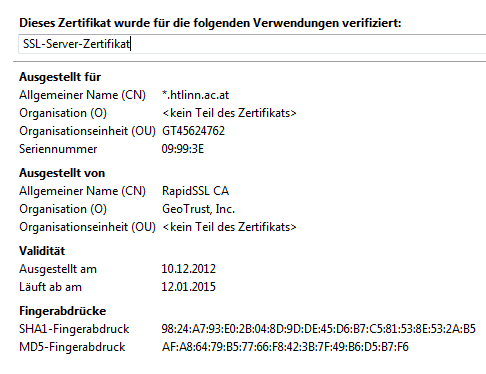
\includegraphics[keepaspectratio=true, width=12cm]{images/screenshots/certificate.png}
\caption{Allgemeine Zertifikatinforamtionen}
\label{fig:certificate}
\end{figure}
Die meisten Browser haben standardmäßig eine Liste von Zertifizierungsstellen eingetragen, welchen sie vertrauen. Diese Liste kann vom User jederzeit erweitert werden, jedoch sollte der User sich bezüglich der Seriosität der Zertifizierungsstelle wirklich sicher sein. 
\paragraph{Extended-Validation-Zertifikat}
Diese Zertifikate wurden entwickelt um eine höhere Sicherheit zu erhalten, als bei \enquote{normalen} Zertifikaten. Dies wird erreicht indem bei der Vergabe genauer kontrolliert wird. \\\\
Wenn bei einer Website ein erweitertes Zertifikat verwendet wird, wird in den meisten Browsern die Adressleiste komplett oder zumindest teilweise grün dargestellt.
\\
Bei der Vergabe dieser Zertifikate werden drei Kriterien besonders beachtet:
Die Identität und die Geschäftsadresse des Auftragstellers, ob der Antragsteller der ausschließliche Eigentümer der Domain ist oder ein exklusives Nutzungsrecht besitzt, ob die antragstellende Person überhaupt befugt ist und ob die rechtlichen Dokumente von zeichnungsberechtigten Personen unterschrieben wurden.

\subsubsection{Sicherheitsprobleme}
Eine Schwachstelle der oben genannten Arten des Schlüsseltausches ist jedoch ein Man-in-the-Middle. Dieser müsste vor Aufbau der Verbindung von Host1 und Host2 zwischen ihnen liegen. In Folge würde er jeweils mit Host1 und Host2 eine Verschlüsselung ausmachen. Wenn er nun die gesendeten Daten von Host1 an Host2 weiterleitet und umgekehrt, können die beiden Hosts dies nicht bemerken.\\
Jedoch benötigt der Man-in-the-Middle ebenso ein Zertifikat, in dem steht, dass er der Zielserver sei. Um dies zu bewerkstelligen, muss der Angreifer Zugang zu einer Zertifizierungsstelle besitzen und sich ein Zertifikat ausstellen lassen.
\subsection{Serverseitige Technologien}
\subsubsection{PHP (Handle)}
Die Abkürzung PHP steht für "PHP Hypertext Preprocessor". Es handelt sich hierbei um ein serverseitige Programmiersprache, die vor allem in der Webentwicklung zum Einsatz kommt. Die Syntax ist an Perl und C angelehnt.\\
Als PHP-Module wurden nur php5-mysql sowie php5-ldap verwendet.\\
PHP ist seit Version 5 vollständig Objekt-orientiert, wurde aber imperativ/funktional verwendet.\\
\\
Ein PHP Programm kann im Gegensatz zu anderen serverseitigen Programmiersprachen direkt in den HTML-Quelltext der Website eingebunden werden. Gekennzeichnet werden diese eingebetteten Programme mit den PHP-Tags (siehe Programm-Code \ref{lst:content_php_Tags}).\\
\begin{lstlisting}[style=custom, language=PHP,  caption={PHP-Tags},label={lst:content_php_Tags}]
<?php 
	/* Programm-Code */
?>
\end{lstlisting}
Befindet sich der PHP Code eingebettet in HTML-Quelltext, so ignoriert der Interpreter alles, das außerhalb der PHP-Tags steht.\\\\
Eines der großen Vorteile an PHP ist, dass es vollständig serverseitig verarbeitet wird, das heißt am Client wird keine Rechenleistung für das Ausführen des PHP-Codes benötigt.
\paragraph{Funktionsweise}
Der Client fragt am Webserver eine Datei mit der Endung .php an. Anschließend lädt der Webserver die Datei und übergibt diese dem PHP Interpreter. Dieser generiert in den meisten Fällen eine HTML Datei, welche anschließend dem Webserver übergeben wird. Dieser sendet die "fertige" Webseite an den Client. (siehe Abb. \ref{fig:content_php_PHP_Funktion}) Der PHP Interpreter ist nicht nur auf HTML Dateien begrenzt, es können auch andere Dateitypen, wie Bilder oder PDF Dateien generiert werden. Diese Funktionsweise hat das Problem, dass die Seite bei jedem neuen Aufruf erneut generiert werden muss, dies führt zu einer höheren Auslastung am Webserver. Um dieses Problem zu vermindern gibt es die Caches am Webserver, die häufig verwendete Programmteile zwischenspeichern, um sie bei erneutem Aufruf nicht erneut Interpretieren zu müssen.
\begin{figure}[H]
\centering
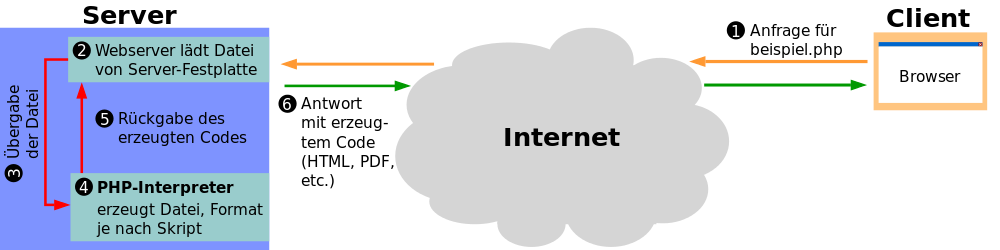
\includegraphics[keepaspectratio=true, width=14cm]{images/PHP_Funktionsweise.png}
\caption{PHP Funktionsweise}
\label{fig:content_php_PHP_Funktion}
\textbf{Quelle:} http://de.wikipedia.org/wiki/PHP
\end{figure}
\paragraph{PHP Sessions}
Mit PHP Sessions kann man einen Besucher einer Webseite über mehrere Aufrufe der Webseite hinweg genau identifizieren. Jedem Besucher auf der Webseite wird eine eindeutige Session-ID zugewiesen, diese wird in einem Cookie auf dem Server abgelegt. Eine PHP Seite, die die Session verwenden soll, muss als erstes des PHP-Dokuments diese Zeile stehen. (siehe Programm-Code \ref{lst:content_php_Session})
\begin{lstlisting}[style=custom, language=PHP, caption={Session},label={lst:content_php_Session}]
<?php
	session_start();
?>
\end{lstlisting}

Damit wird dem Webserver vermittelt, dass diese Seite mit einer Session arbeitet.\\
Die session-ID ist eine 128 Bit lange Zahl die zufällig generiert wird. Diese muss ab nun bei jeder Antwort vom Server an den Client mitgeliefert werden und auch umgedreht. Damit können personenbezogene Informationen einer bestimmten Session zugeordnet werden, wie ein Warenkorb bei Online-Shopping, Status von einer Anmeldung usw. Wir verwenden Sessions um den User über die Webseite hinweg identifizieren zu können. 
\paragraph{Kommunikation mit Server}
PHP hat auch eine Möglichkeit, um diverse Daten dem Server zu 
senden, diese können von der zu empfangenden Webseite verarbeitet werden.\\\\
Diese Funktion wird vor allem bei Formularen eingesetzt, um die User-Interaktion mit der Seite zu steuern. Es wird auch dazu verwendet um auf einer Seite zu navigieren oder ein Login bereitzustellen. Jedoch muss man in diesem Bereich im wesentlichen zwischen 2 Teile unterscheiden:
\begin{itemize}
    \item POST
    \item GET
\end{itemize}
\subparagraph{POST}
Bei POST werden die mitgegebenen Daten nicht an die URL angefügt, wie bei GET, aber dazu später, sondern werden im Body Teil der HTTP/S Anfrage an den Server. (siehe Programm-Code \ref{lst:content_php_HTTP_POST}) Dies hat den großen Vorteil, dass die mitgegebenen Daten praktisch eine unbegrenzte Größe haben können. Dadurch können auch lange Texte, Bilder, Dateien usw. an den Server gesendet werden. Ein weiterer Vorteil liegt darin, dass der User die eingegebenen Daten nicht sieht, d.h. gibt er ein Passwort ein so ist es für ihn nicht einsehbar. Dies schützt jedoch nicht vor Angreifer, die die HTTP Anfragen mitschneiden, deshalb verwendet man beim Senden von Passwörtern immer HTTPS.\\
Im Beispiel Programm-Code \ref{lst:content_php_POST} ist ein kleine Eingabe von einem Text möglich. Bei drücken des Buttons Speichern wird an den Server eine Anfrage gestellt, dass die gleiche Seite nochmals aufgerufen werden sollte, jedoch werden POST Variablen mitgegeben. Diese wertet die Seite mit dem PHP Teil aus und gibt den eingegebenen Text aus. Da dieser Text beliebig lang sein kann, muss POST verwendet werden. Warm siehe Punkt GET.
\begin{lstlisting}[style=custom, caption={Ausschnitt HTTP POST Request},label={lst:content_php_HTTP_POST}]
POST /login/index.php	//Angefragte Seite
HOST sis.htlinn.ac.at	//Host
	//Weitere Informationen
	//Weitere Informationen
	//Weitere Informationen
	//leere Zeile - Trennt Header von Body ab
user=20091234&password=passwort&send=1	//POST-Parameter
\end{lstlisting}
\begin{lstlisting}[style=custom, language=PHP, caption={Beispiel POST},label={lst:content_php_POST}]
<html>
<head>
</head>
<body>
<?php

if(!empty($_POST['text']))	//Wenn die Variable text nicht leer ist
	echo $_POST['text'];	//Soll der Text ausgegeben werden
else	//Wenn sie leer ist
	echo "nichts eingegeben";	//Soll eine Warnung ausgegeben werden
?>

<form method="post">	//method="post" --> Parameter werden mit POST mitgegeben
	<textarea name="text"></textarea>
	<button type="submit" name="save" value="Speichern">
</form>
</body>
</html>
\end{lstlisting}
\subparagraph{GET}
Bei GET werden die mitgegebenen Parameter direkt an die URL angehängt, um dies trennen zu können, wird die Parameterliste mit einem ? eingeleitet. Einzelne Parameter werden mit einem \& getrennt. Diese Methode ist die Standardmethode wenn man ein HTML-Form erstellt. Dies wird bei kleinen Daten verwendet. Der Vorteil liegt darin, dass der User die Seite neu laden kann und die Parameter werden übernommen. Auch kann der User die URL samt den Parametern als Lesezeichen abspeichern, um beispielsweise bei einer Webseite, die die Parameter zur Navigation auf der Seite verwendet, genau die gewünschte Seite zu erhalten. Eine Beispiel-URL sieht wie folgt aus: \textit{sis.htlinn.ac.at/index.php?text=hallo\&send=Speichern}. Dies wäre die URL, die bei absenden des Beispiel Programm-Codes \ref{lst:content_php_GET} entstehen würde. Sofern die Datei des Programm-Codes index.php heißt. Im Prinzip läuft die Auswertung der mitgelieferten Parametern gleich ab, wie bei POST Parametern.\\
Bei GET besteht die Grenze der Datenlänge darin, dass eine URL nur ca. 2000 lang sein darf, dies ist Browser und Server abhängig, aber 2000 Zeichen funktioniert bei allen Server-Client Kombinationen.
\begin{lstlisting}[style=custom, language=PHP,  caption={Beispiel GET},label={lst:content_php_GET}]
<html>
<head>
</head>
<body>
<?php

if(!empty($_GET['text']))	//Wenn die Variable text nicht leer ist
	echo $_GET['text'];	//Soll der Text ausgegeben werden
else	//Wenn sie leer ist
	echo "nichts eingegeben";	//Soll eine Warnung ausgegeben werden
?>

<form method="get">	//method="get" --> Parameter werden mit GET mitgegeben
	<input type="text" name="text"></textarea>
	<button type="submit" name="save" value="Speichern">
</form>
</body>
</html>
\end{lstlisting}
\subparagraph{URL-Encoding}
Die POST und GET Daten die an den Webserver gesendet werden, werden nicht exakt mit den Zeichen übertragen, die man zum Beispiel in ein Textfeld eingibt. Dies hat den Hintergrund, dass einige Zeichen reserviert sind und deshalb nicht in den GET oder POST Daten vorkommen dürfen. Um dies zu verhindern werden diese Zeichen mit anderen ausgetauscht. Dazu wird die Darstellung mit einem \% verwendet. Dabei wird das Zeichen mit der im entsprechendem Hexadezimalen ASCII Code und einem \% ausgetauscht.\\
Also wird die \# durch \%23 ausgetauscht, da die \# die Hexadezimale 23 im ASCII-Code darstellt.\\
Als reserviert gelten die Zeichen ! \# \$ \% \& ' ( ) * + , / : ; = ? @ [ ]. Jedes Leerzeichen wird durch ein + ausgetauscht, welches dann jedoch nicht URL-Codiert wird.
\paragraph{Probleme}
\subparagraph{Typisierung} 
Die Typisierung in PHP ist sehr flexible (dynamisch), so kann einer Variable, die zum Beispiel eine Zahl enthält, 
eine Zeichenkette, oder ein Array neu zugewiesen werden. \\
% typwechsel einer variable ist ja eher ein horror (IMHO)
Manche Standard-Funktionen in PHP haben numerische Rückgabewerte und geben den bool'schen Wert false zurück, 
wenn ein Fehler auftritt. Da alle Werte, die nicht 0 sind, laut Definition gleich dem bool'schen true sind, 
kann es zu Fehlinterpretation des Rückgabewertes kommen. Um solche Situationen so vermeiden, sollte statt auf Wertegleichheit (==) auf Äquivalenz (===), das bedeutet in diesem Zusammenhang Werte- und Typgleichheit (Bool != Integer, trotz dynamischer Typisierung), geprüft werden (Beispiel: siehe Programm-Code \ref{lst:content_php_false}).
\begin{lstlisting}[style=custom, language=PHP,  caption={false},label={lst:content_php_false}]
<?php 
	$string = "Hallo Welt";
	$position = strpos("H", $string); 
	// H liegt an Position 0
	
	// falsch:
	if ($position == false) {
		echo "Abfrage 1\n";
	}
	// richtig:
		if ($position === false) {
		echo "Abfrage 2\n";
	}
?>
\end{lstlisting}
\subparagraph{Serverseitige Realisierung}
Ein Problem und gleichzeitig auch ein Vorteil besteht darin, dass der Webserver die PHP-Datei compiliert 
und eine fertige HTML-Datei an den Client sendet. 
% Das muss er weil der Browser nur HTML versteht.
Der Vorteil liegt darin, dass keine Rechenleistung am Client nötig ist. 
% ausser zum Rendern. Der Vorteil ist, dass Daten angezeigt werden diese aber am Client nicht vorliegen
% z.B. Änderungszeitpunkt einer Datei oder Serveruhrzeit.
Jedoch bedeutet dies auch, dass ohne neue Anfrage zum Server und 
daraus resultierendes Neu Laden der ganzen Seite kann sich nichts am Seitenaufbau ändern. 
% daraus resultierendem Neuladen 
Soll sich z.B. bei Auswählen einer Check Box etwas am Aufbau der Seite ändern, 
so muss entweder die Seite neu geladen werden oder man greift auf andere Technologien zurück. 
(siehe \ref{sec:content_js_Javascript} oder \ref{sec:content_js_AJAX})

\subsubsection{MySQL (Handle)}
MySQL ist eines der bekanntesten und weit verbreitetsten relationalen Datenbankverwaltungssysteme auf der Welt. Ursprünglich wurde es von MySQL AB entwickelt, wurde jedoch von Sun Microsystems übernommen und ist jetzt in Händen von Oracle. Es ist als Open-Source Software oder als kommerzielle Enterprise Version verfügbar.\\
\paragraph{SQL\\}
Dieses Datenbankmanagementsystem verwendet als Sprache für den Zugriff auf die Datenbank SQL.\\
SQL steht für \textbf{Structured Query Language} und wurde dafür entwickelt, eine einheitliche und leicht lesbare Programmierschnittstelle zur Verfügung zu stellen, um Datenbanken zu bearbeiten.\\
SQL ist eine Datenbanksprache für relationale Datenbanken. Sie kann dazu verwendet werden, Datenbanken und Tabellen zu erstellen und bearbeiten, sowie um Datensätze zu bearbeiten - damit ist Löschen, Ändern oder Einfügen von Datensätzen in Tabellen gemeint. Außerdem können auch Datensätze abgefragt, gefiltert, sortiert und vieles mehr werden. Die Voraussetzung ist, dass das Datenbanksystem auf dieser Datenbanksprache basiert.\\
Hier die wichtigsten Befehle die verwendet wurden.\\
\subparagraph{Beispiele für Befehle}
\begin{itemize}
    \item SELECT
    	\begin{itemize}
	    	\item Mit \texttt{SELECT} können Datensätze aus Tabellen abgerufen werden. Zu diesem Befehl gibt es noch einige Zusätze, um zum Beispiel die Daten zu filtern, zu sortieren oder Tabellen miteinander zu verknüpfen.
	    	\begin{itemize}
		    	\item \texttt{SELECT * FROM classes;}\\
		    		Damit werden alle Datensätze aus der Tabelle classes ausgelesen.
		    	\item \texttt{SELECT short FROM teachers;}\\
			    	Damit wird nur die Spalte der Lehrerkürzel ausgelesen, jedoch von allen Datensätzen.
		    	\item \texttt{SELECT * FROM classes WHERE name LIKE '2 \%'}\\
		    		Damit werden alle Datensätze von Klassen ausgelesen, bei denen der Name mit 2 beginnt. So erhält man alle Klassen des 2. Jahrgangs.
		    	\item \texttt{SELECT * FROM substitudes ORDER BY time ASC}\\
		    		Damit werden alle Supplierungen in aufsteigender Reihenfolge(\texttt{ASC}) ausgelesen. Sollen die Supplierungen absteigend ausgelesen werden verwendet man statt \texttt{ASC DESC}.
		    	\item \texttt{SELECT teachers.name FROM classes LEFT JOIN teachers ON \\teachers.ID = classes.teacherFK}\\
		    		Mit dieser Abfrage können alle KV's der Klassen abgefragt werden. Da im Datenbankdesign auf Redundanzvermeidung geachtet wurde, wird in der classes Tabelle auf die teachers Tabelle verwiesen. Dort stehen die Namen der KV's. In der classes Tabelle steht nur die eindeutige ID des Lehrers.\\\\
		    		\textbf{\texttt{SELECT teachers.name FROM classes LEFT JOIN teachers ON \\teachers.ID = classes.teacherFK}}\\
		    			Gibt alle Einträge der Tabelle classes zurück, jedoch nur die Einträge von der teachers Tabelle, welche die \texttt{ON} Bedingung erfüllen.\\\\
		    		\textbf{\texttt{SELECT teachers.name FROM classes INNER JOIN teachers ON \\teachers.ID = classes.teacherFK}}\\
		    			Gibt nur diejenigen Datensätze zurück, welche die \texttt{ON} Bedingung erfüllen.\\\\
		    		\textbf{\texttt{SELECT teachers.name FROM classes RIGHT JOIN teachers ON \\teachers.ID = classes.teacherFK}}\\
		    			Gibt alle Einträge der Tabelle teachers zurück sowie nur die Einträge der Tabelle classes welche die ON Bedingung erfüllen.\\\\
		    		\textbf{\texttt{SELECT teachers.name FROM classes OUTER JOIN teachers ON \\teachers.ID = classes.teacherFK}}\\
		    			Gibt alle Einträge aus beiden Tabellen zurück. Die Einträge, welche die \texttt{ON} Bedingung erfüllen, werden zusammengefügt, und die anderen werden jeweils als einzelner Datensatz angezeigt.\\
		    	\item \texttt{SELECT name as Klassenname FROM classes}\\
		    		Mit as können die Spaltennamen der Tabelle in besser lesbare oder besser identifizierbare Spaltennamen umbenannt werden.
	    	\end{itemize}
    	\end{itemize}
    \item INSERT
	    \begin{itemize}
		   	\item Mit dem INSERT Befehl können neue Datensätze in eine Tabelle eingefügt werden.
		   	\begin{itemize}
			   	\item \texttt{INSERT INTO sections (name, short, teacherFK) VALUES \\('TestAbteilung', 'T', '2')}\\
			   		Damit wird eine neue Abteilung in der Tabelle sections erstellt. Dabei werden die angegebenen Spalten auf die in der Klammer stehenden Werte gesetzt. Hier muss die Spalte ID nicht angegeben werden, da sie auf \textit{auto increment} gesetzt ist.
		   	\end{itemize}
	    \end{itemize}
	\item UPDATE
		\begin{itemize}
			\item Mit dem UPDATE Befehl können Datensätze in einer Tabelle verändert werden.
			\begin{itemize}
				\item \texttt{UPDATE sections SET name = \\'TestAbteilung2' WHERE name = 'TestAbteilung'}\\
					Mit diesem UPDATE Befehl wird jeder Datensatz, der in der Spalte name \enquote{TestAbteilung} stehen hat, abgeändert. Dabei wird \enquote{TestAbteilung} in \enquote{TestAbteilung2} geändert.
				\item \texttt{UPDATE sections SET name = 'TestAbteilung123',short = 'T123' WHERE name = 'TestAbteilung2'}\\
					Dies Funktioniert im Prinzip gleich wie der Befehl zuvor. Mit dem Unterschied, dass dabei 2 Spalten geändert werden.
			\end{itemize}
		\end{itemize}
	\item DELETE
		\begin{itemize}
			\item Mit DELETE können einzelne Datensätze oder auch mehrere Datensätze auf einmal gelöscht werden.
			\begin{itemize}
				\item \texttt{DELETE FROM sections WHERE name = 'TestAbteilung123'}\\
					Damit werden alle Datensätze mit name = TestAbteilung123 gelöscht. Ohne dem WHERE Parameter werden alle Datensätze aus der Tabelle sections gelöscht.
			\end{itemize}
		\end{itemize}
	\item TRUNCATE
		\begin{itemize}
			\item Mit TRUNCATE können alle Datensätze aus einer Tabelle gelöscht werden. Im Unterschied zu DELETE wird hier auch der Index zurückgesetzt. Bei DELETE werden die neuen Datensätze fortlaufend weiter mit dem letzten Index nummeriert. Bei TRUNCATE beginnt die Nummerierung von vorne.
			\begin{itemize}
				\item \texttt{TRUNCATE FROM classes}\\
					Dabei wird die ganze Tabelle classes zurückgesetzt und damit auch alle Datensätze gelöscht. 
			\end{itemize} 
			
		\end{itemize}
\end{itemize}
\paragraph{Aufbau von MySQL}
Bei MySQL ist es im Normalfall so, dass die Datenbank/en auf einem MySQL Server liegen und die MySQL-Client/s Anfragen auf diesen Server senden.\\
Ein Server kann mehrere Datenbanken beinhalten. Eine solche Datenbank kann jeweils mehrere Tabellen beinhalten. Jede Tabelle hat mehrere Spalten.\\
Jede Spalte hat einen bestimmten Datentyp. Hier einige wichtige Datentypen, die benützt wurden:
\begin{itemize}
	\item TINYINT\\
	Wird für die Speicherung von BOOL Werten verwendet, da es den wenigsten Speicherplatz benötigt
	\item INT\\
	Wird für die Speicherung von Ganzzahlen verwendet.
	\item DATE\\
	Wird für die Speicherung von Datumsangaben verwendet.
	\item TEXT\\
	Wird für die Speicherung von Texten verwendet.
\end{itemize}
\paragraph{Verarbeitung von Anfragen}
Eine Anfrage, die an einen MySQL-Server gesendet wurde, wird grundsätzlich mit diesen Schritten abgearbeitet. Zuerst wird im Query-Cache nachgeschaut, ob ein gleicher Query schon einmal gestellt wurde und ob sich die Tabelle seither nicht mehr geändert hat. Ist es ein neuer Query, so wird der Query an den Parser gesendet und anschließend wird der Query optimiert, das Ergebnis wird zurückgeliefert.
\subparagraph{Query-Cache}
Wird ein Query an den MySQL-Server gesendet, wird zuerst im Query-Cache nachgeschaut, ob derselbe Query schon einmal gestellt wurde. Ist dies der Fall, so muss noch kontrolliert werden, ob sich die Daten in der Datenbank seither geändert haben. Hat sich nichts verändert, so sendet der MySQL-Server die gespeicherten Ergebnisse zurück. Dies hat den Vorteil, dass der MySQL-Server nicht wieder den Query ausführen muss und ist somit ressourcensparender. 
\subparagraph{Parsing}
Beim Parsing wird der gestellte Query in seine einzelnen Befehle zerlegt. Außerdem werden alle Informationen über den Query gesammelt. Zum Beispiel wird die Art(SELECT,DELETE,UPDATE,...) des Querys bestimmt. Ist das Parsing abgeschlossen, so ist ein so genannter Parse-Baum erstellt worden. Dieser wird anschließend optimiert.
\subparagraph{Optimierung}
In diesem Schritt wird der geparste Code optimiert. Dabei wird der Query analysiert, so werden die besten Abfragereihenfolgen ausgearbeitet. Es wird bestimmt, welche Tabellen wie und wann gejoined werden. Außerdem wird kontrolliert, ob alle Tabellen, die im Query vorkommen, auch wirklich benötigt werden.\\
Ist die optimale Abfragereihenfolge, gefunden wird der Query ausgeführt und das Ergebnis wird zurückgegeben.
\paragraph{Administration}
MySQL liefert standardmäßig einen Kommandozeilen-Client mit. Dieser kann in der Konsole mit \textit{mysql} aufgerufen werden. Damit können Datenbanken, Tabellen erstellt und bearbeitet werden, Datensätze können bearbeitet, verändert und gelöscht werden. Es können noch viele weitere Funktionen damit genutzt werden.\\
\subparagraph{Grafische Tools}
Es gibt noch zahlreiche grafische Tools, um MySQL Server zu administrieren. Eines der am weit verbreitetsten grafischen Tools ist phpMyAdmin. Dies ist ein Tool, das auf einen Webserver kopiert wird und es erlaubt, über ein Webinterface alle Einstellungen und Datenbankbefehle grafisch auszuführen. Dies erleichtert und vereinfacht das Erstellen, Bearbeiten und Verändern von Datenbanken und Tabellen. Damit können auch ungeübte Personen MySQL Datenbanken verwenden.
\paragraph{MySQL $ \Rightarrow $ PHP}
Um über PHP auf einen MySQL Server zugreifen zu können, benötigt man das PHP-Modul php5-mysql, welches einige Befehle zur Verfügung stellt, um mit einem MySQL-Server zu kommunizieren.\\
\subparagraph{Verbindung aufbauen}
Um mit einem MySQL-Server eine Verbindung aufzubauen müssen diese PHP Befehle verwendet werden(siehe Programm-Code \ref{lst:content_mysql_connect}).
\begin{lstlisting}[style=custom, language=PHP, caption={MySQL Connect},label={lst:content_mysql_connect}]
<?php 
	mysql_connect($host, $user, $passwd);
	mysql_select_db($db);
?>
\end{lstlisting}
In diesem Beispiel entspricht \texttt{\$host} der Adresse des MySQL-Server. \texttt{\$user} ist der Usernamen zum Anmelden auf dem MySQL-Server und \texttt{\$pass} ist das Passwort für die Anmeldung. Mit \texttt{\$db} wird die Datenbank angegeben, mit der gearbeitet werden soll. Die Funktion \texttt{mysql\_connect()} gibt im Fehlerfall \texttt{false} zurück und im Erfolgsfall einen Ressource Wert. \texttt{mysql\_select\_db()} gibt bei Erfolg \texttt{true} zurück, sonst \texttt{false}.
\subparagraph{Anfragen}
Um Anfragen an einen MySQL Server senden zu können, muss man diesen Syntax verwenden(siehe Programm-Code \ref{lst:content_mysql_query})
\begin{lstlisting}[style=custom, language=PHP, caption={MySQL Querys},label={lst:content_mysql_query}]
<?php 
	$sql="SELECT * FROM classes";
	mysql_query($sql);
?>
\end{lstlisting}
In der unter \ref{lst:content_mysql_query} gezeigtem Programmsequenz ist eine Anfrage an den MySQL Server gezeigt. Wichtig ist, dass zuvor die Zeilen vom \autoref{lst:content_mysql_connect} stehen, damit eine Anfrage an den Server gesendet werden kann. \texttt{mysql\_query} gibt bei Datenbankabfragen(\texttt{SELECT}, \texttt{SHOW}, \texttt{EXPLAIN}, ...) das Abfrageergebnis im Erfolgsfall zurück, bei Fehlerfall \texttt{false}. Wird ein anderer Datenbankbefehl(\texttt{INSERT}, \texttt{DELETE}, \texttt{UPDATE}, ...) ausgeführt, so gibt die Funktion bei Erfolg \texttt{true} und bei Misserfolg \texttt{false} zurück.\\
Das Ergebnis ist in Zeilen aufgebaut, d.h. will man jede Zeile abarbeiten, muss man jede Zeile zum Beispiel mit einer do-while-Schleife durchlaufen. Ein interner Positionszeiger verweist auf die momentane Stelle. Die Funktionen zum Abfragen dieser Zeilen stellt den Zeiger immer eine Stelle weiter.\\
Das Ergebnis bei einer Abfrage ist jedoch nicht in einem Format, mit dem man arbeiten kann, deshalb muss dieses Ergebnis noch an weitere Funktionen weitergegeben werden. Hier die von uns am häufigsten verwendeten Funktionen:
\begin{itemize}
	\item \texttt{mysql\_fetch\_array()}
	\begin{itemize}
		\item Mit dieser Funktion wird eine Zeile des Ergebnisses gelesen und in ein Array geschrieben. Zusätzlich wird der Positionszeiger eine Stelle weiter gestellt.\\
		Die Einträge des Arrays werden nummerisch indiziert und sind zusätzlich mit den Spaltennamen referenziert. Das heißt, die Ergebnisse sind in diesem Array doppelt vorhanden.
	\end{itemize}
	\item \texttt{mysql\_fetch\_object()}
		\begin{itemize}
			\item Mit dieser Funktion wird die aktuelle Zeile des Ergebnisses ausgelesen und als Objekt zurückgegeben. Wiederum wird der Positionszeiger eine Stelle weiter gestellt.
		\end{itemize}
	\item \texttt{mysql\_fetch\_row()}
		\begin{itemize}
			\item Diese Funktion gibt eine Zeile des Ergebnisses als Array zurück, das nummerische Indizes hat. Das heißt, hier sind aus dem Array die Spaltennamen nicht ersichtlich. Auch hier wird der Datenzeiger um eine Stelle weiter gestellt.
		\end{itemize}
\end{itemize}
Im Programm-Code \ref{lst:content_mysql_fetch_array} ist ein Ausschnitt einer Abarbeitung eines MySQL Results zu sehen. Hier wird zuerst ein Query an den Server gesendet und danach werden alle Ergebniszeilen durchlaufen und in ein Array gespeichert. Dazu wird \texttt{mysql\_fetch\_array()} verwendet.
\begin{lstlisting}[style=custom, language=PHP, caption={MySQL Query weiterverarbeiten},label={lst:content_mysql_fetch_array}]
<?php 
	$sql = "SELECT * FROM hours LIMIT 0,5"; //Mit LIMIT wird die Abfrage auf die ersten 5 Ergebnisse begrenzt
	$result = mysql_query($sql); //Ergebnis wird in der Variable $result gespeichert
	
	while($row = mysql_fetch_array($result)){	//Jede Ergebniszeile wird durchlaufen
		$ergebnis[] = $row;	//Hier wird die Zeile in einen Eintrag des Arrays geschrieben
	}
	
	print_r($ergebnis);	//Relationale Ausgabe des Arrays mit allen Zeilen
	
?>
\end{lstlisting}
Öffnet man den Quelltext der oberen Seite (Wiederum muss zuvor natürlich der Programm-Code \ref{lst:content_mysql_connect} in dem PHP-Code eingefügt werden, um überhaupt eine Verbindung mit dem MySQL-Server herstellen zu können.), so wird das Array \texttt{\$ergebnis} übersichtlich dargestellt. Das Ergebnis ist in der \autoref{fig:content_mysql_fetch_array} zu sehen.\\
Hier ist gut zu sehen, dass bei \texttt{mysql\_fetch\_array()} die Spalten nummerisch und laut Spaltenname indiziert werden. Dies kann durch den zweiten Parameter in der Funktion \texttt{mysql\_fetch\_array()} geändert werden. Außerdem ist hier zu sehen, dass jede Ergebniszeile einen eigenen Index (nummerisch Nummeriert) in dem Array \texttt{\$ergebnis} hat, daraus ergibt sich ein mehrdimensionales Array.\\
Auf die erste Zeile des Ergebnisses kann also mit \texttt{\$ergebnis[0]} zugegriffen werden. Das Ergebnis dieses Codes ergibt \autoref{fig:content_mysql_fetch_row}. Um dann auf die Start-Uhrzeit der Stunde von der ersten Zeile zugreifen zu können, kann man entweder den nummerischen Index oder die Spaltenbezeichnung verwenden. Also entweder \texttt{\$ergebnis[0][4]} oder \texttt{\$ergebnis[0]['startTime']}.\\ Das Ergebnis dieser Zeilen ist dasselbe, dieses ist in Abb. \ref{fig:content_mysql_fetch_column} zu sehen.\\
\begin{figure}[H]
\centering
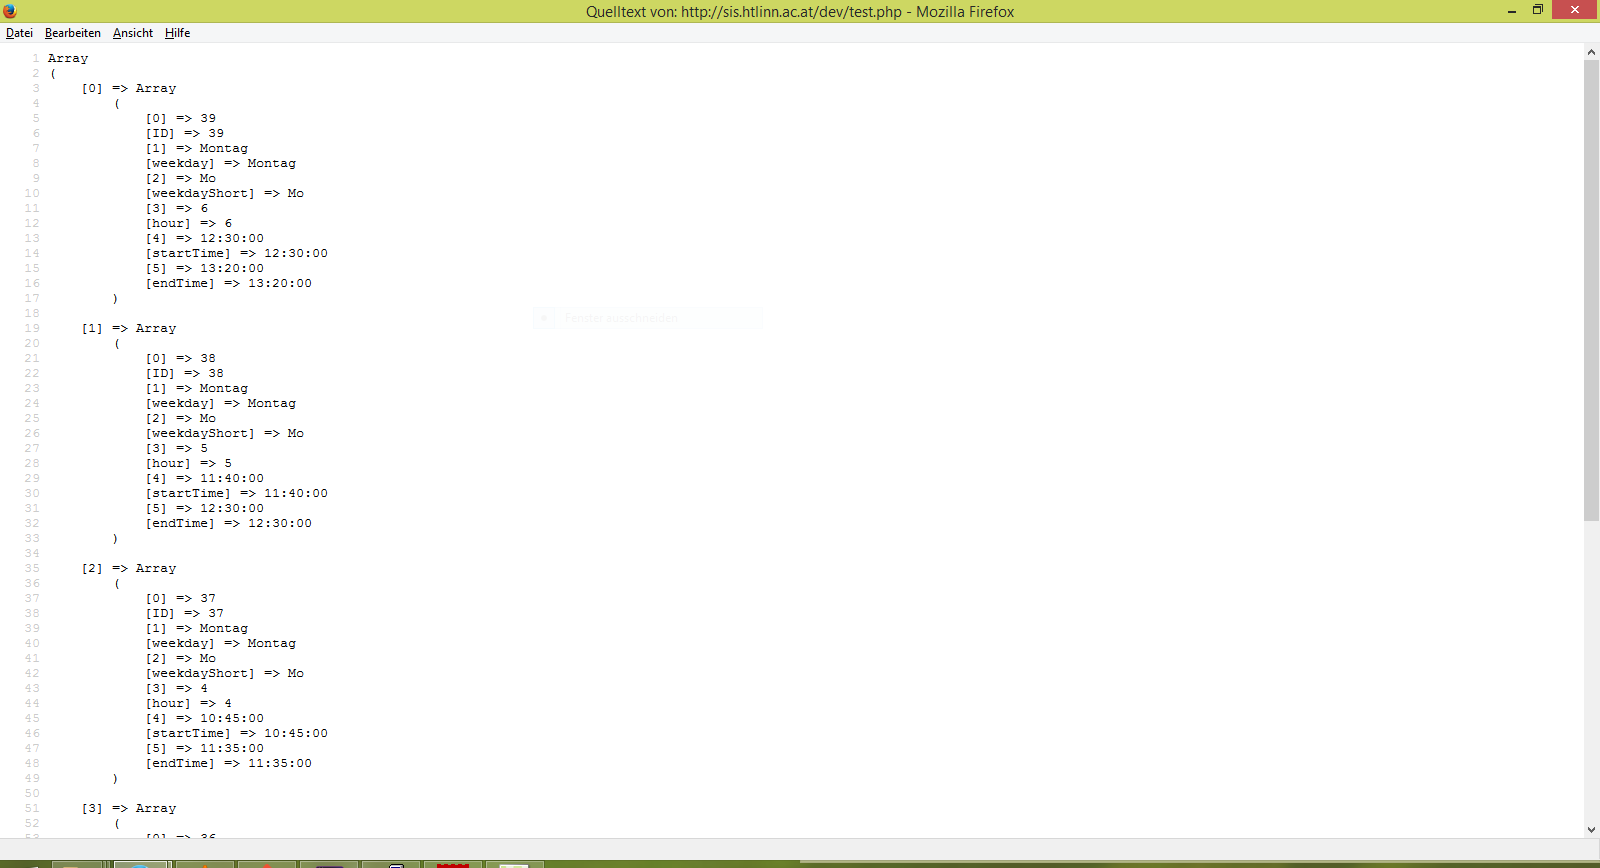
\includegraphics[keepaspectratio=true, width=14cm]{images/screenshots/content_mysql_fetch_array.png}
\caption{MySQL Fetch Array}
\label{fig:content_mysql_fetch_array}
\end{figure}
\begin{figure}[H]
\centering
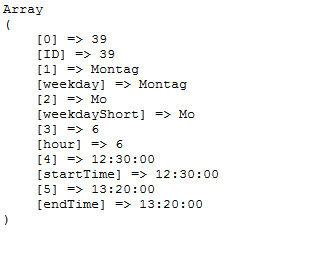
\includegraphics[keepaspectratio=true, width=8cm]{images/screenshots/content_mysql_fetch_row.png}
\caption{MySQL Zeile}
\label{fig:content_mysql_fetch_row}
\end{figure}
\begin{figure}[H]
\centering
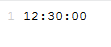
\includegraphics[keepaspectratio=true, width=3cm]{images/screenshots/content_mysql_fetch_column.png}
\caption{MySQL Spalte}
\label{fig:content_mysql_fetch_column}
\end{figure}
\subsubsection{Datenbank-Design (Buchberger)}

Bei relationellen Datenbanken, wie das für das Projekt verwendete MySQL, gelten grundsätzliche Richtlinien, um die Konsistenz der Daten zu gewährleisten:

\begin{description}[style=nextline]
	\item[Entitätsintegrität]
		Die Kennung eines Datensatzes (Primärschlüssel) muss auf jeden Fall eindeutig sein. Dies kann durch die MySQL-Eigenschaft \enquote{auto increment} erreicht werden.
	\item[Referenzielle Integrität]
		Verweise auf andere Tabellen (Fremdschlüssel) müssen auf Datensätze zeigen, die existieren. Alternativ kann NULL zugewiesen werden.\\
		\\
		\textit{Beispiel:} Ein Datensatz für eine Schulstunde hat einen Lehrer, auf den mit einem Fremdschlüssel verwiesen wird. Der Lehrer verlässt die Schule und sein Datensatz wird gelöscht.\\
		\\
		Die Stunde hat weiterhin den gleichen Fremdschlüssel, dessen Datensatz aber nicht mehr existiert.
	\item[Bereichsintegrität]
		Die Werte eines Datenfeldes müssen in einem definierten Bereich liegen.
\end{description}

Weitere wichtige Grundsätze sind:

\begin{description}[style=nextline]
	\item[Redundanzen sind zu vermeiden]
		Anders formuliert: Jede Information soll möglichst nur einmal in der Datenbank vorhanden sein.
		
		Redundanzen sorgen zwangsweise für Probleme, wenn Datensätze aktualisiert werden sollen.
		
		\textit{Beispiel:} Bei einem großen Unternehmen beliefert mehrere Kunden, welche im selben Ort wohnhaft sind. Ändert sich nun die Postleitzahl dieses Ortes, so müssen im Unternehmen alle Datensätze der Kunden aktualisiert werden.
		
		\textit{Lösung:} Auslagern des Ortes und der Postleitzahl in eine weitere Tabelle und via Fremdschlüssel verknüpfen.\\
		So muss bei Änderung der Postleitzahl nur an einer Stelle der Datenbank geändert werden.
		
		Es stellt sich allerdings die Frage, wie weit die Datenstruktur aufgefächert werden soll.
	\item[Gerechnet wird von der Datenbank]
		Das Programm, mit dem die Abfrage an die Datenbank gestellt wird, soll die Daten nicht mehr nachbearbeiten müssen.\\
		Gründe dafür sind, dass die Datenbank für die Verarbeitung von Daten optimiert ist, und dass es beim sequenziellen Abfragen von Tabellen zu Fällen kommen kann, in denen eine Tabelle bereits aktualisiert ist, die verknüpfte Tabelle allerdings nicht.
\end{description}

\subsubsection{LDAP (Buchberger)}

LDAP (Lightweight Directory Access Protocol) ist ein Protokoll für den Zugriff auf Verzeichnis-Datenbanken, wie Microsoft Active Directory, Apple Open Directory, openLDAP oder Novell eDirectory.\\
\\
Verzeichnis-Dienste werden dazu verwendet, um Informationen über Personen oder Rechner-Konfigurationen zu speichern und abzufragen.\\

\paragraph{LDAP-Datenstruktur}

Eine LDAP-Datenstruktur ist Baum-förmig (DIT - Directory Information Tree) aufgebaut.\\
Dies hat den Grund, dass man so geografische und/oder organisatorische Gegebenheiten besser in der Datenbank darstellen kann.
\\
Man unterscheidet zwischen Container-Objekten (enthalten ihrerseits weitere Objekte) und Blatt-Objekten (Sie stellen Enden des Baumes dar).\\
\\
LDAP ist objektorientiert aufgebaut, das heißt, es gibt Objekt-Klassen (wird durch das Schema difiniert), welche Eigenschaften der Objekte vorgeben. Ein LDAP-Objekt besitzt mindestens eine Klasse.\\
\\
Alle Objekte sind durch ihren DN (Distinguished Name) vollständig identifiziert. 
Der DN besteht aus dem Attribut, das das Objekt innerhalb des darüberliegenden Container-Objektes eindeutig macht, zusätzlich zum DN des Container-Objektes.\\
\\
\textit{Beispiel: }\\
uid=mueller,ou=beratung,ou=filliale1,c=at,o=firma\\
\\
Die uid=mueller identifiziert so ein Objekt (vermutlich ein Benutzer) in der ou=beratung. Diese ist wiederum einzigartig in der ou=filliale1, u.s.w.\\
\\
Das lässt sich nun so fortsetzen. Das obestere Container-Objekt wird als Root-Objekt bezeichnet. In den meisten Fällen wird dies mit dem Attribut o (für Organisation) gekennzeichnet.\\
\\
Die Eigenschaften der Objekt sind oft abgekürtzt.\\
\\
\textit{Häufige Abkürtzungen:}\\
\begin{description}[style=nextline]
	\item[o]
		organisationName (Organisation)
	\item[st]
		stateOrProvinceName (Staat/Provinz)
	\item[c]
		country (Land)
	\item[ou]
		organizational unit (Organisations Einheit)
	\item[cn]
		common name (Allgemeiner Name)
	\item[mail]
		e-mail-address (E-Mail-Adresse)
\end{description}

Die Objekt-Klassen definieren die Eigenschaften der Objekt.\\
\\
\textit{Beispiel: } Attribute der Objekt-Klasse inetOrgPerson (Definition des Standard-Schemas initOrgPerson von openLDAP in der Version 1.4.2.6)\\

\begin{description}[style=nextline]
	\item[erbt von]
		organizationalPerson
		\begin{description}[style=nextline]
			\item[erbt von]
				person
				\begin{description}[style=nextline]
					\item[erbt von]
						top	(abstrakte Klasse; keine Attribute)
					\item[!sn]
						sur name (Nachname)
					\item[!cn]
						common name (Allgemeiner Name)
					\item[userPassword]
						Benutzerpasswort
					\item[telephoneNumber]
						Telefon Nummer
					\item[seeAlso]
						Verweiß (als dn)
					\item[description]
						Beschreibung
				\end{description}
			\item[title]
				Titel
			\item[x121Address]
				wurde für das x.121-Protokoll verwendet
			\item[registeredAddress]
				Registrierungs Adresse
			\item[destinationIndicator]
				wurde für Telegram-Services verwendet
			\item[preferredDeliveryMethod]
				Bevorzugte Liefer Methode
			\item[telexNumber]
				wurde für Telex verwendet
			\item[teletexTerminalIdentifier]
				wurde für Teletex verwendet
			\item[telephoneNumber]
				Telefon Nummer
			\item[internationaliSDNNumber]
				ISDN Nummer
			\item[facsimileTelephoneNumber]
				Fax Nummer
			\item[street]
				Staßen Adresse
			\item[postOfficeBox]
				Postfach
			\item[postalCode]
				Postleitzahl
			\item[postalAddress]
				Post Adresse
			\item[physicalDeliveryOfficeName]
				Postbüro Name
			\item[ou]
				organisation unit (Organisations Einheit)
			\item[st]
				stateOrProvinceName (Staat/Provinz)
			\item[l]
				localityName (Ort/Ortschaft)
		\end{description}
	\item[audio]
		Audio
	\item[businessCategory]
		Geschäfts-Kategorie
	\item[carLicense]
		Fahrzeug-Lizenz
	\item[departmentNumber]
		Abteilung innerhalb eines Unternehmens
	\item[displayName]
		bevorzugter Anzeigename
	\item[employeeNumber]
		Angestellten Nummer
	\item[employeeType]
		Anstellungsart
	\item[givenName]
		Vorname(n)
	\item[homePhone]
		Heim-Telefon-Nummer
	\item[homePostalAddress]
		Heim-Andresse
	\item[initials]
		Initialen
	\item[jpegPhoto]
		JPEG Foto
	\item[labeledURI]
		Uniforme Resourcen ID mit optimaler Bezeichnung
	\item[mail]
		e-mail-address (E-Mail-Adresse)
	\item[manager]
		dn des Managers
	\item[mobile]
		mobile Telefon-Nummer
	\item[o]
		organisationName (Organisation)
	\item[pager]
		Telefon-Nummer des Pagers
	\item[photo]
		Foto
	\item[roomNumber]
		Raum Nummer
	\item[secretary]
		dn des Sekretärs
	\item[uid]
		Benutzer Kennung
	\item[userCertificate]
		Beuntzer Zertifikat		
	\item[x500uniqueIdentifier]
		ID für das X.500 Protokoll
	\item[preferredLanguage]
		bevorzugte Sprache
	\item[userSMIMECertificate]
		SignedData für S/MIME
	\item[userPKCS12]
		PKCS \#12 PFX PDU für den Austausch von persönlichen Identitäts-Informationen
\end{description}

\paragraph{LDAP-Suche}

Für die Suche in einer LDAP-Datenstruktur wird als erstes ein baseDN festgelegt, dieser entspricht dem Objekt, ab dem im Baum gesucht werden soll. Weiters wird der Scope festgelegt, hierbei gibt es 3 verschiedene Möglichkeiten:

\begin{description}[style=nextline]
	\item[base]
		Hierbei wird nur das Objekt mit dem baseDN durchsucht.
	\item[one]
		Eine Ebene unterhalb des baseDN wird gesucht.
	\item[sub]
		Alle darunter liegende Objekte sowie das, durch den baseDN referenzierte, werden durchsucht.
\end{description}
Die Suchkriterien werden in der Polnischen Notation (Präfixnotation) geschrieben und dürfen Wildcards enthalten.\\
\\
\textit{Beispiel:}\\
baseDN: ou=STUDENTS,o=HTLinn\\
scope: sub\\
(\&(l=5*H*)(mail=Andreas*)(cn=2009*))\\
\\
Diese Suchanfrage würde alle Objecte liefern, die
\begin{itemize}
	\item
		unterhalb von ou=STUDENTS,o=HTLinn liegen 
	\item	
		und die die Eigenschaften mail, l und cn enthalten
	\item	
		und bei denen der cn mit 2009 beginnt 
	\item	
		und deren E-Mail-Adresse mit Andreas beginnt 
	\item	
		und deren Ort-Attribut mit 5 beginnt und ein H enthält.
\end{itemize}
\subsection{Clientseitige 
Technologien}
\subsubsection{HTML (Weiland)}

HTML steht für "'Hypertext Markup Language"' und bezeichnet eine Auszeichnungssprache. HTML-Dateien werden hauptsächlich für Websites verwendet.


\paragraph{Aufbau}

Eine HTML-Datei ist grundsätzlich immer gleich aufgebaut. Sie besteht aus einem Header in dem unter anderem der Titel und die Meta-Daten bestimmt werden.
Im Body steht der Inhalt der Datei, welcher angezeigt werden soll. 
\begin{lstlisting}[style=custom, language=HTML, caption={HTML-Tags}]
<!DOCTYPE html>
<html> 
	<head>
		/* Datei-Kopf */
	</head>
	<body>
		/* Inhalt der Datei */
	</body>
</html>
\end{lstlisting}

\paragraph{HTML5}
HTML5 ist die aktuellste Version von HTML. Die Entwicklung begann am 29. April 2009 und soll im Jahr 2014 fertiggestellt werden.\\
Mit der Einführung von HTML5 kommen viele neue Elemente, wie zum Beispiel \enquote{details} und \enquote{summary}, zum HTML-Standard dazu. Dies Elemente sind zum Teil interaktiv, was im bisherigen Standard nicht möglich war. So wird zum Beispiel mit dem Element \enquote{details} eine Ausgabe erzeugt die ein-oder ausgeklappt werden kann ohne ein Script zu verwenden oder eine serverseitge Aktion zu erfordern.\\
Im Gegensatz zu früheren Versionen von HTML wird die Wiedergabe von Video- und Audiodateien unterstützt. Jedoch sind aktuell noch nicht alle Browser fähig, diese Funktionen zu verwenden.\\
Die unterstützten Formate sind für Videodateien 0gg Theora, MP4(H.264) und WebM(VP8) und für Audiodateien 0gg Vorbis, MP3 und Wav. \\
\begin{description}[style=nextline]
\item[in SIS verwendete Funktionen:]
\item[datalist] Liste von <option> Elementen, welche von anderen Elementen verwendet werden kann. Unter anderem verwendet um bei der Auswahl des angezeigten Stundenplans eine vorgefertigte Liste der Klassen und Lehrkräfte zu verwenden.
\item[video] Gibt ein Video aus. Bei uns wurde der Befehl (CODE EINFÜGEN) verwendet. Wobei die Option \enquote{autoplay} angibt ob das Video bei einem Seitenaufruf automatisch starten soll und die Option \enquote{loop} ob die Wiedergabe in einer Endlosschleife laufen  soll.
\item[source] Wird bei video und audio verwendet um verschiedene Quellen anzugeben. Somit verwendet jeder Browser die Quelldatei, welche er bevorzugt. Diese Option wurde bei der Wiedergabe des Videos verwendet, wobei als \enquote{src} der Speicherort des Videos und als \enquote{type} der Typ (z.B. video/mp4) der Datei verwendet werden muss. 
\end{description}
\subsubsection{Javascript (Klotz)}
\label{sec:content_js_Javascript}
JavaScript ist eine Skriptsprache welche für dynamische Erweiterungen im Webbrowser gedacht war. Es sollte helfen interaktive Websites, einfacher zu erstellen. Daher ist JavaScript auch nicht als alleinstehende Programmiersprache geeignet, und kommt fast immer in Kombination mit anderen Programmen oder Programmiersprachen zum Vorschein.\\
JavaScript wird hauptsächlich Clientseitig, das heißt im Webbrowser des Nutzers, genutzt um für den Nutzer Extras einzubauen. Dadurch wird auch der Server entlastet, da die Rechenleistung des Anwender-PCs genutzt wird und nicht die des Servers.\\
 Es gibt aber auch Serverseitiges-JavaScript(SSJS). Das kann dann, mit einem entsprechenden Interpreter (z.B.: Node.js), gleich wie andere Serverseitige Programmiersprachen verwendet werden.\\
JavaScript ist, wie die meisten Skriptsprachen, sehr einfach gehalten und Variablendeklarationen und ähnliches fallen weg(Variablentypen können auch während Laufzeit einfach verändert werden).\\
JavaScript ist eine Interpreter-Programmiersprache, das heißt, dass der Code erst im Webbrowser durch den integrierten Interpreter umgesetzt wird.\\
Obwohl JavaScript eine sehr einfache Programmiersprache ist, sind trotzdem alle wichtigen Strukturelement, wie Schleifen, If-Klauseln, etc. welche auch in anderen Programmiersprachen wie zum Beispiel C oder Java existieren, enthalten.\\
Weiters gibt es bei JavaScript die Möglichkeit Bibliotheken einzubinden. Dadurch kann man bereits vorgefertigte Funktionen einfach einbinden und anwenden. Ein Beispiel dafür ist JQuery.\\

\paragraph*{Anwendung}
Um JavaScript in einer Webseite zu nutzen gibt es zwei Möglichkeiten, entweder der Code wird direkt in das HTML-Dokument geschrieben(Variante1) oder man schreibt den JavaScript-Code in ein eigenes Dokument und bindet dieses dann ein(Variante2).\\
Variante 1\\
Wenn man den Code direkt in die HTML-Datei schreiben möchte, muss dieser Code dementsprechend markiert werden. Dazu verwendet man den Script-Tag (siehe Codebeispiel), dieser kann im Head oder im Body stehen, es ist jedoch üblich Funktionen in den Head zu schreiben.\\
\begin{lstlisting}
<html>
  <head>
    <script>
	//Here comes JS
    </script> 
  </head>
  
  <body>
  </body>
</html>
\end{lstlisting}


Variante 2\\
Im Gegensatz zur ersten Variante kommt in diesem Fall nur die Verlinkung zur JavaScript-Datei und nicht der ganze Code in das HTML-Dokument. Das eingebundene JavaScript-Dokument muss nicht auf dem gleichen Server oder Rechner gespeichert sein wie die Webseite, der Code kann sogar aus dem Internet geladen werden. Zum Einbinden einer JavaScript-Datei wird wieder ein Script-Tag verwendet, diesmal wird aber die URL der JavaScript-Datei als Attribut(„src = “) mitgegeben.\\
\begin{lstlisting}
<script src="js/jquery.js" type="text/javascript"></script>
\end{lstlisting}

\paragraph*{Funktionen}
In JavaScript kann man auch Funktionen schreiben, welche dann bei eintreten bestimmter Ereignisse ausgeführt werden. Der Code für eine JavaScript-Funktion sieht wie folgt aus:\\
\begin{lstlisting}
function functionname()
{
some code to be executed
}
\end{lstlisting}
Zwischen den geschwungenen Klammern wird der Code, der ausgeführt werden soll, geschrieben.\\
Um eine Funktion aufzurufen schreibt man den Funktionsnamen mit Klammern dahinter. Der Funktionsaufruf kann zwischen zwei Script-Tags geschrieben werden oder als bestimmtes Attribut (z.B. „onClick“) in manchen anderen Tags.\\
Bei einem Funktionsaufruf kann man der Funktion auch Werte mitgeben, dazu muss man in der Klammer hinter dem Funktionsnamen die Werte/Variablen eintragen. Die Mitgabe von Parametern muss natürlich in der Funktion vorgesehen werden, ansonsten werden die Werte einfach ignoriert.\\

\paragraph*{Variablen}
Bei JavaScript gibt es, wie auch bei anderen Programmiersprachen, Variablen. Diesen muss aber im Gegensatz zu Programmiersprachen wie C, Java oder ähnlichen, bei der Deklaration, kein eindeutiger Variablentyp zugewiesen werden. In JavaScript nur zwei Unterscheidungen bei den Variablentypen, nämlich in Zahlen und in Zeichen bzw. Zeichenketten. 
Um in JavaScript eine Variable zu deklarieren, schreibt man var und dann den Variablennamen. Um ihr dann noch einen Wert zuzuweisen muss man nur den Variablennamen und ein = Symbol schreiben, danach wird der gewünschte Wert hingeschrieben, falls es sich um eine Zeichenkette handelt muss man den Wert zwischen Anführungszeichen setzen:\\
\begin{lstlisting} 
var name = “Peter”;
var Anzahl;
Anzahl = 3;
name = "Hans";
\end{lstlisting}

Weiters muss man zwischen globalen und lokalen Variablen unterscheiden, während globale Variablen im gesamten Dokument definiert sind, sind lokale Variablen nur in der Funktion in der sie deklariert werden nutzbar. Um eine Variabel global zu definieren muss sie außerhalb jeglicher Funktionen definiert werden, wenn man eine Variabel aber innerhalb einer Funktion definiert handelt es sich um eine lokale Variable.\\

\paragraph*{Arrays}
In JavaSript gibt es auch Felder(Arrays). In diesen Feldern können sowohl Zahlen als auch Zeichen bzw. Zeichenketten gespeichert werden, es ist sogar möglich Zahlen und Zeichenketten in dasselbe Array zu speichern.\\
Einen Wert in einem Array zu speichern funktioniert gleich, wie einer Variable einen Wert zuzuweisen, aber bei einem Array muss man zusätzlich zum Arraynamen noch die angeben welchen Arrayeintrag man verändern möchte.\\
\begin{lstlisting}
var cars = new Array();
cars[0] = "Audi";
cars[1] = "BMW";
cars[2] = "Mercedes";
\end{lstlisting}

\paragraph*{JSON}
JSON (JavaScript Object Notation) ist ein Datenaustauschformat welches so gestaltet ist, dass Menschen es leicht lesen können und der Computer es einfach parsen kann. Es basiert auf JavaScript.\\
JSON wird sehr häufig in Verbindung mit JavaScript verwendet, kann aber auch mit anderen Programmiersprachen verwendet werden.\\
Beispiel für ein JSON-Objekt:\\
\begin{lstlisting}
{
  "Gerät": "Auto",
  "Marke": "Audi",
  "Farbe": "rot",
  "Seriennummer": 02345032,
}
\end{lstlisting}

Die Daten werden in Form von Daten-Wert Paaren gespeichert. Aus diesem Objekt kann man nur relativ einfach Daten auslesen. Der JavaScript-Code um die Marke auszulesen würde zum Beispiel wie folgt aussehen:
var Marke = object.Marke;


\subsection{Mobil App (Klotz)}

\subsubsection{PhoneGap}
PhoneGap ist ein Framework, von Adobe Systems, um mobile Apps zu erstellen. Diese Apps sind jedoch weder Web-Apps noch native Apps. Hierbei handelt es sich um Hybrid-Apps. Das heißt die App verwendet nicht die nativen Userinterface Frameworks um das Layout zu gestalten, sondern Web-Technologien, aber die App arbeitet trotzdem vollkommen lokal auf dem Gerät.\\
Das funktioniert indem die App praktisch im Webbrowser des eigenen Gerätes ausgeführt wird, aber alle browsertypischen Eigenschaften, wie zum Beispiel der Rahmen, die URL-Leiste oder die Einstellungen deaktiviert oder ausgeblendet werden.\\
Im Gegensatz zu herkömmlichen Web-Applikationen, kann man mit PhoneGap-Apps auch auf Funktionen wie zum Beispiel den Beschleunigungssensor oder die Kamera zu nutzen. Das wird durch die PhoneGap API ermöglicht. Dabei handelt es sich um Java-Dateien die bei der Installation der App heruntergeladen werden. Mit JavaScript kann man dann über diese Java-Dateien auf die Geräteinternen Sensoren zugreifen. Es handelt sich hierbei also um einen Kompromiss aus Web-Entwicklung und nativer App-Entwicklung.\\
Um PhoneGap zu nutzen muss man sich für alle Systeme, auf denen die App nach der Entwicklung betrieben werden soll, ein SDK installieren, zum Beispiel für Android Eclipse, für iOS XCode oder für WindowsPhone das Microsoft SDK. In dieses SDK muss nun PhoneGap als Plugin geladen werden und mit diesem Plugin kann man die App auch mit Webtechnologien (HTML, CSS, JS) anstatt gerätespezifischer Programmiersprachen (Java, ObjectiveC, VisualC) entwickeln.\\
Unterstützte mobile Betriebssysteme bis Version(2.9):\\
					Android\\
					IOS\\
					Windows Phone 7 \& 8\\
					Blackberry\\
					WebOS(HP)\\
					Tizen\\
					Symbian\\
					Bada\\
Ab PhoneGap-Version 3.0 werden nur noch Android, iOS und Windows Phone unterstützt.\\

PhoneGap basiert auf dem Open-Source-Projekt Apache Cordova. Daher darf PhoneGap auch vollkommen kostenlos genutzt werden.\\
\paragraph{PhoneGapBuild\\}
Für dieses Projekt wurde PhoneGapBuild verwendet.\\
Bei PhoneGapBuild handelt es sich um eine Online-Variante von PhoneGap. Diese wird von AdobeSystems kostenlos zur Verfügung gestellt. Der Vorteil dieser Variante ist, dass nicht für jedes Betriebssystem, für das die App entwickelt werden soll, eine eigene SDK installiert werden muss, da die Applikation direkt online kompiliert wird.\\
Den Code kann man entweder in Form einzelner HTML-, CSS-, und JS-Dateien verpackt als ZIP-Datei hochladen, oder ein GitHub Projekt angeben in dem sich der Code befindet.\\
Nach dem Hochladen des Codes wird die App online sofort kompiliert und die Installationsdateien(APK, XPA, etc.) werden als Download zur Verfügung gestellt.\\

Für die App-Entwicklung mit PhoneGapBuild benötigt man ausschließlich einen Editor und einen Webbrowser, da es sich ja eigentlich um Webentwicklung handelt. Die App besteht nur aus einer(oder mehreren) Webseite(n), welche mit CSS gestaltet wird. Um die Applikation interaktiv zu gestalten, kann man mit JavaScript-Skripts arbeiten und diese auch integrieren. Im Gegensatz zur Webentwicklung gibt es bei der App zusätzlich noch eine Datei mit dem Namen config.xml. In dieser Datei stehen alle Informationen, wie zum Beispiel die Versionsnummer oder der Name, zu der App und anhand dieser Datei können Berechtigungen für den Zugriff auf das Gerät vergeben werden.\\

\subsubsection{iOS}
iOS ist das mobile Betriebssystem von Apple, es wird nur auf IPhones und IPads betrieben. Das Betriebssystem basiert auf dem MacOSX-Kern und somit auch auf einem Unix-Kern.\\
Mit iOS vermarktet Apple den größten Konkurrenten von Android, obwohl das System nur auf den eigenen Geräten installiert wird, ist iOS das am 2. häufigsten genutzte mobile Betriebssystem mit ca. 13\% Marktanteil.\\
\paragraph*{Appstore\\}
IPhone- bzw. IPad-User können Applikationen für ihre Geräte im Appstore herunterladen.\\ 
Eine Besonderheit an iOS ist, dass Apps ausschließlich aus dem Appstore geladen werden können. Das soll mehr Sicherheit und Kontrolle bieten.\\
Um eine Applikation in den Appstore zu laden muss man Developer sein, wofür man wieder um jährlich 99\$ zahlen muss. Für das Veröffentlichen selbst muss man aber keine weiteren Gebühren bezahlen, aber Appel bekommt ca. 30\% der Einnahmen wenn die App kostenpflichtig ist.\\
\paragraph*{PhoneGap mit iOS\\}
Im Laufe des Projekts wurde eine Möglichkeit gefunden den Appstore zu umgehen. Wenn man eine iOS-Applikation mit dem Dienst „PhoneGap Build“ von Adobe erstellt, benötigt man zwar die geeigneten Zertifikate von Apple, das heißt man muss trotzdem als Developer angemeldet sein und jährlich 99\$ bezahlen, aber wenn man nun mit dem IPhone oder IPad dem Downloadlink folgt kommt anstatt des üblichen Downloads die Frage ob man die App installieren will.
Wenn es sich bei den ausgestellten Zertifikaten um Distribution-Zertifikate handelt, ist es so möglich die App auf allen iOS-Geräten zu installieren ohne sie in den Appstore zu stellen. Um diese Funktion zu ermöglichen wurde wahrscheinlich ein Abkommen zwischen Apple und Adobe geschlossen.\\

\subsubsection{Android}
Android ist ein Betriebssystem für Smartphones, welches von Google entwickelt wird. Es basiert auf einem Linux-Kernel.\\
Bei Android handelt es sich um das am weitesten verbreitete mobile Betriebssystem, es hat einen Marktanteil von ca. 80\%. Es wird als freie Software gehandelt und wird als Open-Source entwickelt.\\
\\
\paragraph*{Architektur\\}
Android baut wie bereits erwähnt auf einem Linux-Kernel auf.  Dieser stellt eine Schnittstelle zwischen der Hardware und der höher gelegenen Software dar.\\
In der nächsthöheren Systemschicht sind Android-Klassenbibliotheken, durch welche man die Funktionen des Kernels nutzen kann. Zusätzlich befindet sich auf dieser Ebene eine Dalvik-Virtual-Machine, dabei handelt es sich um eine virtuelle Maschine in der die Applikationen ausgeführt werden.\\
Diese virtuelle Maschine wurde von Google entwickelt und ähnelt in ihrer Funktionalität sehr der Java-VM. Die virtuellen Maschinen führen den Bytecode der Applikationen aus, aber die Dalvik Maschine arbeitet als Registermaschine, weshalb normaler Java-Bytecode auf Android nicht funktioniert.\\
Android startet für jede gestartete Applikation eine eigene virtuelle Maschine, dadurch kann keine App direkt auf das System zugreifen sondern nur über die virtuelle Maschine und des weiteren können sich die Apps nicht gegenseitig stören oder beeinflussen, dadurch dass sie in verschiedenen virtuellen Maschinen betrieben werden.\\
\\
\paragraph*{Store\\}
Im Google Play Store sind viele Apps für Android verfügbar. Dieser Store ist komplett kostenlos nutzbar, jedoch gibt es kostenpflichtige Applikationen. Um Apps aus dem Play-Store zu installieren muss man aber einen Google-Account besitzen welcher auch komplett kostenlos ist.\\
Bei Android kann man den Store relativ einfach umgehen, denn bei Android kann man alle APK-Files(Android-Installationsdateien) einfach ausführen. Dazu muss man nur in den Einstellungen im Menü Anwendungen, den Punkt Unbekannte Quellen aktivieren. Damit erlaubt man das Installieren von Apps die nicht aus dem Play-Store heruntergeladen werden.\\
Ist das erledigt muss man nur noch das gewünschte APK-File auf dem Smartphone speichern (downloaden oder über USB auf dem Smartphone speichern) und dieses dann öffnen. Dann wird die Applikation automatisch installiert und ist danach wie jede andere Applikation auf dem Gerät installiert.\\
 Um Apps in den Play-Store hochzuladen muss man als Entwickler registriert sein. Eine Registrierung als Entwickler kostet einmalig(Registrierungsgebühren) 25\$. Nach dieser Registrierung kann man kostenlos so viele Apps hochladen wie man will, bei kostenpflichtigen Apps verlangt Google jedoch ca 30\% der Einnahmen.\\



\subsubsection{Windows Phone}

\subsubsection{Sonstiges}


\section{Lösungswege}

\subsection{PHP}
% Warum PHP? Welche Alternativen gäbe es?
\subsection{MySQL}
% Warum MySQL? Welche Alternativen gäbe es?
\subsection{Datenbankdesign}
Bei Design der Datenbank stellten sich einige grundlegenden Fragen:

\begin{itemize}
	\item Wie werden die Schulstunden gespeichert?
	\item Wie werden die Supplierungen gespeichert?
\end{itemize}

\subsubsection{Gewählte Lösung}
Die Gruppe entschied sich für folgende Lösung:\\
\\
Es gibt Tabellen für:\\
\begin{itemize}
	\item Abteilungen
	\item Klassen
	\item Fächer
	\item Lehrer
	\item Uhrzeiten
\end{itemize}
\vspace{0.03cm}
\begin{itemize}
	\item Die Basis-Stunden
	\item Die Stunden
\end{itemize}
\vspace{0.03cm}
\begin{itemize}
	\item fehlende Lehrer
	\item fehlende Klassen
\end{itemize}
\vspace{0.03cm}
\begin{itemize}
	\item Die Supplierung
\end{itemize}
Die Basis-Stunde verknüpft die Klasse der Stunde mit der Uhrzeit. Die Stunde verknüpft die Basis-Stunde mit dem Lehrer, dem Fach und dem Raum.\\
\\
Die Basis-Stunde wird benötigt, damit die Information, welche Klasse wann Unterricht hat, nicht mehrfach gespeichert werden muss.\\
\\
Die Tabellen für die fehlenden Lehrer und die fehlenden Klassen haben Spalten für eine Start- und End-Zeit.\\
\\
Die Supplierungs-Tabelle hat Felder für die Stunde, den Supplierlehrer, den neuen Klassenraum, die neue Start- und Endstunde, sowie Flags zum Ausblenden der Stunde auf dem angepassten Stundenplan.\\
Es ist möglich, mehrere Supplierungen für die gleiche Stunde einzutragen. Dieses Verhalten ist für manche Ausnahmefälle notwenig (siehe Beispiel).\\
\\
\begin{figure}[H]
\centering
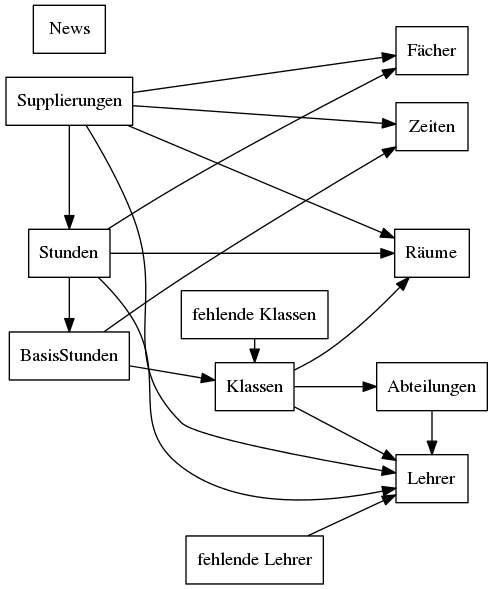
\includegraphics[keepaspectratio=true, width=10cm]{images/dbSubstitudes.png}
\caption{Supplierungs-Datenbank}
\end{figure}
Für das folgende Beispiel wird angenommen, dass eine Schulstunde 60 Minuten entspricht.\\
\\
\textit{Beispiel:} Klasse K hat am Montag um 8:00 eine Doppelstunde des Faches F mit Lehrer L in Raum R. Da der Lehrer zu spät kommen wird (ist bereits im vorhinein bekannt), soll nun die erste Stunde auf 16:00 in Raum P verschoben werden, die zweite Stunde soll aber bleiben.\\
\\
\textit{Lösung:} Die Doppel-Stunde wird 2 mal suppliert. Einmal mit dem selben Lehrer im selben Raum mit Start-Stunde um 9:00 und End-Stunde um 10:00. Und das zweitemal mit dem selben Lehrer im Raum P mit Start-Stunde um 16:00 und End-Stunde um 17:00.

\subsubsection{Alternative Lösungen}

Eine alternative Lösung, die angedacht wurde, ist folgende:\\
\\
Ansatt zwei Tabellen für die Basis-Stunde und die Stunde gibt es nur eine Stunden-Tabelle.
Diese verknüpft die Klasse mit der Uhrzeit, der Länge der Stunde, einem kombinierten Lehrer-Feld, einem kombinierten Fächer-Feld, einem kombinierten Raum-Feld.\\
\\
Die kombinierten Felden sollten den ersten Wert enthalten. Für jeden weiteren Wert wird der aktuelle Feld-Wert verodert mit dem nächsten Wert, welcher zuvor um ($x \cdot $(Anzahl der bisherigen Einträge)) Bits nach links verschoben wurde.\\
Hierbei wurde \textit{x} noch nicht bestimmt, es müsste so gewählt werden, dass der Eintrag mit der höchsten ID nicht in den dahinterliegenden Einträg überläuft (Für die Lehrer wäre $2^{8}$ (=256) ideal, da es knapp unter 200 Lehrer an der HTL gibt).\\
\\
Diese Lösungsmöglichkeit wurde allerdings verworfen, da es einiges an Aufwand ist, immer die richtigen Lehrer herauszulesen und da das Holen der Lehrer-Daten (Name, etc) nicht mehr im selben Query ausgeführt werden kann, als das Holen der Stundendaten, was bei mehr als 1 Zugriffspunkt zu Problemen mit der Daten-Konsistenz führen kann.
\subsection{HTTPS}

\subsubsection{Gewählte Lösung}

\subsubsection{Alternative Lösungen}
\subsection{Mobile App}

\subsubsection{Gewählte Lösung}

\paragraph*{Hybrid-App\\}

Die App wird als Hybrid-App realisiert, dabei handelt es sich um eine Applikation welche zwar mit Webtechnologien erstellt wird aber lokal auf dem Gerät betrieben wird.
Die mobile App wird aus Webseiten mit HTML, JavaScript und CSS aufgebaut. Diese Dateien werden dann mit Hilfe des Frameworks PhoneGap zu einer App für Android, WindowsPhone und iOS kompiliert. Zur Kommunikation mit dem Server sind noch einige PHP-Dateien auf dem Server gespeichert.


\subsubsection{Alternative Lösung}
\paragraph*{Native App\\}

Es könnte auch eine native App erstellt werden dann müsste aber für jedes der drei Betriebssysteme eine eigene App erstellt werden.\\
\\
Android:\\
Native Android-Apps werden grundsätzlich in Java programmiert. Um solche Applikationen zu erstellen wird aber gewisse Software benötigt.\\
Es muss eine Entwicklungsumgebung (IDE), zum Beispiel Eclipse, auf dem Rechner installiert werden und nachträglich müssen noch die Android Development Tools (ADT) installiert werden. Alternativ gibt es noch die Möglichkeit Android Studio von Google zu installieren, dabei handelt es sich um eine vollständige Android-Entwicklungsumgebung, mit einigen Extras wie zum Beispiel einem Layout-Editor.\\
\\
WindowsPhone:\\
WindowsPhone-Apps werden in C\# programmiert.\\
Zum erstellen einer WindowsPhone-App muss zuerst VisualStudio installiert werden. Damit können dann Apps für WindowsPhone entwickelt werden. In VisualStudio ist sogar ein Simulator integriert mit welchem es möglich ist die Apps zu testen bevor man sie auf ein Smartphone lädt.\\
\\
iOS:\\
Für die Entwicklung einer iOS-Apps benötigt man als erstes einen Mac(Apple-Computer), da es die Entwicklungssoftware für iOS-Apps(XCode) nur für Mac gibt.\\
Um eine iOS Applikation zu erstellen muss man zuerst die Entwicklungssoftware, XCode, herunterladen und installieren. Mit Hilfe dieser Software kann man nun erste Apps erstellen. Die grafische Oberfläche der App kann man noch sehr einfach durch Drag and Drop Funktionen erstellen. Um den Schaltflächen jedoch Funktionen zuzuweisen muss man auch wieder programmieren. Bei der verwendeten Programmiersprache handelt es sich um Objective-C, eine objektorientierte Programmiersprache mit Ähnlichkeiten zu C++ und C\#.
Die programmierten Applikationen kann man dann im integrierten Simulator testen.
Um die Applikationen auf echten Geräten zu testen benötigt man bereits eine Entwicklerlizenz, diese kostet 99\$ pro Jahr(Preis von https://developer.apple.com/programs/ios).\\
\\
Native Applikationen sind zwar wesentlich schneller als hybrid Apps, aber diese Lösung wurde nicht gewählt, da es viel zu aufwendig ist für jedes Betriebssystem eine eigene Entwicklungsumgebung zu installieren und die App drei mal in den jeweiligen Programmiersprachen zu programmieren und zu erstellen. Und da keiner der an der Diplomarbeit beteiligten Schüler ein PC von Apple besitzt wäre es uns nicht möglich gewesen eine iOS-App auf diesen Weg zu erstellen.\\

\paragraph*{Web-App\\}

Eine weitere Alternative ist die Entwicklung einer Webapp.\\
Bei einer Webapp handelt es sich prinzipiell um eine Webseite, welche für Smartphones optimiert wurde, beim Öffnen der Applikation wird einfach die gewünschte Webseite geladen.\\
Die Entwicklung einer Webapp würde sich kaum von der Entwicklung einer hybrid App unterscheiden, aber bei der Webapp hat man den Vorteil, dass auch PHP-Seiten verwendet werden können. Dadurch ist die Übertragung der Daten und die Authentifizierung wesentlich einfacher.\\
Eine Webapp hat aber den Nachteil, dass sie langsamer ist als eine Applikation welche lokal auf dem Gerät installiert ist und ein weiterer Nachteil für den Nutzer ist, dass bei dieser Lösung ein wesentlich größerer Bedarf an Internetdatenvolumen anfällt.\\

% warum phonegap, was wären die alternativen gewesen? vor-, nachteile?
\subsection{Prinzip des Monitor-Systems}

Als Thin-Client für die Monitore werden Raspberry Pis verwendet.\\
Die Kommunikation zum Server und die Art des Anzeigens der abgerufenen Informationen wird mithilfe eines Webbrowsers gelöst. Es wurde der Webbrowser Chromium ausgewählt, da dieser die neuesten HTML5 Standards implementiert hat und auf den Raspberry Pis laufen kann.

\subsubsection{Laden der Daten}

Für das Laden der Daten vom Webserver wird Javascript in Verbindung mit AJAX verwendet.\\
Dies hat gegenüber dem Neuladen der Seiten den Vorteil, dass, im Falle dessen, dass der Webserver kurzzeitig nicht erreichbar ist, das System trotzdem ohne Probleme weiter laufen kann - sieht man davon ab, dass mit der zeit, die angezeigten Daten veralten.\\
Der einzige Zeitpunkt, an dem der Server auf alle Fälle erreichbar sein muss, ist der Start der Raspberry Pis, da hier die Website vom Server geladen werden wird. Auch diese Bedingung hätte entfernt werden können, indem man die Seite lokal abgelegt hätte. Dies hat allerdings den Nachteil, dass die Seite über ein weiteres Script hätte immer auf dem aktuellen Stand gebracht werden.

\subsection{Authentifizierung der Monitore}

Es stellt sich die Frage, die die Monitore am Server registriert werden. Da alle Monitore über das Webinterface zentral administriert werden können, ist es äußerst kontraproduktiv, wenn eventuell Schüler - oder gar Außenstehende - die Datenbank-Tabelle für die registrierten Monitore fluten können.\\
\\
Es wurde von den Betreuern vorgegeben, dass für sämtliche Verbindungen zum Server HTTPS verwendet werden sollte (siehe Lösungswege/HTTPS). Dies führt bei der Registrierung der Monitore zu Problemen (siehe folgendes).

\subsubsection{Gewählte Lösung}

Da zu anfangs nicht klar war, welches IP-Netz das W-LAN der Monitore bekommen sollte, konnte keine IP-Filterung verwendet werden.\\
\\
Das Problem wurde gelöst, indem in der Datenbank für die Monitore eine Spalte für die IP-Adresse vorgesehen wurde. Die Idee bestand darin, dass jede IP-Adresse nur maximal einen Monitor registrieren darf (Vgl. \autoref{sec:content_solutions_monitors_alt_reg}).\\
\\
Aufgrund dessen, dass für die verschlüsselte Verbindung die Packete nach außen geNATet werden und wieder durch die Firewall zurück kommen, haben alle Monitore die öffentliche IP-Adresse der Schule.\\
Um dieses Problem zu umgehen wurde mit Betreuer Lassnig vereinbart, dass die Verbindung der Monitore unverschlüsselt sein darf, da keine sicherheitsrelavanten Daten übertragen werden, und da das W-LAN selbst schon verschlüsselt.\\
Als Ziel-Adresse wird also anstatt https://sis.htlinn.ac.at http://sis.clients.htlinn.ac.at eingetragen.


\subsubsection{Alternative Lösungen}

\paragraph{Registrierung}
\label{sec:content_solutions_monitors_alt_reg}

Die Registrierung der Monitor hätte manuell erfolgen können. Hier würden mehrere Möglichkeiten in Frage kommen:

\begin{description}[style=nextline]
	\item[Registrierung nur vom Administrator-Interface aus]
		Dies hat den Nachteil, dass es zu frustrierenden Situationen kommen kann, wenn der tatsächliche Name des Monitors (eingestellt im Raspberry Pi) mit dem in der Datenbank nicht identisch ist.\\
	\item[Registrierung mittels Passwort]
		Ein Nachteil dieser Variante ist, dass das Passwort direkt an den Raspberry Pis eingegeben werden muss. Was den administrativen Aufwand vergrößert.
		Weiters muss dieses Passwort für Konfiguration mehr oder weniger öffentlich zugänglich sein muss, was den Zusatzaufwand nichtig macht.
	\item[Registrierung mittels Cookie-Hash]
		Diese Variante hat ähnliche Nachteile, wie die Registrierung mittels Passwort.
\end{description}

\paragraph{Verschlüsslung}

Als Alternative zur fehlenden Verschlüsslung hätte ein, von der HTL ausgestelltes SSL-Zertifikat für die Wild-Card-Domain *.clients.htlinn.ac.at ausgestellt werden können, den Raspberry Pis hätte man dann müssen das HTL-Root-Zertifikat importieren müssen. Dies ist allerdings mit recht viel administrativen Aufwand verbunden, daher wurde diese Idee verworfen.\\
Als eine weitere Variante hätte man den Raspberry Pis den Server, auf dem die Website abgelegt wurde, als SSL-Ausnahme eintragen können. 
\subsection{Benutzermanagement}
In der Schule sind im Wesentlichen 4 Berechtigungsstufen vorhanden.
\begin{itemize}
	\item Schüler
	\item Lehrer
	\item Abteilungs-Vorstände
	\item Administratoren
\end{itemize}
Diese Gliederung wird 1:1 in SIS übertragen, allerdings wird zusätzlich eine Gruppe für die \enquote{Newsbeauftragten}, welche gegenüber den Schülern/Lehrern zusätzlich die Berechtigung haben, den Abteilungsvorständen News vorzuschlagen, vorgesehen.\\
Da die Benutzer-Authentifizierung über den LDAP-Server läuft, liegt der Gedanke nahe, dass auch die Autorisierung über LDAP laufen könnte.\\
Da alle Lehrer automatisch im eDirectory-Container ou=LEHRER,o=HTLinn und die Schüler automatisch im eDirectory-Container ou=STUDENTS,o=HTLinn liegen, lässt sich anhand des DN des Benutzers ausgelesen werden, ob es sich um einen Lehrer oder um einen Schüler handelt.\\
\subsubsection{eDirectory-Gruppen}
Für alle weiteren logischen Gruppen werden vom eDirectory-Administrator auch dementsprechende eDirectory-Gruppen erstellt:
\begin{itemize}
	\item cn=SIS-SuperUser,ou=SIS,o=HTL1
	\item cn=SIS-News,ou=SIS,o=HTL1
	\item cn=SIS-Admin-E,ou=SIS,o=HTL1
	\item cn=SIS-Admin-M,ou=SIS,o=HTL1
	\item cn=SIS-Admin-N,ou=SIS,o=HTL1
	\item cn=SIS-Admin-W,ou=SIS,o=HTL1
\end{itemize}
Es ist prinzipiell möglich, dass ein Benutzer Mitglied mehrerer eDirectory-Gruppen ist.\\
\subsubsection{Verwendung}
Meldet sich ein Benutzer an, so werden seine Berechtigungen (sprich Gruppen-Zugehörigkeiten) am LDAP-Server abgefragt und in der PHP-Session gespeichert. Auch, ob es sich um einen Lehrer handelt, wird in der Session gespeichert. Dies hat den Vorteil, dass nur einmal die Berechtigungen abgefragt werden müssen.\\
Jedes PHP-Script kann die Berechtigungen über die PHP-Session abfragen und mehr oder weniger autonom entscheiden, welche Berechtigungen der Benutzer erhält.
\subsection{Wurzelverzeichnis}
\label{sec:content_solutions_root}
Das Projekt soll auch funktionsfähig sein, wenn es nicht dem Grundverzeichnis des virtuellen Hosts liegt. Das ist prinzipiell kein Problem, da alle Dateien relativ zum eigenen Standort referenziert werden können. Allerdings gibt es eine \enquote{Hauptdatei} (/modules/general/Main.php), die von allen Seiten inkludiert wird, da sie grundlegende Funktionen zur Verfügung stellt. Diese Datei inkludiert ihrerseits wiederum weitere Dateien, welche beispielsweise das Management der Sessions übernehmen. Werden diese Dateien relativ von der Hauptdatei  inkludiert, so werden sie in Wirklichkeit von der eigenen Datei inkludiert, da der Quellcode eingefügt wird. Das hat zur Folge, dass die referenzierten Dateien nicht existieren.\\
Dieses Problem wurde gelöst indem eine \enquote{Konfigurations}-Datei erstellt wird, in der der relative Pfad zum Projekt-Root-Verzeichnis vom Document-Root des Webservers, sowie der absolute Pfad des Root-Verzeichnises im Dateisystem definiert werden. Diese Datei wird von allen weiteren Dateien inkludiert, die weitere Einbindung von Dateien erfolgt nun nicht mehr über den relativen Pfad von der eigenen Position aus, sondern über die Root-Definition in der \enquote{Konfigurations}-Datei.

\section{Entwurf} % Grobentwurf

\subsection{Dateibaum}
\label{sec:files}
Der Aufbau der Ordnerstruktur für das Projekt wird folgendermaßen festgelegt.

\begin{description}[style=nextline]
	\item[/backend/]
		Hier befindet sich das Menü für die Eingaben.\\
		Dieses Menü ist für die Benutzergruppen \enquote{SIS-Admin-E}, \enquote{SIS-Admin-N}, \enquote{SIS-Admin-M}, \enquote{SIS-Admin-W}, \enquote{SIS-News} und \enquote{SIS-SuperUser} verfügbar.
		\begin{description}[style=nextline]
			\item[./absentees/]
				Hier befindet sich das Menü für das Eintragen der Fehlenden.\\
				Dieses Menü ist für die Benutzergruppen \enquote{SIS-Admin-E}, \enquote{SIS-Admin-N}, \enquote{SIS-Admin-M}, \enquote{SIS-Admin-W} und \enquote{SIS-SuperUser} verfügbar.
				\begin{description}[style=nextline]
					\item[./classes/]
						Hier können fehlende Klassen eingetragen werden.\\
						Dieses Formular ist für die  Benutzergruppen \enquote{SIS-Admin-E}, \enquote{SIS-Admin-N}, \enquote{SIS-Admin-M}, \enquote{SIS-Admin-W} und \enquote{SIS-SuperUser} verfügbar.
					\item[./teachers/]
						Hier können fehlende Lehrer eingetragen werden.\\
						Dieses Formular ist für die  Benutzergruppen \enquote{SIS-Admin-E}, \enquote{SIS-Admin-N}, \enquote{SIS-Admin-M}, \enquote{SIS-Admin-W} und \enquote{SIS-SuperUser} verfügbar.
				\end{description}
				\item[./administration/]
					Hier befindet sich das Administratoren-Menü.\\
					Dieses Menü, sowie alle Unterpunkte, sind nur für die Benutzergruppe \enquote{SIS-SuperUser} verfügbar.
					\begin{description}[style=nextline]
						\item[./classes/]
							In diesem Formular können die Klassen modifiziert werden.
						\item[./hours/]
							Hier können die zeitlichen Unterrichtsstunden verändert werden.
						\item[./lessons/]
							In diesem Formular können die Stundenpläne verändert werden.
						\item[./rooms/]
							Hier können die Räume eingetragen werden.
						\item[./sections/]
							Hier können die Abteilungen modifiziert werden.
						\item[./subjects/]
							Fächer können hier hinzugefügt werden.
						\item[./teachers/]
							In diesem Formular können die Lehrer modifiziert werden.
					\end{description}
				\item[./monitors/]
					Alle Einstellungen für die Monitore sind hier zu finden.\\
					Dieses Formular ist für die Benutzergruppen \enquote{SIS-Admin-E}, \enquote{SIS-Admin-N}, \enquote{SIS-Admin-M}, \enquote{SIS-Admin-W} und \enquote{SIS-SuperUser} verfügbar.
				\item[./news/]
					In diesem Punkt können News eingetragen werden.\\
					Dieses Menü ist für die Benutzergruppen \enquote{SIS-Admin-E}, \enquote{SIS-Admin-N}, \enquote{SIS-Admin-M}, \enquote{SIS-Admin-W}, \enquote{SIS-News} und \enquote{SIS-SuperUser} verfügbar.
				\item[./substitudes/]
					Hier befindet sich das Menü für die Auswahl der Abteilung bei den Supplierungen.\\
					Dieses Menü ist nur für die Benutzergruppe \enquote{SIS-SuperUser} verfügbar.
					\begin{description}[style=nextline]
						\item[./form/]
							Hier können die Supplierungen eingetragen werden.\\
							Dieses Formular ist nur für die Benutzergrupppen \enquote{SIS-Admin-E}, \enquote{SIS-Admin-N}, \enquote{SIS-Admin-M}, \enquote{SIS-Admin-W} und \enquote{SIS-SuperUser} verfügbar.
					\end{description}
		\end{description}	
	\item[/cookies/]
			Hier müssen vor dem Betreten der Seite die Cookies akzeptiert werden.
		\item[/data/]
			\begin{description}[style=nextline]
				\item[./fonts/]
					Alle Schriftart-Dateien liegen hier.
				\item[./images/]
					Hier befinden sich sämtliche Bilder.\\
					Dateien, welche sich logisch gruppieren lassen, besitzen eigene Ordner.
				\item[./scripts/]
					Alle Javascripts, welche in Dateien extrahiert wurden, sind hier zu finden.
				\item[./styles/]
					Hier sind sämtliche Stylesheets.	
			\end{description}
		\item[/impressum/]
			Wie der Name schon sagt, ist hier das Impressum zu finden.
		\item[/login/]
			Hier befindet sich der Login.
		\item[/logout/]
			Und hier ist der Logout.
		\item[/logs/]
			Hier sind spezielle Log-Dateien zu finden.
		\item[/mobile/]
			Die Mobil-Seite befindet sich hier.
			\begin{description}[style=nextline]
				\item[./api/]
					Hier ist die API für die App hinterlegt.
			\end{description}
		\item[/modules/]
			Hier sind die verschiedenen Module des Systems bzw. ihre Komponenten  gespeichert.
			\begin{description}[style=nextline]
				\item[./datebase/]
					Dateien für den allgemeinen Zugriff auf die Datenbank werden hier gespeichert.
				\item[./design/]
					Die HTML-Dateien der Designs werden hier abgelegt.
				\item[./external/]
					Fremdmodule werden hierher kopiert.
				\item[./form/]
					Hier finden sich Dateien mit Funktionen für den Aufbau von HTML-Formularen.
				\item[./general/]
					Allgemeine, wichtige Module sind hier untergebracht. U.a. findet man hier die Dateien für den Zugriff auf die Datenbank, das Session-Management oder den Zugriff auf LDAP.
				\item[./menu/]
					Die Dateien in diesem Ordner dienen zum Generieren der Haupt-Menüstruktur.
				\item[./monitors/]
					Dateien, die das Monitorsystem betreffen, sind hier zu finden.
				\item[./other/]
					Alle Module, die sich nicht einordnen lassen, werden hier untergebracht.
			\end{description}
		\item[/monitors/]
			Hier ist der Startpunkt für das Monitorsystem.
			\begin{description}[style=nextline]
				\item[./api/]
					Hier befindet sich die API für die Monitore.
				\item[./media/]
					Inhaltbezogene Mediendateien (Bilder und Videos) für das Monitorsystem werden hier gespeichert.
			\end{description}
		\item[/news/]
			Die Website für die News liegt hier.
		\item[/pdf/]
			Hier werden die Druckversionen als PDF zur Verfügung gestellt.
		\item[/substitudes/]
			Die Supplierpläne werden hier generiert.
		\item[/timetables/]
			Der eigene Stundenplan wird hier generiert.
			\begin{description}
				\item[./all/]
					Lehrer können hier die Klassenstundenpläne ansehen.
			\end{description}
		\item[/tmp/]
			Ordner für temporäre Dateien.
\end{description}

Zusätzlich gibt es im Projekt ein Verzeichnis /raspberryConfig/. Hier werden Konfigurationsdateien für die Raspberry Pis hinterlegt.
\subsection{Datenbankdesign}

Das Konzept des Datenbankdesigns wird bereits unter \gref{sec:content_solution_db} behandelt.

Hinzu kommt noch das das Monitorsystem.

\subsubsection{Monitorsystem}

Damit die Monitore einen Supplierplan anzeigen können, muss jeder Monitor einer Abteilung zugeordnet sein.\\
Auch müssen die Monitore, damit sie die Raumstundenpläne anzeigen können, mit einem Raum verknüpft sein.\\
\\
Zusätzlich dazu sollen die Monitore (beziehungsweise die dahinterliegenden ThinClients) wissen, was sie anzeigen sollen (Stundenplan, Supplierplan, Bilder, etc). Hierzu wird eine Tabelle für den Typ des Monitors erstellt und diese verknüpft.\\
\\ 
Für die Erweiterung des Monitorsystem um das Display-Steuer-System muss eine weitere Tabelle für die Display-Typ (permanent ein, permanent aus, automatisch) vorgesehen und verknüpft werden (für Details, siehe \gref{sec:report}).\\
\\
Es ergibt sich folgendes Datenbank-Layout für die Monitore:
\begin{figure}[H]
\centering
\fdot[]{images/dbMonitors}{}
\caption{Supplierungs-Datenbank}
\end{figure}

\subsection{Monitorsystem}

\subsubsection{Grundsätzlicher Seiten-Aufbau}

Der Aufbau der, auf den Monitoren angezeigten, Seite wird folgendermaßen festgelegt.\\
Rechts unten wird Platz für eine Uhrzeit- und Datumsanzeige vorgesehen. Links daneben werden später die raumspezifischen Beschriftungen angezeigt.\\
Rechts oben soll der aktive Modus des Monitors am Hintergrund angezeigt werden. Horizontal und vertikal zentriert wird im Hintergrund das SIS-Logo platziert.\\
Der Platz oberhalb der Uhr steht Inhalten zur Verfügung, auch wenn dieser das SIS-Logo oder den Text rechts oben verdecken sollte.

\subsubsection{Initialisierung}

Wird die Seite geöffnet, so wird die Seite grundsätzliche aufgebaut.\\
Nun werden zwei Timer gestartet, von denen einer die Uhr aktualisiert (jede Sekunde) und der andere den Inhalt aktualisiert (10 Sekunden).

\subsubsection{Verringerung des Traffics}
Damit der Durchschnittliche Traffic möglichst gering gehalten werden kann, wird beim Anfragen des Inhalts am Server ein Hash generiert, welcher eindeutig den aktuellen Inhalt identifiziert. Dieser Hash wird mitgesendet und am Client gespeichert. Nun wird mit jeder weiteren Anfrage der Hash des Clients mitgesendet, sollten der Client-Hash und der neu generierte Hash am Server übereinstimmen, so wird ein Flag gesendet, dass sich der Inhalt nicht geändert habe. Der eigentliche Inhalt aber wird nicht gesendet.\\
Da sich die Inhalte relativ zum Aktualisierungszyklus des Clients sehr selten ändern, kann der Traffic so um weit über 50 \% reduziert werden.

\subsubsection{Multi-Modi}
Für den Monitor-Modus \enquote{Supplierplan \& News} wird am Server ein Sonderfall vorgesehen.\\
Es wird eine zusätzliche Variable mit gesendet, diese identifiziert den \enquote{Submode}, also quasi ob Supplierplan oder die News gesendet werden sollen. Wann sich der Submode ändert wird durch eine weitere Variable vorgegeben. Diese enthält den Timestamp der nächsten Änderung. Diese beiden Variablen werden vom Server generiert und vom Client zwar gespeichert, aber nicht mehr verändert, bis der Server neue Werte mitgibt.
\subsection{Design-Management}
Damit verschiedene Seitendesigns verwendet werden können, wird ein System implementiert, bei dem jede Seite für sich das zu ladende Design angeben kann. Das Design wird, wie bereits unter \autoref{sec:files} erwähnt, unter /modules/designs/ in Form von HTML-Dateien gespeichert. In diesen HTML-Dateien gibt es Platzhalter für den Seiteninhalt, den Titel der Seite sowie für den absoluten Pfad zum Wurzelverzeichnis (von der Document-Root aus gesehen). Diese Platzhalter werden beim Laden des Designs vom Design-Management-System ersetzt.
\subsection{Design (Machac)}
\label{sec:content_design}
Das Folgende wurde von Philipp Machac geschreiben. Er war als eine Art externer Mitarbeiter für das Design der Seite verantwortlich. Die Implementierung wurde allerdings vom SIS-Team durchgeführt.
\subsubsection{Enstehung}
Die grundsätzliche Idee ist es, ein Design zu schaffen, welches im Gegensatz zu den meisten anderen Dingen unserer Anstalt, einladend und angenehm zu betrachten ist. Dementsprechend wurde ein unauffälliger Hintergrund mit warmen Farben gewählt, in diesem Fall Brauntöne. Als angenehm empfand ein Großteil der befragten Personen einen Holzhintergrund, von Verfechtern oftmals nur „Wohnzimmerboden“ genannt.\\
Da zum Zeitpunkt des Entwurfes gerade eine hitzige Diskussion bezüglich des Namens im Gange war (HTL Peter Anich, HTLinn oder einfach HTL Anichstraße) wurde das Design daraufhin ausgelegt, egal wie diese Diskussion auch enden sollte, autonom und für jegliche Änderungen gerüstet zu sein.\\
Das Logo der HTL mag ein toller Einfall gewesen sein, bezogen auf die Form und die Umsetzung der 4 Abteilungsfarben im Logo, zur Einpflegung in ein Design stellt es allerdings aufgrund der vielen unterschiedlichen Farben eine mittlere Katastrophe dar. Deswegen wurde entschieden das Logo einfarbig (Schwarz mit Transparenz) mit durchsichtigen Konturrändern, zur besseren Unterscheidung der Flächen innerhalb des Logos, umzubauen. Durch diesen Effekt wirkt das Logo fast wie \enquote{auf dem Holz eingebrannt}.\\
\enquote{Simplicity} ist eine weitere Eigenschaft, die das Design auszeichnen sollte, weshalb das gesamte Layout darauf ausgelegt ist, mit zwei, maximal aber 3 Farben auszukommen. Zulässige Schriftfarben sind nur Schwarz (ggf. mit Transparenz) und Weiß, sämtliche Grafiken sind Schwarz mit einer Opacity (Transparenz) und nur Transparent (also Hintergrund kommt durch).\\
Da zu  einem schlichten Design auch die verwendete Schriftart eine beträchtliche Rolle spielt, wurde von uns, die unserer Ansicht nach sehr schlichte Font \enquote{Century Gothic} verwendet. Diese zieht sich ebenfalls durch das ganze System, vom Webinterface über die App bis zu den Monitoren. Lediglich für den Text im Banner wurde ein auffälligerer, etwas freakig wirkender Schriftzug verwendet (Abduction2002), welcher dem Benutzer mitteilt, wo er sich befindet bzw. was er gerade sieht, z.B. SIS.Web Access oder auf den Monitoren z.B. SIS.Supplierungen oder SIS.News.\\
Diese Elemente (Header, Hintergrund und Logo) ziehen sich sowohl im Webinterface als auch auf den Monitoren wie ein roter Faden durch das System.\\
\subsubsection{Webinterface}
\label{sec:content_draft_design_web}
Das Webinterface sollte einen \enquote{WOW – Das ist aber cool}-Effekt erzeugen. Die einzelnen Menüpunkte sollten logisch angeordnet sein und sich gut in das Gesamtbild mit modifiziertem HTL Bild und Hintergrund einbinden. Deshalb wurde die Idee geboren, das Logo in der Mitte als zentralen Ausgangspunkt für die Menüführung zu verwenden. Die Buttons wachsen als Parallelogramme aus den vier Flächen des Logos, jeweils maximal zwei. Wird also die Maximalanzahl von acht Buttons erreicht, wirkt das Gesamtpaket einem Raumschiff ähnlich.\\
Um die Menüführung für den Benutzer sinnvoll und übersichtlich zu gestalten und trotzdem die Maximalanzahl an Buttons pro Seite nicht zu überschreiten, wurde die Menüführung in drei Teile aufgeteilt.\\
Die erste Seite stellt Informationen für den User da, unabhängig davon, ob dieser selbst noch administrative Funktionen erfüllt oder nicht. Es werden seine persönlichen Supplierungen, sein persönlicher Stundenplan und die Newsansicht zur Verfügung gestellt. Der Button rechts unten stellt jeweils den Schritt zum nächsten Menü dar. Auf der zweiten Seite finden sich administrative Möglichkeiten wieder, welche für den täglichen Gebrauch nötig sind. Hier sind also Punkte zur Eingabe der Supplierpläne und der fehlenden Lehrer, der News und das Management der Monitore. Auffällig ist hier, dass der Versuch unternommen wurde, zusammengehörige Punkte auch so anzuordnen (Menüübergreifend). So findet sich rechts oben auf der ersten Seite (SIS.Web Access) die Anzeige der Supplierungen, auf der zweiten Seite (SIS.Inputs) die Eingabe der fehlenden Lehrer und der Supplierungen wieder. Ebenso links unten die News zur Anzeige auf der ersten, die Eingabe selbiger auf der zweiten Seite. Somit ist das Menü etwas intuitiver gestaltet, als wenn die Anordnung anders wäre.\\
Da die zahlreichen Administrationsmöglichkeiten eine Seite mit acht Buttons sprengen würde, wurden eher selten genutzte Funktionen wie das Ändern der Stunden oder die Eingabe neuer Lehrer oder Stundenpläne auf ein drittes Menü ausgelagert (SIS.Administration), welches wiederum über den Button rechts unten erreicht werden kann.\\
\begin{figure}[H]
\centering
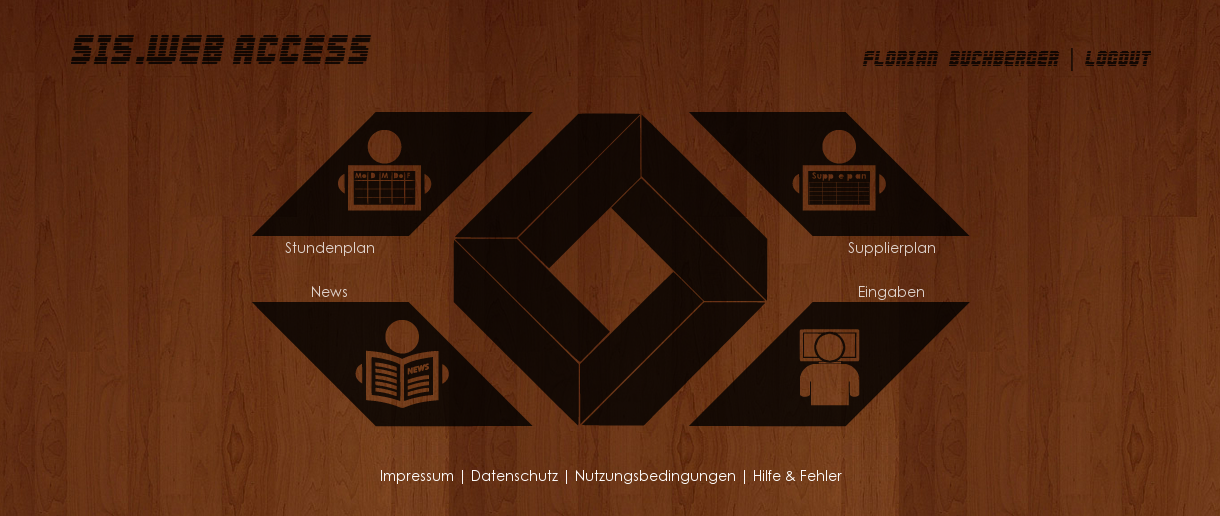
\includegraphics[keepaspectratio=true, width=14cm]{images/screenshots/web-access_nohover.png}
\caption{SIS.Web Access}
\label{fig:content_draft_design_webaccess}
\end{figure}
\begin{figure}[H]
\centering
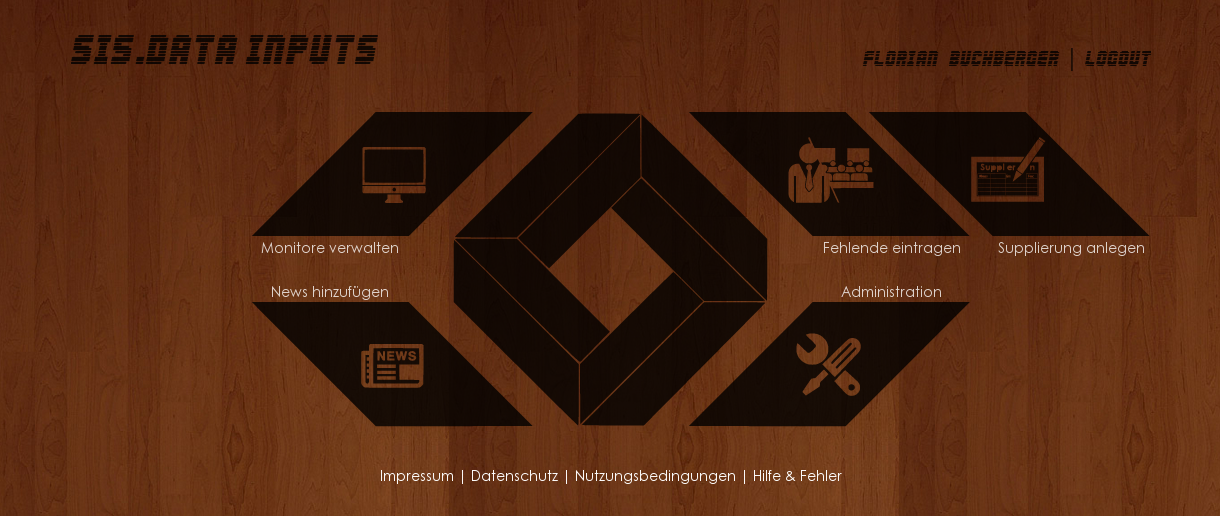
\includegraphics[keepaspectratio=true, width=14cm]{images/screenshots/data-inputs_nohover.png}
\caption{SIS.Data Inputs}
\label{fig:content_draft_design_datainputs}
\end{figure}
\begin{figure}[H]
\centering
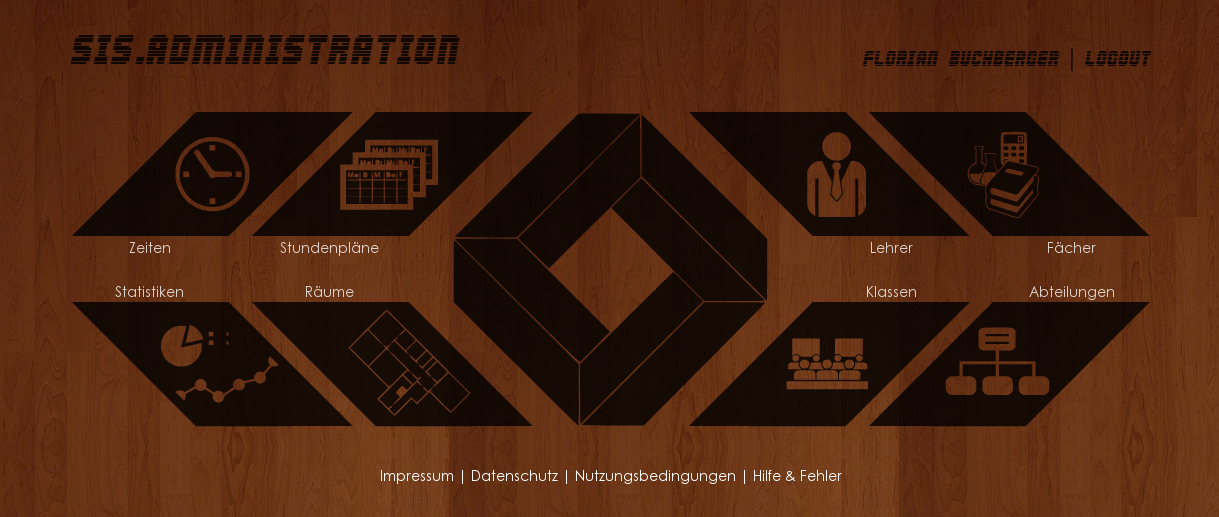
\includegraphics[keepaspectratio=true, width=14cm]{images/screenshots/administration_nohover.png}
\caption{SIS.Administration}
\label{fig:content_draft_design_administration}
\end{figure}
Mit Klick auf das Logo in der Mitte gelangt man jeweils zum vorhergehenden Menü zurück.\\
Die Buttons enthalten jeweils eine Grafik, welche den Punkt für den dieser Button steht, bestmöglich repräsentieren sollte. Ein Hoover Effekt bewirkt eine Änderung der Buttonfarbe (Schwarz auf Weiß) und weist den User daraufhin, welchen Button er aktuell gewählt hat. Dieser Effekt benötigt allerdings SVG Grafiken anstatt Beispielsweise png's, was die ganze Sache etwas kompliziert macht, dafür jedoch auch weniger Traffic – svg Grafiken sind kleiner – verursacht.\\
Da der Inhalt, welchen man erreichen soll nachdem ein Button geklickt wurde, seine Zusammengehörigkeit mit der eigentlichen Navigation/Menü nicht verlieren sollte wurde beschlossen, dass der neue Inhalt im Zuge einer Animation erscheint. Wird also ein Button angeklickt, wird der Monitor optisch quasi horizontal geteilt und auseinander geschoben. Im sich nun öffnenden Teil des Bildschirmes erscheint nun ein leicht dunklerer Hintergrund (ebenfalls Brauntöne), auf dem sich nach Beenden der Animation der Inhalt aufbaut. Um den Übergang zwischen den beiden Hintergründen sanfter zu gestalten, wurde eine weiße Linie dazwischen gezogen. Will man wieder in das Menü, kann nun entweder außerhalb des dunklen Hintergrundes auf den Bildschirm geklickt werden oder der Exit Button verwendet werden. Die Animation wird daraufhin entgegengesetzt ausgeführt und man ist wieder im ursprünglichen Menü.\\
All diese Features sind allerdings nur dann möglich, wenn Javascript aktiviert ist. Sollte das am Client PC nicht der Fall sein, wird eine Javascript-freie Seite geladen, ohne Animationen im Menü und lediglich mit der Möglichkeit, durch Anklicken des zugehörigen Buttontextes, den betreffenden Inhalt zu laden. Dieser erscheint in einem Vollbild und kann nur mit dem Exit Button wieder verlassen werden. Auf mobilen Geräten (iPhone, Android Devices usw.) wird zudem NUR die Seite ohne JS geladen, auch wenn das Device JS unterstützen würde.
\subsubsection{Monitordesign}
Die wichtigsten Inhalte, welche am Monitor angezeigt werden sind News, Supplierungen und Raumpläne. Die News werden mit weißer Schriftart in einem Schwarz transparenten Fenster mit abgerundeten Ecken angezeigt. Die Supplierungen in einer Tabelle, welche wiederum weiße Schrift auf schwarz transparentem Hintergrund ist, wobei die erste Zeile inverse Farben verwendet. Besonderheiten bei dieser Tabelle ist die Sortierung, welche nach Klassen erfolgt (vereinfacht das Lesen für die Schüler) sowie der Verzicht auf Vertikale Spaltenabtrennungen. Dies ermöglicht ein angenehmeres Lesen der Supplierungen. Die Raumbelegungspläne haben dieselbe Farbabstimmung wie der Supplierplan. Jede Zelle zeigt die drei Inhalte Klasse, Lehrer und Fach an, wobei die Klasse größer in der ersten Zeile und das Fach mit dem Lehrer in der nächsten Zeile in kleinerer Schriftart abgebildet sind.

%\section{Feinentwurf}

\section{Implementierung}

\subsection{Sourcecode}

Der vollständige Sourcecode (Stand: ) // TODO
ist auf der angehängten CD zu finden.

\subsection{Test- Und Messergebnisse}


\appendix 
% Zusätze
\chapter[Anleitungen: Benutzer]{Betriebsanleitung\\ Benutzer}
\section{Einleitung}

Dies ist die Anleitung für die Benutzung des School Information Service der HTL Anichstraße. Diese Anleitung wurde im Zuge der Diplomarbeit vom SIS-Team geschrieben, um alle Funktionen unseres Systems zu dokumentieren.

\section{Allgemein}
Nach der Anmeldung mit Benutzerdaten (dieselben wie bei moodle oder htl-wlan) erscheint das Frontend. \\
Durch einen Klick auf eines der Symbole schiebt sich, bei aktiviertem JavaScript, die Seite auseinander und der Inhalt wird angezeigt. Um zum Menü zurückzukehren kann  das Kreuz rechts oben verwendet werden. Ein Klick auf den oberen oder unteren Rand der Seite hat den gleichen Effekt.\\
Durch einen Klick auf die Schrift im linken oberen Eck oder auf das SIS-Logo in der Mitte gelangt man zum übergeordneten Menü zurück.\\
Um sich abzumelden muss \enquote{LOGOUT} in der rechten oberen Ecke angeklickt werden.\\
Ein Icon, das zwar angezeigt wird, jedoch nicht anwählbar ist, ist auf eine mangelnde Berechtigungsstufe zurückzuführen.\\
Durch Auswählen von \enquote{Fehler} wird ein Fenster geöffnet, mit dem eine E-Mail an das SIS-Team gesendet werden kann, um Fehler zu melden.\\
Zudem ist diese Anleitung unter dem Punkt Hilfe abrufbar.

\section{Stundenplan}

Um den persönlichen Stundenplan anzuzeigen, muss im Web-Interface der Punkt \enquote{Stundenplan} gewählt werden. \\
\\
Wenn die Seite aufgerufen wird, wird zunächst der modifizierte Stundenplan der aktuellen Woche angezeigt.\\

\begin{figure}[H]
\centering
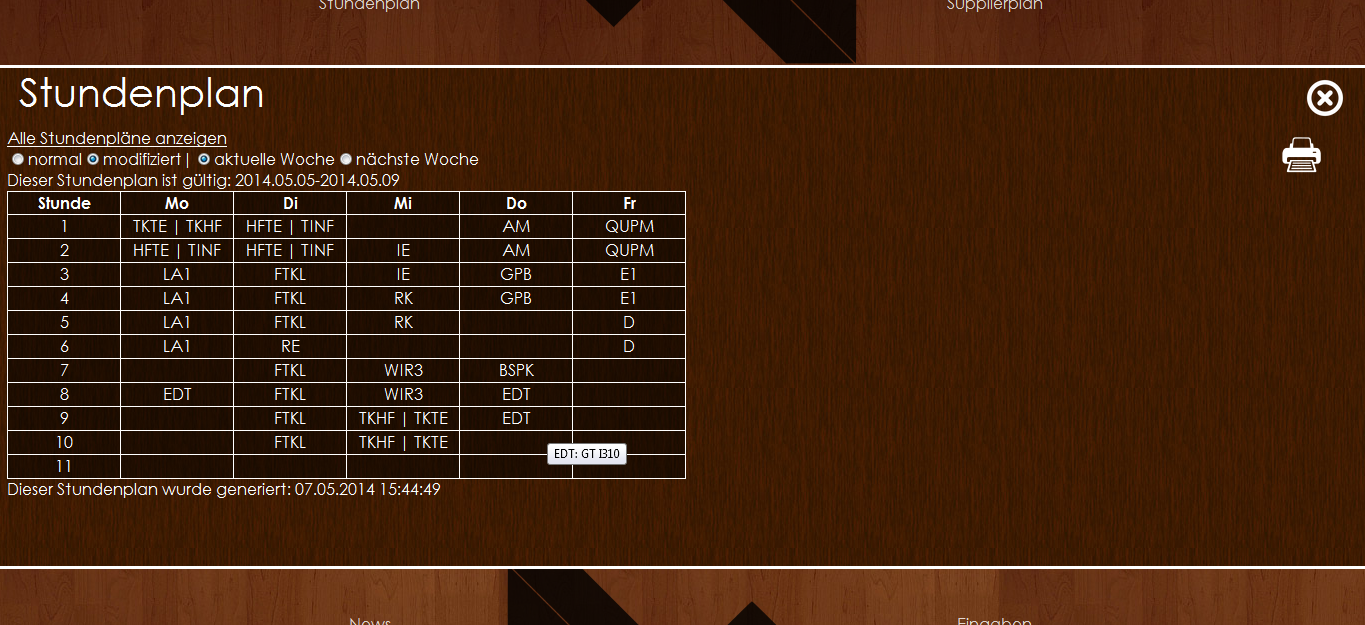
\includegraphics[keepaspectratio=true, width=14cm]{images/screenshots/timetable_mod.png}
\caption{modifizierter Stundenplan mit Popup}
\label{fig:Web_mod_timetable}
\end{figure}

Mittels der Optionen oberhalb der Stundenplanausgabe kann auf den nicht modifizierten Stundenplan umgeschalten werden. Ebenso ist es möglich den modifizierten Stundenplan der nächsten Woche anzeigen zu lassen.
Um das Popup mit den weiteren Informationen anzuzeigen, muss die Maus auf einem der Einträge platziert werden.
\subsection{modifizierter Stundenplan}
Innerhalb des modifizierten Stundenplans werden die Supplierungen der gewählten Woche angezeigt.\\
Wenn bei einer Stunde nur der Lehrer oder der Raum geändert wurde, wird im Popup der betroffene Eintrag verändert. Wenn jedoch in dieser Stunde ein anderes Fach unterrichtet wird, wird im Popup der alte Eintrag durch ein \enquote{-} ersetzt und eine zusätzliche Zeile mit dem neuen Unterrichtsgegenstand, Lehrer und Raum angezeigt.
\subsection{Stundenplan ausdrucken}
Um den eigenen Stundenplan auszudrucken, muss nur im rechten oberen Eck der Druck-Button angeklickt werden.\\
Für einen Administrator ist es zudem möglich alle anderen Stundenpläne auszudrucken. Dazu muss nur auf der Seite \enquote{Alle Stundenpläne} der Druck-Button angeklickt werden, wodurch ein PDF mit dem gerade angezeigten Stundenplan generiert wird.
\subsection{Alle Stundenpläne}
Diese Option ist nur für das Lehrpersonal und die Administration zugänglich.\\\\
Das Lehrpersonal kann nur die Stundenpläne von Klassen einsehen.\\
Beim Öffnen der Seite wird Auswahl zwischen \enquote{Lehrer} und \enquote{Klasse} und eine Eingabezeile angezeigt.\\
\\
Wenn die Option Lehrer gewählt wurde, muss in dieser Zeile das Lehrerkürzel eingegeben werden, bei der Auswahl von Klasse der Klassenname.

\begin{figure}[H]
\centering
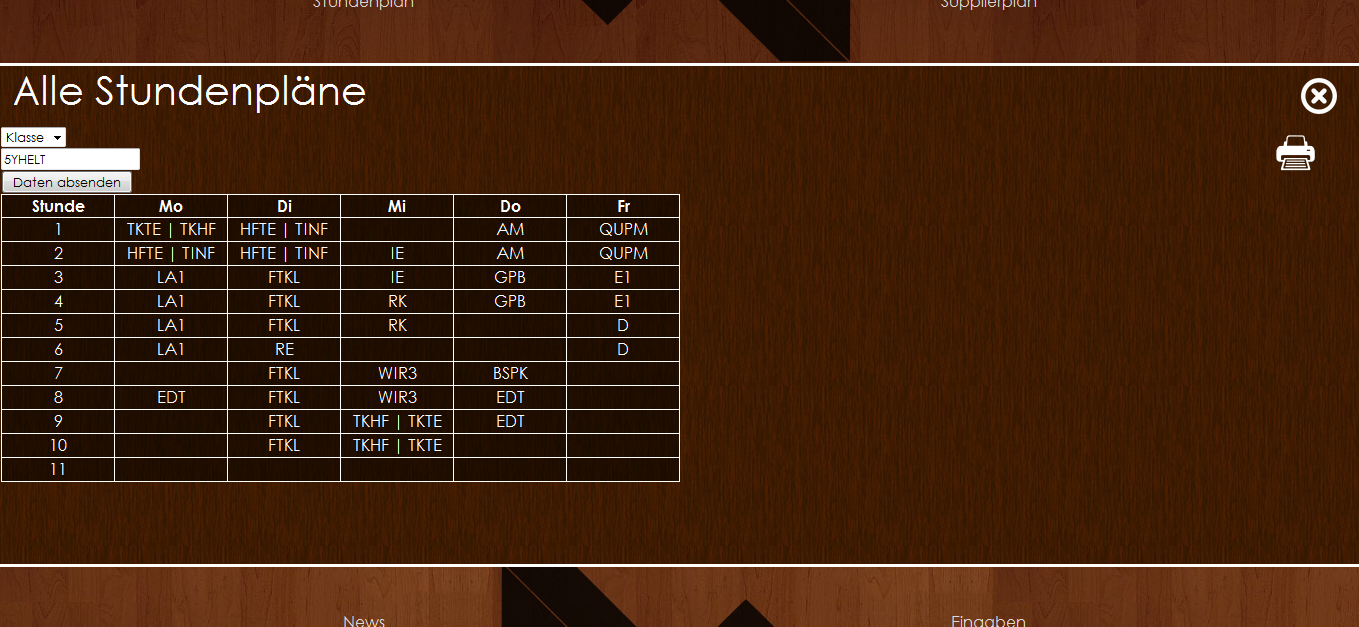
\includegraphics[keepaspectratio=true, width=14cm]{images/screenshots/timetable_all.png}
\caption{Alle Stundenpläne}
\label{fig:Web_all_timetable}
\end{figure}


\section{Supplierplan}

 Um den persönlichen Supplierplan azuzeigen, muss im Web-Interface der Punkt \enquote{Supplierplan} gewählt werden.
 \\
 \\
 Nun wird der Supplierplan für den aktuellen und den folgenden Schultag angezeigt.
 \\
 \\
 Um den Supplierplan für den übernächsten und den darauf folgenden Schultag anzuzeigen, muss der Punkt \enquote{nächste Einträge} gewählt werden.


\section{News}

 


\section{App}

\subsection{Login}
Wenn man die Applikation öffnet erscheinen zwei Eingabefelder, wobei beim oberen der Benutzername(die Novell-Schülernummer) und beim unteren das Passwort eingegeben werden muss. Der Punkt \enquote{angemeldet bleiben} kann ausgewählt werden, damit sich die Applikation beim nächsten Start selbst anmeldet. 

\subsection{Stundenplan}
\subsubsection{Angepasster Stundenplan}
Um den für den Nutzer angepassten Stundenplan zu sehen, muss man im Menü das Stundenplansymbol antippen. In diesem Stundenplan ist der Supplierplan integriert, das heißt die Stunden werden so angezeigt, wie sie wirklich gehalten werden.\\
Es gibt die Möglichkeit den angepassten Stundenplan von dieser Woche oder von der nächsten Woche anzuzeigen, dazu gibt es rechts über der Tabelle einen Button auf dem steht, \enquote{nächste Woche} bzw. \enquote{vorherige Woche}.
Um weitere Informationen zu den einzelnen Stunden zu erfahren, kann man einfach auf die gewünschte Stunde tippen, daraufhin erscheint ein Popup, in welchem das Unterrichtsfach der genutzte Raum und der Lehrer/die Klasse aufgelistet sind.

\subsubsection{Normaler Stundenplan}
Um den gewöhnlichen Stundenplan zu sehen, muss man zuerst im Menü auf das Stundenplansymbol tippen, um zum angepassten Stundenplan zu gelangen und dann muss man auf den Schriftzug \enquote{normaler Stundenp.} am unteren Ende der Seite tippen, um zum normalen Stundenplan zu gelangen.\\
Um weiter Informationen zu den einzelnen Stunden zu erfahren, siehe A.5.2.1

\subsubsection{Alle Stundenpläne}
Alle Stundenpläne (Klassenpläne) sind nur von Lehrern zu sehen. Um als Lehrer alle Stundenpläne einzusehen, muss man zuerst im Menü das Stundenplansymbol antippen, dann tippt man auf den Schriftzug \enquote{alle Stundenp.} am unteren Ende der Seite. Es erscheint ein Dropdownmenü.\\
In diesem Dropdownmenü muss man nun die Klasse auswählen, deren Stundenplan man sehen möchte und dann auf auswählen tippen. Nun erscheint der Stundenplan der ausgewählten Klasse.\\
Um weiter Informationen zu den einzelnen Stunden zu erfahren, siehe A.5.2.1

\subsection{Supplierplan}
Im Supplierplan werden alle Supplierungen die die eigene Klasse betreffen (wenn man als Lehrer angemeldet ist alle Supplierungen die einen selbst betreffen) angezeigt. Um diesen zu sehen muss man im Menü auf das Supplierplansymbol tippen.\\
Um weitere Informationen zu den einzelnen Supplierungen zu erfahren, muss man auf ein Feld in der gewünschten Zeile tippen (leere Felder funktionieren nicht). Dann erscheint ein Popup, in welchem die zu supplierende Klasse, das Fach, der supplierende Lehrer und ein Kommentar stehen.

\subsection{News}
Bei den News werden immer die Neuigkeiten, welche auch auf den Monitoren ausgeschrieben werden,  angezeigt. Um zu den News zu gelangen, muss man im Menü auf den Menüpunkt News tippen.

\chapter[Anleitungen: Administrator]{Betriebsanleitung\\ Administrator}
\section{Einleitung}

Dies ist die Anleitung für den Abteilungsvorstand bzw. Super User für das School Information Service der HTL Anichstraße. Diese Anleitung wurde im Zuge der Diplomarbeit vom SIS-Team geschrieben, um alle Funktionen unseres Systems zu dokumentieren

\newpage
\section{News}

Um die News zu bearbeiten, klicken Sie im \enquote{Data-Input-Menu} auf den Punkt \enquote{News hinzufügen}
\\
Nach dem Öffnen der Seite werden die eingetragenen News angezeigt.
\\

\subsection{News bearbeiten/hinzufügen}
\begin{description} 
\item[Titel] Titel der angezeigt werden soll.
\item[Text] Text der angezeigt werden soll.
\item[Abt.] Abteilung für welche die News angezeigt werden soll. Wenn dieses Feld leer ist, wird die News in allen Abteilungen angezeigt.
\item[Anzeigebeginn-Datum] Datum ab welchem die News angezeigt werden soll.
\item[Anzeigeend-Datum] Datum bis zu welchem die News angezeigt werden soll.
\item[Anzeigen] Zeigt an ob die News angezeigt wird. Wenn ein Newsbeauftragter eine News hinzufügt, ist dieser Punkt nicht gewählt und muss vom Abteilungsvorstand ausgewählt werden, um die News freizugeben. 
\item[Ersteller] In dieses Feld kann nichts eingegeben werden. Es dient dazu, dass der Abteilungsleiter weiß, wer die News erstellt hat.
\item[Nur Website] Wenn dieser Punkt ausgewählt ist,wird die News nur auf der Website oder in der App angezeigt und nicht auf den Monitoren.
\end{description}

\subsection{News löschen}

\newpage
\section{Monitore}

Um in die Einstellungen für die Monitore zu gelangen, klicken Sie im \enquote{Data-Input-Menü} auf den Punkt \enquote{Monitore verwalten} (siehe \autoref{fig:instr_admin_monitors_dimenu}).\\
\\
\begin{figure}[H]
\centering
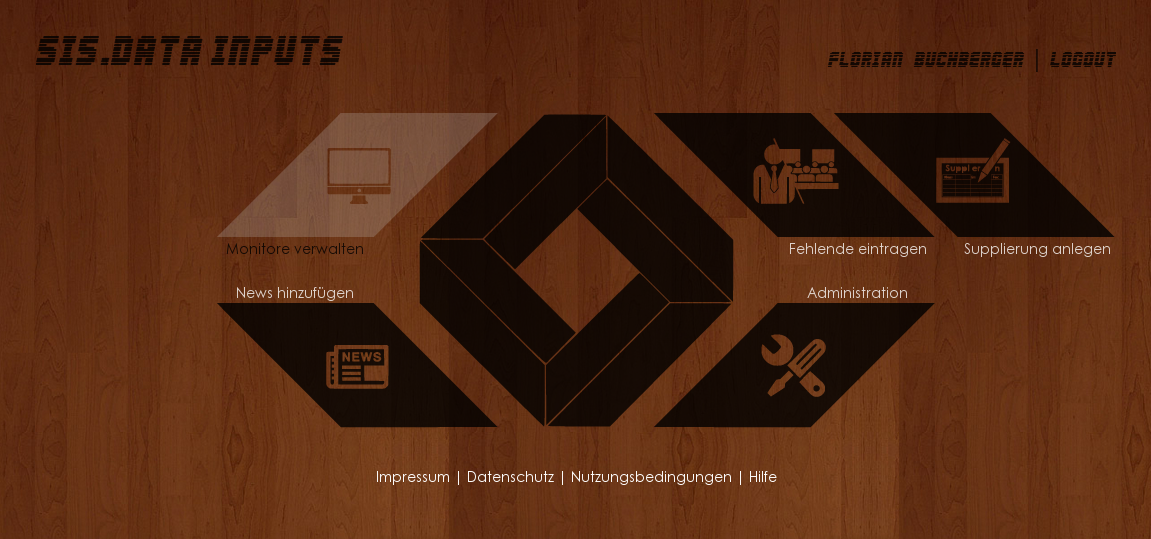
\includegraphics[keepaspectratio=true, width=14cm]{images/screenshots/data-inputs.png}
\caption{Data-Input-Menü}
\label{fig:instr_admin_monitors_dimenu}
\end{figure}
Nach dem Öffnen der Seite werden oben im Fenster die aktiven Monitore aufgelistet. Darunter sind die Einstellungen zu finden.\\
\\
\begin{figure}[H]
\centering
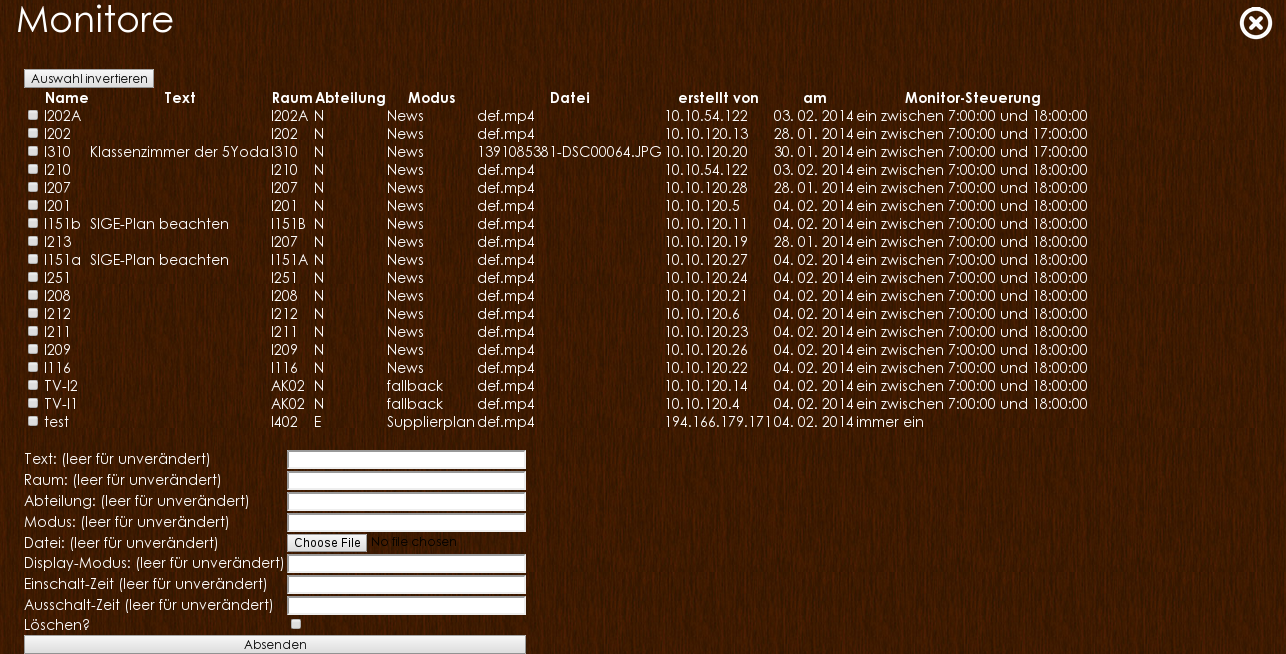
\includegraphics[keepaspectratio=true, width=14cm]{images/screenshots/monitors.png}
\caption{Monitor-Einstellungen}
\label{fig:instr_admin_monitors_site}
\end{figure}
Die Monitore, deren Einstellungen verändert werden sollen, müssen mit einem Klick auf die Checkbox links neben der Anzeige ausgwählt werden. Es können mehrere ausgewählt werden. Mit dem Button \enquote{Auswahl invertieren} werden alle gesetzten Checkbox rückgesetzt, und umgekehrt.
\\
\subsection{Hinzufügen}

\subsubsection{Software}
\label{sec:instr_monitor_software}
Für folgendes wird vorausgesetzt, dass das von uns zur Verfügung gestellte Image verwendet wird. Dieses kann unter folgender Adresse runtergeladen werden:\\ \href{https://sis.htlinn.ac.at/sis.img}{https://sis.htlinn.ac.at/sis.img}\\
Das Image ist 4 GB groß, wir empfehlen deshalb, das Image ohne Proxy-Einstellung mit der Adresse \href{http://sis.clients.htlinn.ac.at/sis.img}{http://sis.clients.htlinn.ac.at/sis.img} im Schulnetz zu laden. Das Image sollte auf eine SD-Karte mit mindestens 3965190144 Bytes Speicherplatz gespielt werden (Getestet wurde mit \enquote{SanDisk Extreme 4GB}).\\
Der vordefinierte Benutzer hat die Kennung \enquote{pi} und das Passwort \enquote{sis}.\\
\\
Ein neuer Monitor kann nicht über das Web-Interface hinzugefügt werden, die Monitore registrieren sich selbstständig am Server. Nach der Registrierung stehen sie zur Verwaltung zur Verfügung.\\
Damit sich die Monitore registrieren können, müssen sie ihre eigene Identität kennen. Diese wird in der Datei /etc/sis.conf definiert.\\

\begin{lstlisting}[style=custom,  caption={Beispiel /etc/sis.conf},label={lst:instr_admin_sisconf}]
name=test-monitor
\end{lstlisting}
Die Form des Namenseintrags ist im Beispiel  \autoref{lst:instr_admin_sisconf} ersichtlich.\\
Wenn der Name des Monitors geändert wird, sollte aus Gründen der Übersichtlichkeit und Nachvollziehbarkeit darauf geachtet werden, dass der Hostname des Raspberry Pis mit dem Namen übereinstimmt. Dazu wird die Datei /etc/hostname bearbeitet. Damit der Host nicht neu gestartet werden muss, kann mit dem Befehl \enquote{hostname} der Hostname zusätzlich auch direkt geändert werden. \\
\textit{Beispiel}: hostname I386\\
\\
\textit{Achtung:} Da es zu Problemen mit manchen Programmen (wie zum Beispiel \textit{sudo}) kommen kann, sollte in er Datei /etc/hosts ein Eintrag für den Hostnamen angelegt werden, welcher auf die lokale Adresse zeigt (üblicherweise die Loopback-Adresse 127.0.1.1).\\
\\
\textit{Achtung:} Die Software lässt es zu, dass mehrere Monitore den selben Namen tragen. Dies sollte allerdings vermieden werden.

\subsubsection{Hardware}
Die Header Platine für den Raspberry Pi wird auf demselben aufgesteckt (siehe \autoref{fig:report_hardware_Headergesteckt}). Der Monitor wird über HDMI mit dem Raspberry verbunden, die Stromversorgung ist, wie beim Raspberry üblich, mit einem USB-zu-microUSB-Adapter und einem dementsprechenden Netzteil herzustellen.\\
Als Netzwerkanbindung kann entweder die LAN-Buchse oder ein W-LAN-Stick verwendet werden. Hierbei ist zu beachten, dass der Computer, sofern er mit der unter  \autoref{sec:instr_monitor_software} beschriebenen Software betrieben wird, keine statische IP-Adresse eingetragen hat, es ist daher ein DHCP-Server notwendig. Bei Verwendung von W-LAN ist zusätzlich zu beachten, dass der Raspberry von sich aus das W-LAN \enquote{HTL-SIS} mit dem passenden WPA2-Pre-Shared-Key eingetragen hat, bei einer Änderung muss dieser angepasst werden.\\
\\
Die Verbindung zwischen dem Raspberry und der modifizierten Steckdose (siehe FTKL-Bericht) wird mit einem ausgekreuzten Mono-Klinke-Kabel hergestellt.\\
\textit{Beachte:} Wenn der Computer an die modifizierte Steckdose angeschlossen wird, dann kann er sich logischerweise nicht selbst einschalten, deshalb sollte nur der entsprechende Monitor daran angeschlossen werden.\\
\\
Sollte sich nach dem ersten Start des Computers der Monitor nicht nach spätestens 5 Minuten selbstständig einschalten, so kann es sein, dass die nicht vorhandene HDMI-Daten-Sinke den Start blockiert. In diesem Fall sollte der Monitor während dem Starten auf eine normale Steckdose gesteckt werden, läuft in dem Fall der Raspberry, so sollte die Steckdose, die Platine, sowie die Kabel überprüft und gegebenenfalls getauscht werden.

\begin{figure}[H]
\centering
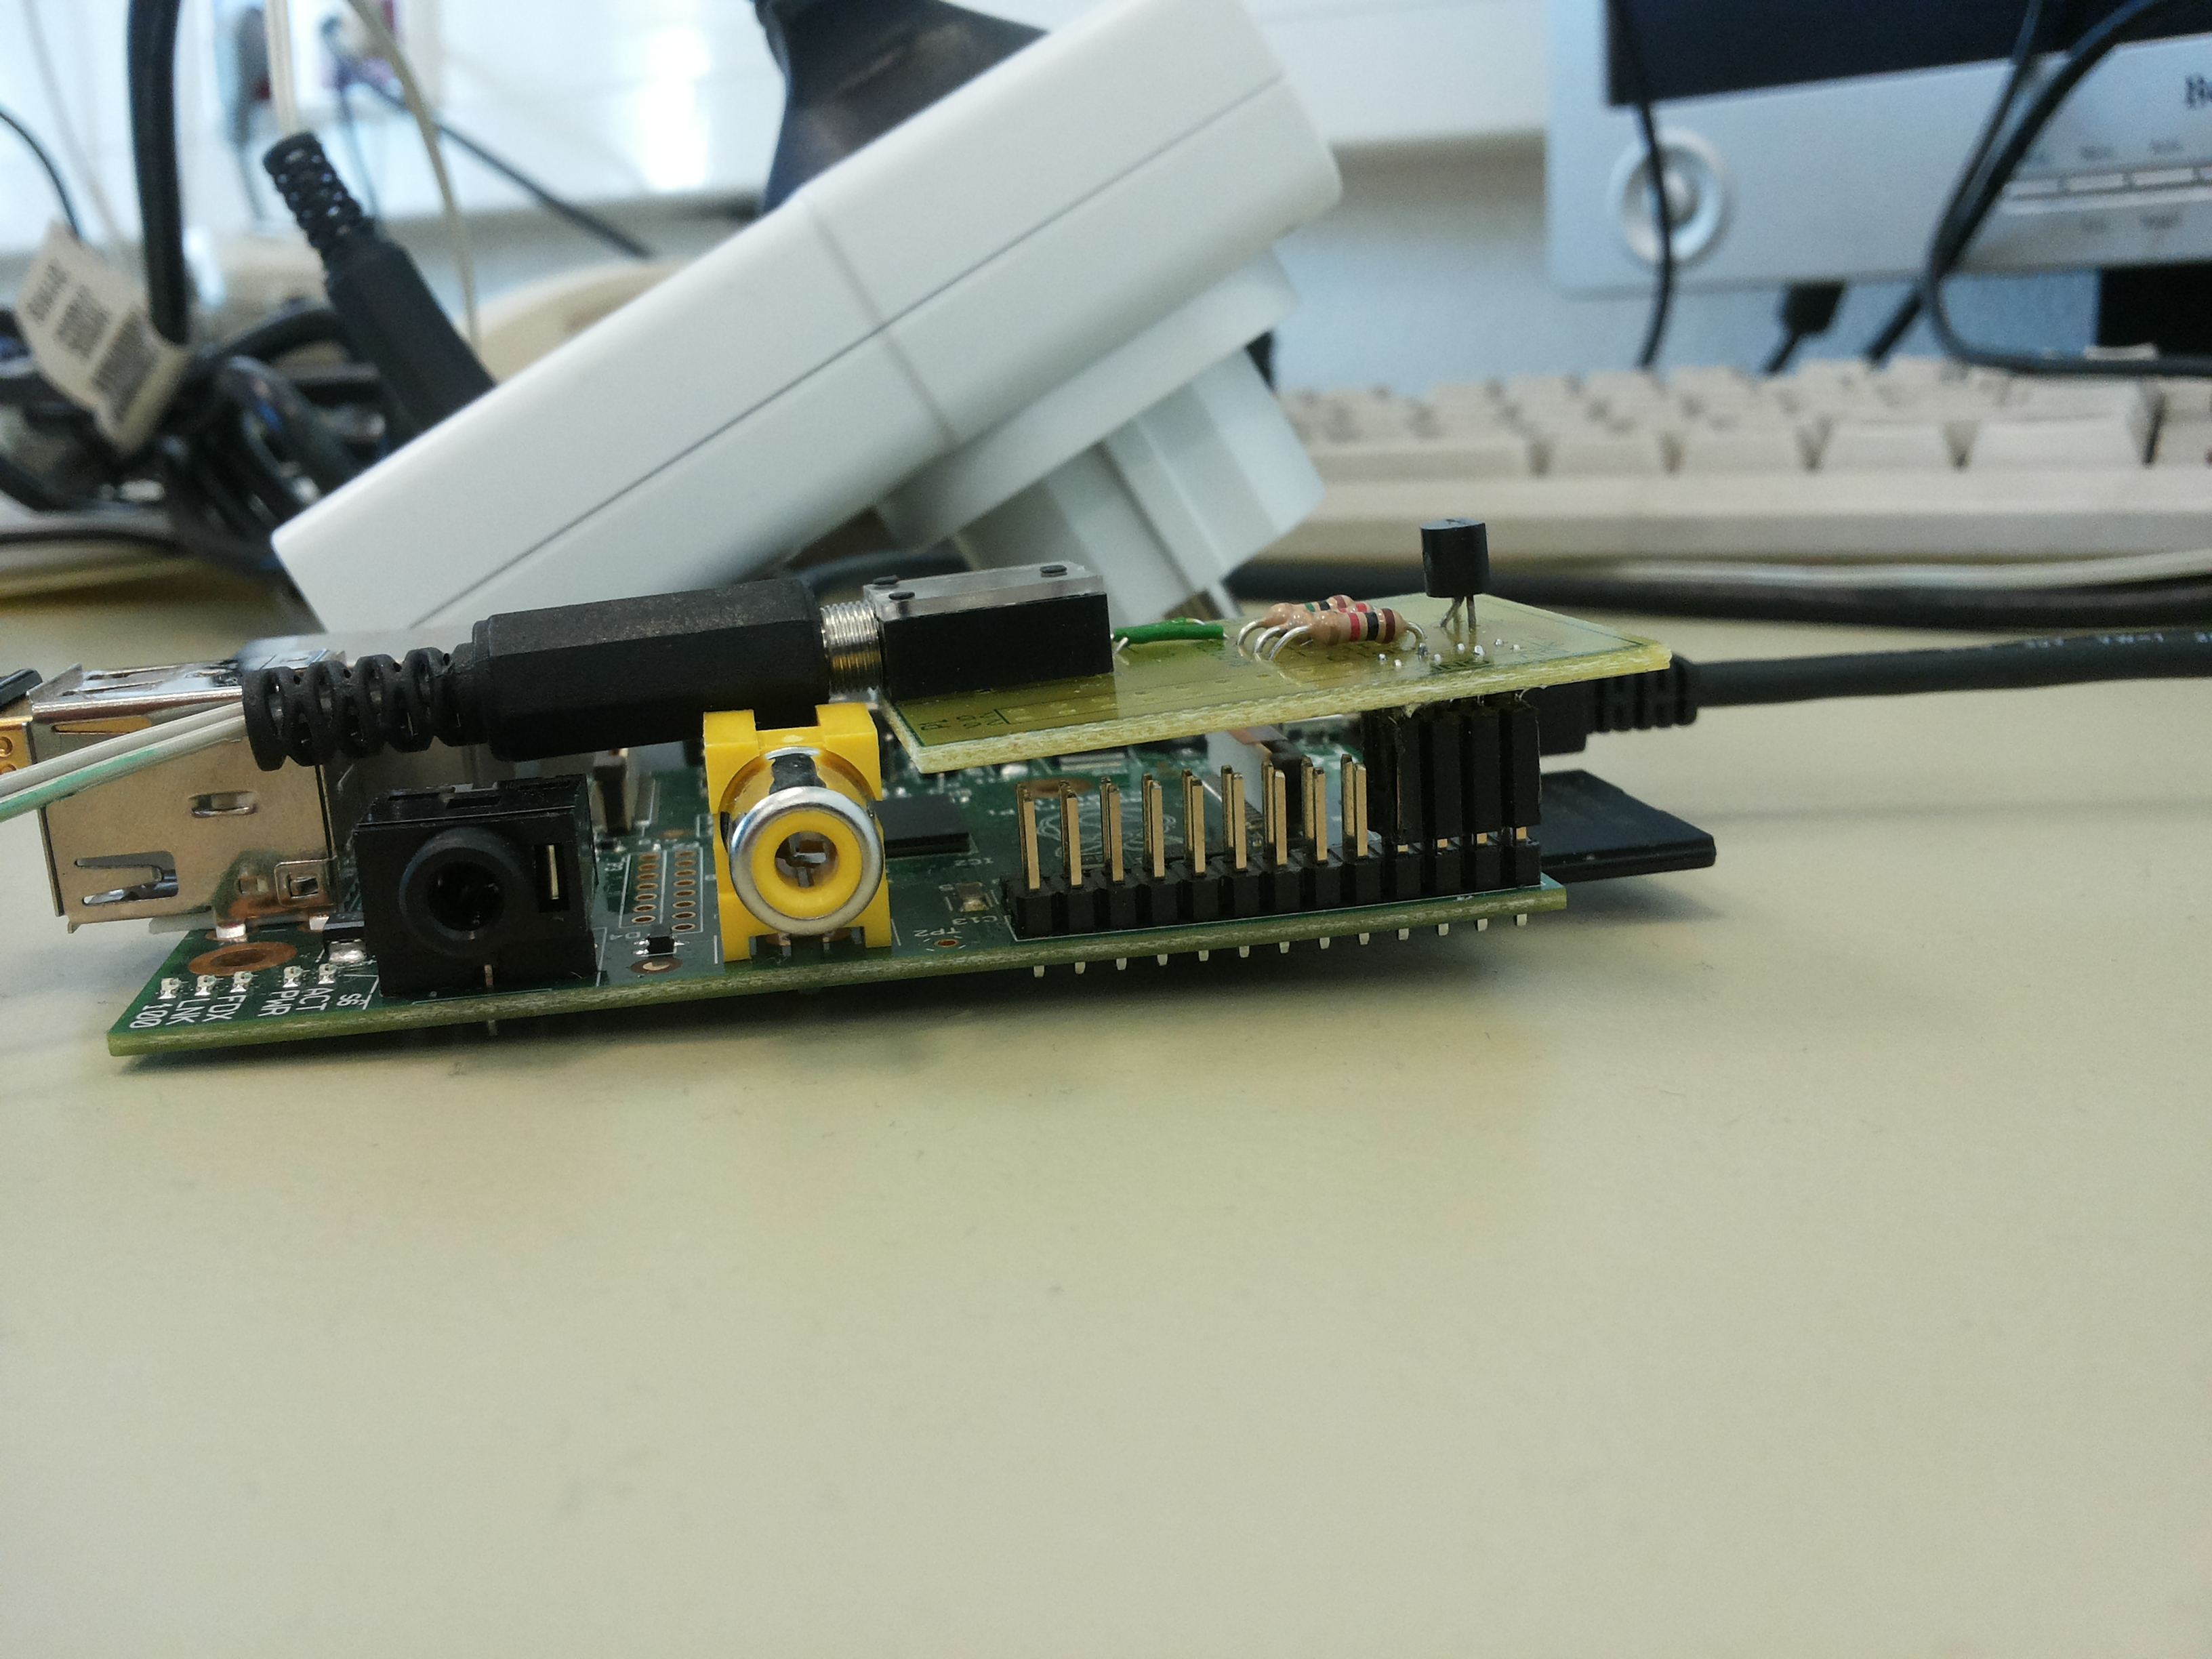
\includegraphics[keepaspectratio=true, width=10cm]{images/rpi/rpi_header_gesteckt.jpg}
\caption{Aufbau Header}
\label{fig:report_hardware_Headergesteckt}
\end{figure}

\begin{figure}[H]
\centering
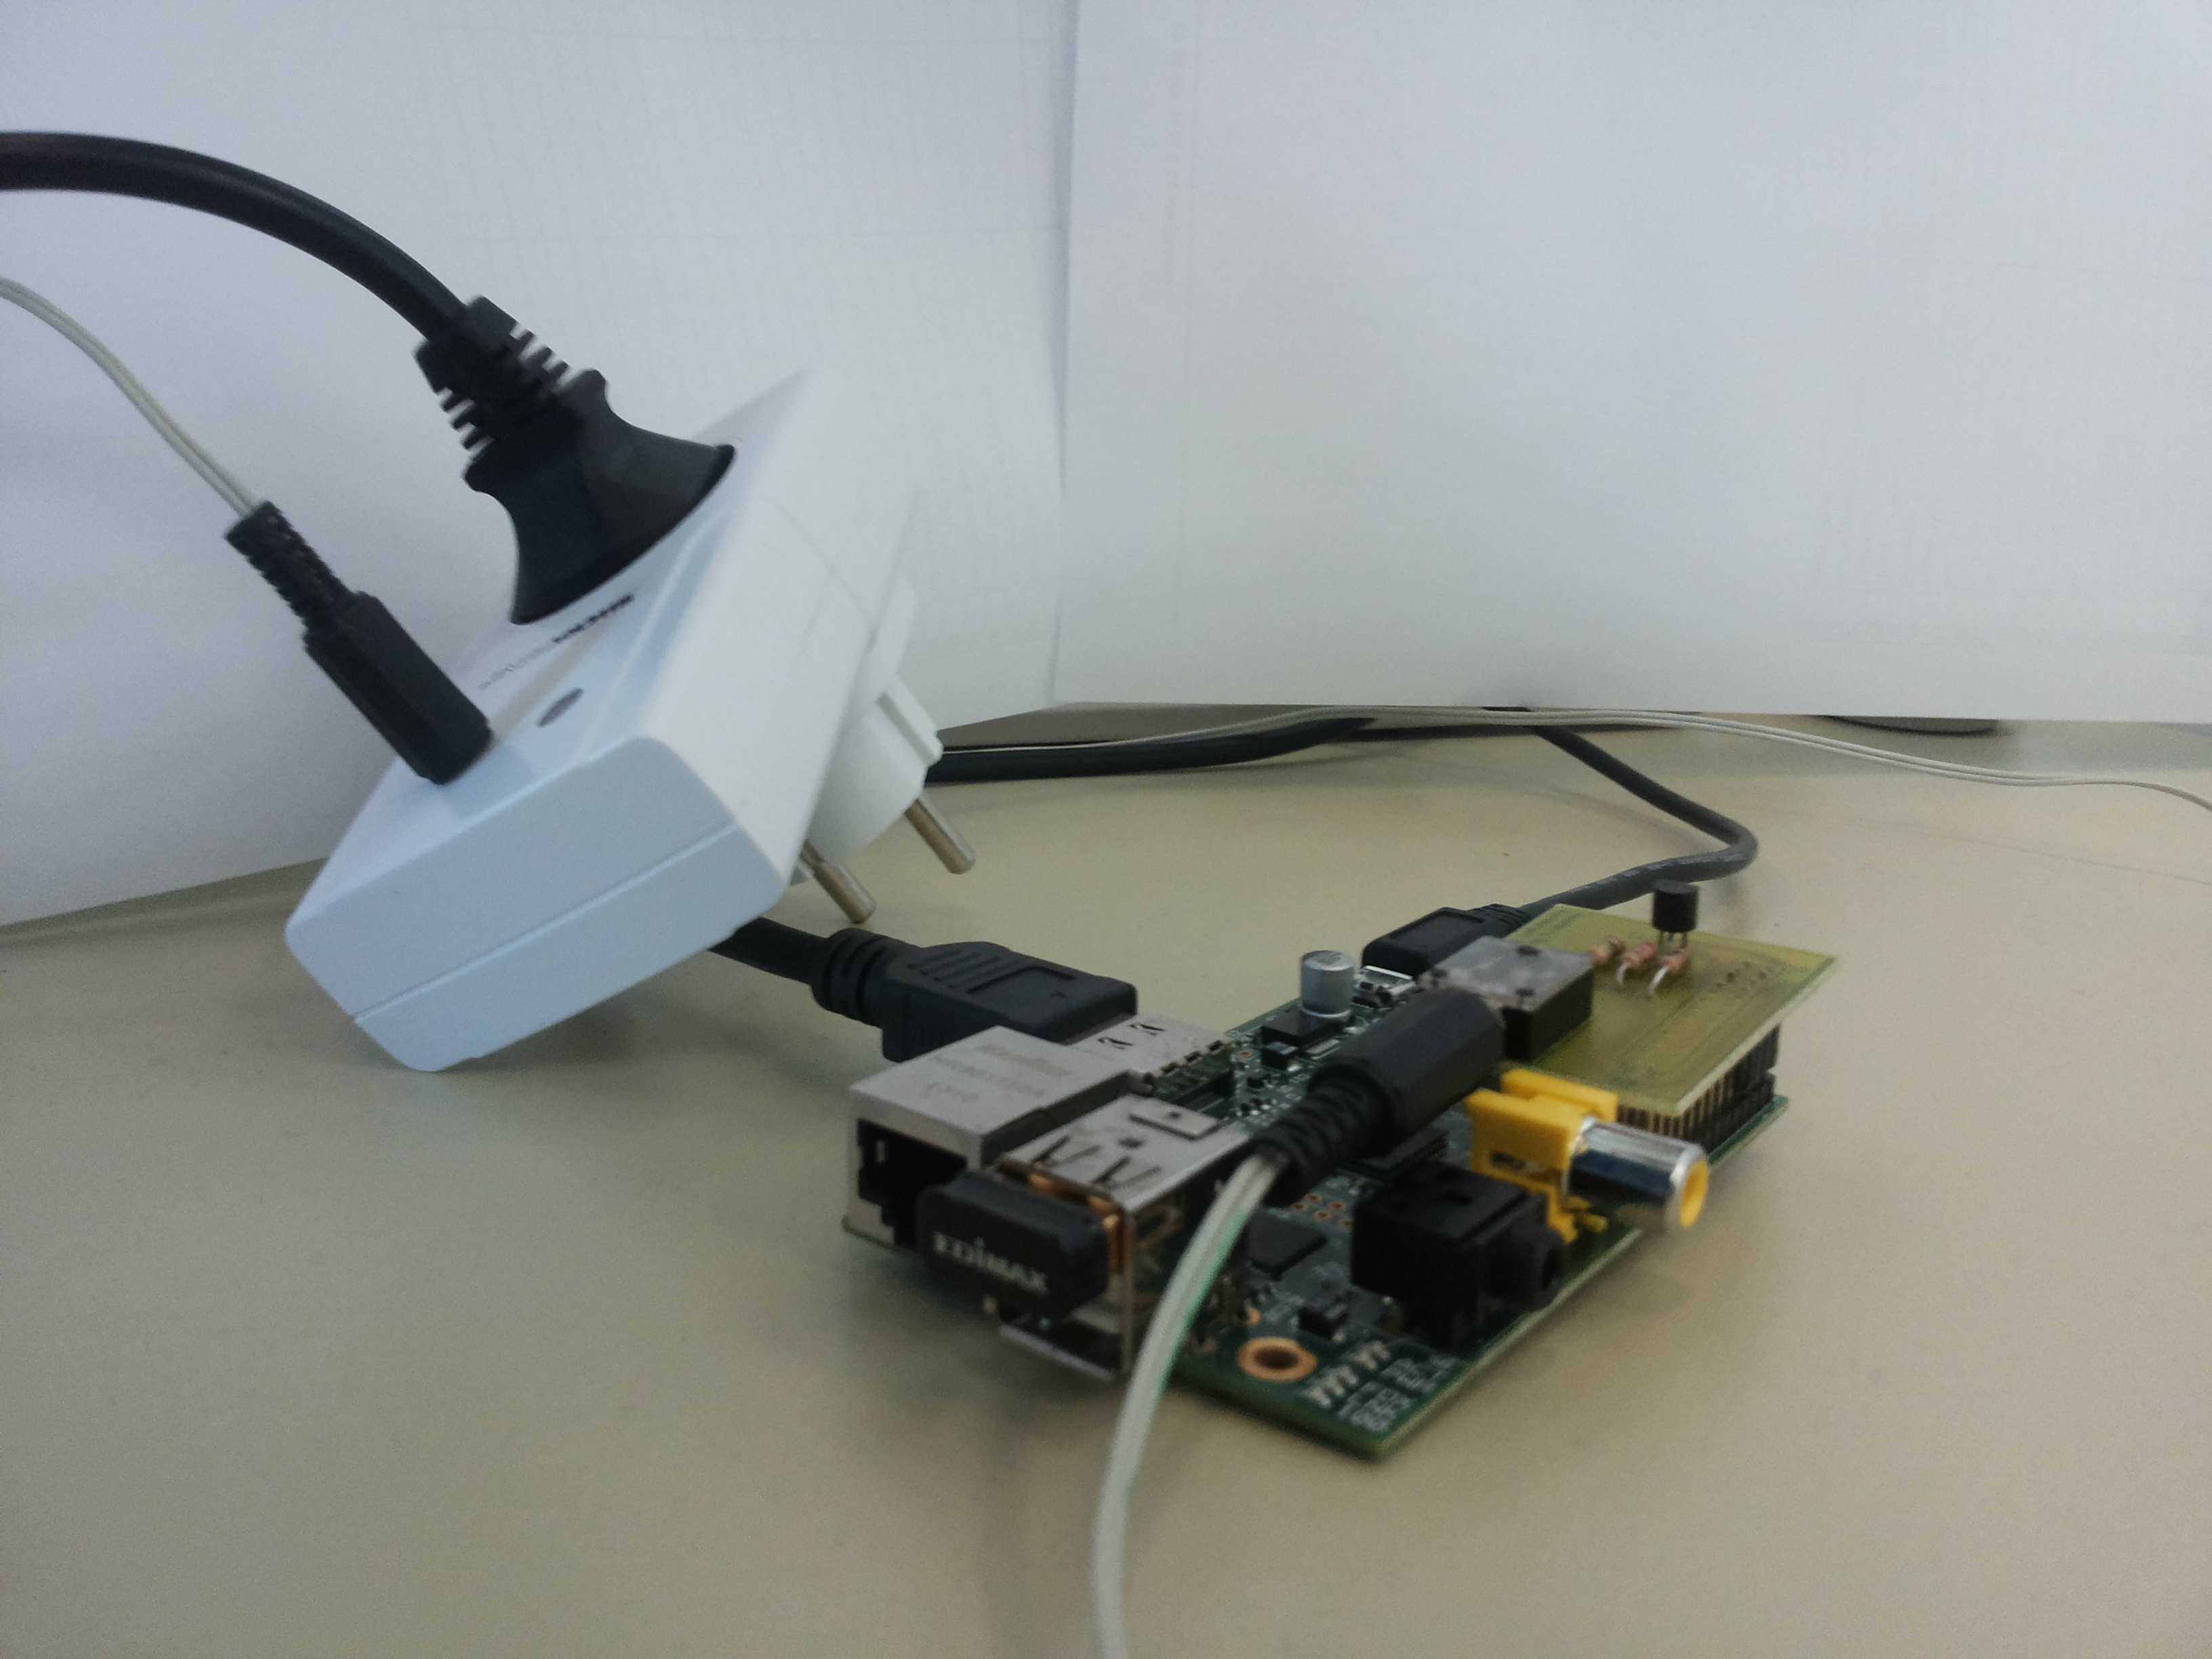
\includegraphics[keepaspectratio=true, width=10cm]{images/rpi/rpi_gesamt.jpg}
\caption{Gesamtaufbau}
\label{fig:report_hardware_Gesamt}
\end{figure}

\subsection{Entfernen}

Um einen Monitor aus der Liste der aktiven Monitore zu entfernen, wählen Sie den jeweiligen Monitor über die Checkbox aus, setzen Sie die \enquote{Löschen?}-Checkbox und klicken Sie auf \enquote{Änderungen anwenden}.\\
\\
\textit{Achtung:} Sollte der Monitor nach dem Entfernen noch eingeschalten sein, so wird sich dieser, sofern die Standard-Konfiguration eingestellt ist, wieder neu registrieren.

\subsection{Text verändern}

Der Text, der am linken unterem Eck des Monitors kann über das Eingabefeld \enquote{Text} geändert werden. Wird das Feld leer gelassen, so wird der alte Wert beibehalten.\\
\\
\textit{Achtung:} Leerzeichen werden nicht als leer erkannt.

\subsection{Raum verändern}

Für die Darstellung des Stundenplanes des jeweiligen Raumes wird jedem Monitor ein Raum zugeordnet. Diese Einstellung kann über das Eingabefeld \enquote{Raum} angepasst werden. Durch Doppelklick auf das Eingabefeld öffnet sich - sofern der verwendete Browser diese Funktion unterstützt - ein Menü, in dem durch Eingeben gesucht werden kann. Wird das Feld leer gelassen, so wird der alte Wert beibehalten.

\subsection{Abteilung verändern}

Die News können Abteilungen zugeordnet werden. Ebenso ist der Supplierplan für jede Abteilung anders. Als Folge daraus gibt es eine Einstellungsmöglichkeit für die Abteilung. Durch Doppelklick auf das Eingabefeld öffnet sich - sofern der verwendete Browser diese Funktion unterstützt - ein Menü, in dem durch Eingeben gesucht werden kann. Wird das Feld leer gelasen, so wird der alte Wert beibehalten.

\subsection{Modus verändern}

Um die ausgewählten Monitore auf Supplierplan, Stundenplan, News etc. umzuschalten, wird das Eingabefeld \enquote{Modus} verwendet. In diesem Feld sind folgende Werte zulässig:
\begin{itemize}
	\item News
	\item Stundenplan
	\item Supplierplan
	\item Supplierplan \& News
	\item Bild
	\item (Video)
	%\item (fallback)
\end{itemize}
Durch Doppelklick auf das Eingabefeld öffnet sich - sofern der verwendete Browser diese Funktion unterstützt - ein Menü mit den möglichen Werten. Wird das Feld leer gelassen, so wird der alte Wert beibehalten.\\
\\
Der Modus \enquote{Video} ist zwar implementiert, allerdings ist der Raspberry Pi nicht in der Lage, die Videos wiederzugeben.\\
%Der Modus \enquote{fallback} fährt den Monitor auf das FTKL-Schnitzel-Suppla-Projekt.\\ 
%\textit{Achtung:} Es ist nicht über das Web-Interface möglich, den Monitor wieder auf das SIS-Projekt zurückzuholen.

\subsection{Datei verändern}

Für die Modi \enquote{Bild} und \enquote{Video} muss eine Datei hochgeladen werden, welche dann angezeigt wird.\\ 
Unterstützte Dateitypen sind:
\begin{itemize}
	\item JPG, JPEG
	\item PNG
	\item GIF
	\item MP4, MPEG
\end{itemize}
Die maximale Dateigröße ist limitiert durch:
\begin{itemize}
	\item das Upload-Script auf 800 MB
	\item den Upload-HTML-Tag auf 800 MB
	\item die PHP-Konfiguration am Server (Stand: 2014-02-28) auf 128 MB
\end{itemize}
Wird das Feld leer gelassen, so wird der alte Wert beibehalten.\\

\subsection{Display-Modus verändern}

Die Raspberry Pis verfügen über einen Mechanismus, um den angeschlossenen Monitor ein- bzw auszuschalten.\\
Es sind folgende Modi möglich:
\begin{itemize}
	\item permanent Ein
	\item permanent Aus
	\item automatisch
\end{itemize}
Im automatischen Modus werden die Einstellungen von \ref{instr_admin_moni_time_on} und \ref{instr_admin_moni_time_off} verwendet.\\
\\
Wird das Feld leer gelassen, so wird der alte Wert beibehalten.\\

\subsubsection{Einschalt-Zeit}
\label{instr_admin_moni_time_on}

Bestimmt die Zeit, an dem sich der angeschlossene Monitor einschalten soll.\\
\textit{Beispiele:}
\begin{tabbing}
\hspace{2cm}\=\kill
7 \> 7 Uhr früh\\ 
6:35 \> 6:35 früh\\
17:05:11 \> 5:05:11 nachmittags
\end{tabbing}
Wird das Feld leer gelassen, so wird der alte Wert beibehalten.\\

\subsubsection{Ausschalt-Zeit}
\label{instr_admin_moni_time_off}

Analog zu \ref{instr_admin_moni_time_on}.


\newpage
\section{Fehlende}\label{sec:instr_admin_absentees}

Im Menü \enquote{Data-Input} (siehe \autoref{fig:instr_admin_absentees_dimenu}) können über den Auswahlpunkt \enquote{Fehlende eintragen}  fehlende Lehrer und fehlende Klassen eingegeben werden. Es öffnet sich ein weiteres Menü (siehe \autoref{fig:instr_admin_absentees_menu}) mit der Wahlmöglichkeit zwischen Lehrer und Klassen.
\begin{figure}[H]
\centering
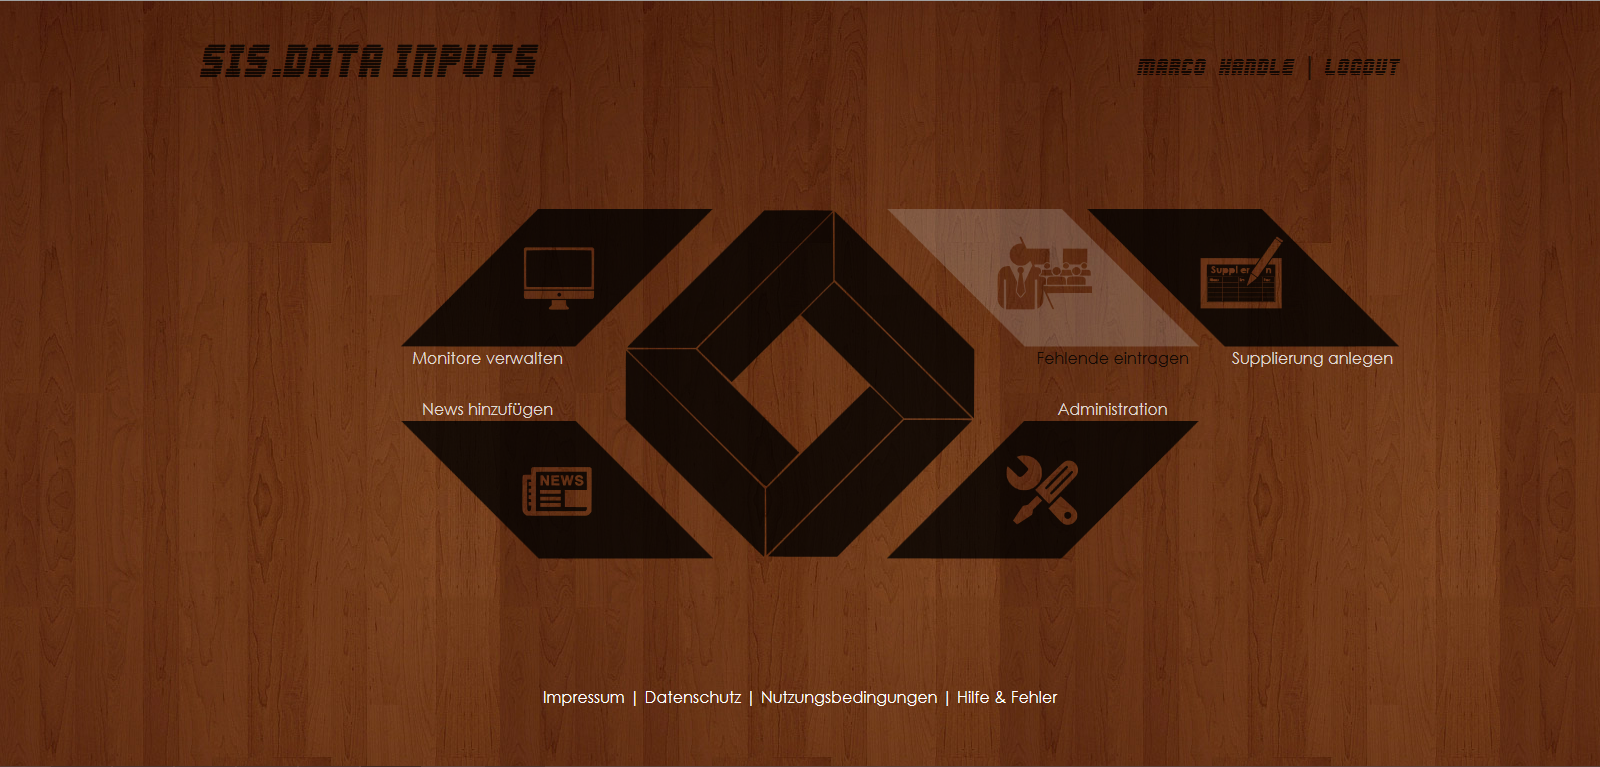
\includegraphics[keepaspectratio=true, width=14cm]{images/screenshots/data-inputs2.png}
\caption{Data-Input-Menü}
\label{fig:instr_admin_absentees_dimenu}
\end{figure}
\begin{figure}[H]
\centering
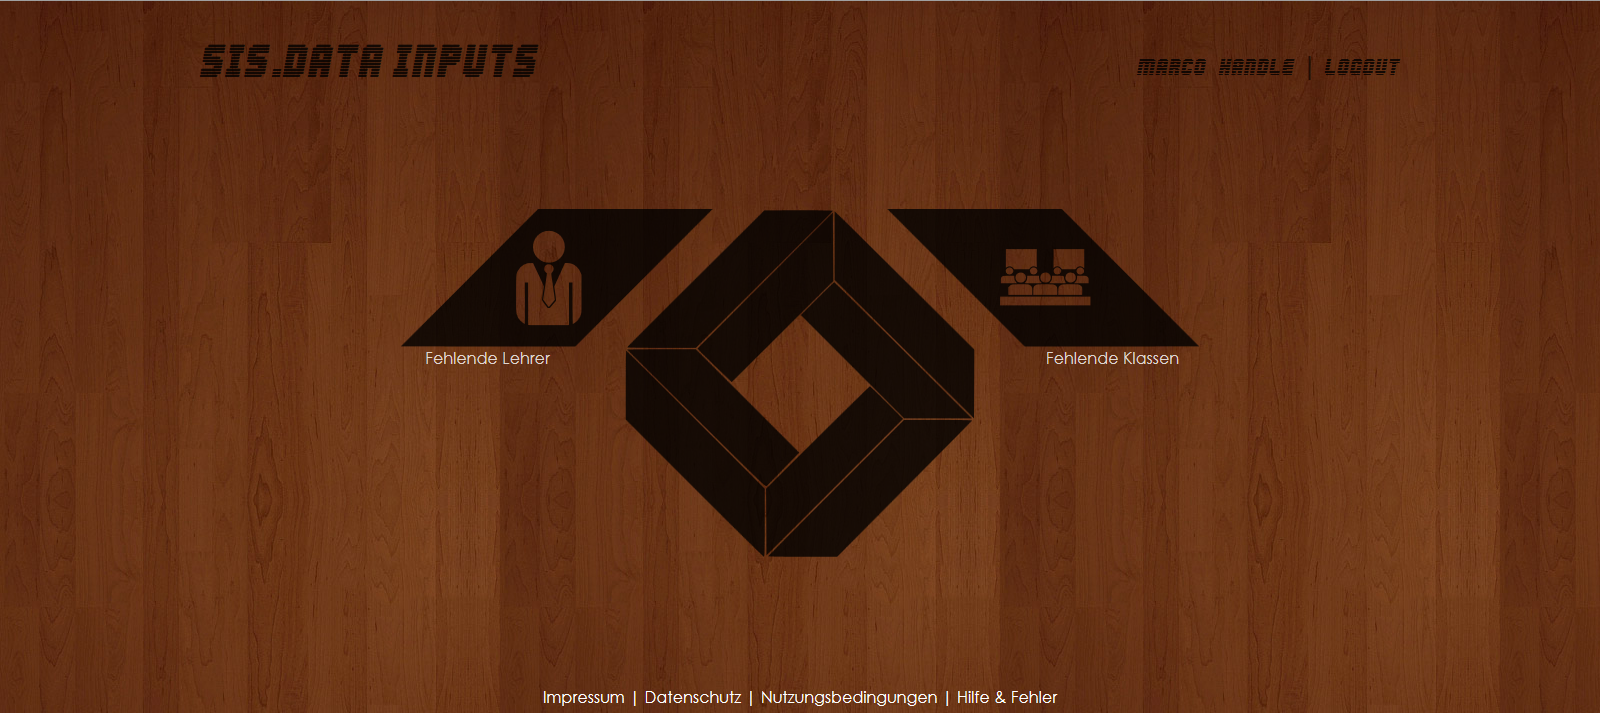
\includegraphics[keepaspectratio=true, width=14cm]{images/screenshots/data-inputs_absentees.png}
\caption{Fehlende Auswahl}
\label{fig:instr_admin_absentees_menu}
\end{figure}
\subsection{Fehlende Lehrer}
\label{sec:instr_admin_absentees_teacher}
In der tabellarischen Eingabemaske (siehe \autoref{fig:instr_admin_absentees_Lehrer}) können nun fehlende Lehrer hinzugefügt, Einträge geändert oder gelöscht werden. Standardmäßig werden beim Öffnen der Eingabemaske die für den aktuellen Tag erfassten Fehlenden Lehrer angezeigt.
\subsubsection{Fehlenden Lehrer Hinzufügen} \label{sec:instr_admin_absentees_teacher_insert}
Als erster Schritt ist das Datum des Tages auszuwählen, für den fehlende Lehrer erfasst werden. Dies kann entweder durch das Vor- und Zurückblättern mit den Pfeiltasten erfolgen oder durch eine manuelle Eingabe (Format yyyy-mm-dd). Die manuelle Eingabe ist mit der Enter-Taste zu bestätigen. Dieses Datum wird in neuen Eingabezeilen automatisch in das Feld Starttag eingetragen. Dann sind die einzelnen Eingabefelder zu befüllen.\\
\begin{table}
\centering
\begin{tabular}{p{3 cm}p{6 cm}p{5 cm}}
   \toprule
   \textbf{Eingabefeld} & \textbf{Typ} & \textbf{Wertebereich} \\
   \midrule
          \textbf{Lehrer} & Text \newline Kürzel des Lehrers -Auswahl aus Listenfeld & \\
          \hline
          \textbf{Starttag} & Datum \newline Wird automatisch eingetragen und kann nicht verändert werden &  \\
          \hline
          \textbf{Start-Stunde} & nummerisch & 1-16\\
          \hline
          \textbf{Endtag} & Datum \newline Standardmäßig wie Starttag ist auf gewünschtes Datum zu ändern & Größer oder gleich Starttag und kein Samstag oder Sonntag \\
          \hline
          \textbf{End-Stunde} & nummerisch & 1-16 \newline Wenn Starttag und Endtag gleich, dann größer als Start-Stunde\\
          \hline
          Grund & Text - optional \newline Freie Texteingabe für den Grund des Fehlens & \\
   \bottomrule
\end{tabular}
\caption{Eingabefelder Fehlende}
\end{table}
Sind alle Pflicht-Eingabefelder befüllt, wird durch Drücken auf Übernehmen die Eingabezeile übernommen, wobei vorher eine Plausibilitätsüberprüfung vorgenommen wird. Sollte eine Fehleingabe bemerkt werden, wird in einem Popup-Fenster (siehe \autoref{fig:instr_admin_absentees_fail}) das fehlerhafte Feld angezeigt. Die Eingabefelder werden gelöscht und müssen neu erfasst werden. Bei einer fehlerfreien Übernahme wird in der Eingabezeile die Checkbox Löschen und eine weitere Eingabezeile angezeigt.
\subsubsection{Eingabezeile verändern}
Ein bereits übernommener Eintrag kann noch nachträglich verändert werden. Die Änderungen sind in den Feldern vorzunehmen und dann wie unter \autoref{sec:instr_admin_absentees_teacher_insert} für jede Eingabezeile zu übernehmen.
\subsubsection{Eingabezeile löschen}
Das Löschen eines fehlenden Lehrers erfolgt über die Checkbox \enquote{Löschen} der entsprechenden Eingabezeile. Diese muss ausgewählt werden und dann mit Übernehmen bestätigt werden. Es erfolgt keine weitere Sicherheitsabfrage und der Eintrag ist \textbf{unwiderruflich} gelöscht (siehe \autoref{fig:instr_admin_absentees_Leherer_delete}).
\begin{figure}[H]
\centering
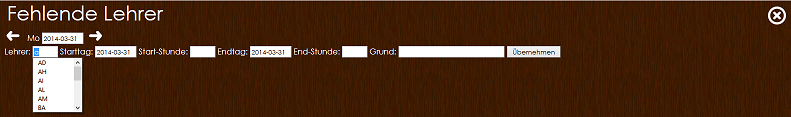
\includegraphics[keepaspectratio=true, width=16cm]{images/screenshots/absentees_teacher.png}
\caption{Fehlende Lehrer}
\label{fig:instr_admin_absentees_Lehrer}
\end{figure}
\begin{figure}[H]
\centering

\includegraphics[keepaspectratio=true, width=4cm]{images/screenshots/input_fail_teacher.png}
\caption{Falsche Eingabe}
\label{fig:instr_admin_absentees_fail}
\end{figure}
\begin{figure}[H]
\centering

\includegraphics[keepaspectratio=true, width=16cm]{images/screenshots/absentees_teacher_delete.png}
\caption{Fehlenden Lehrer löschen}
\label{fig:instr_admin_absentees_Leherer_delete}
\end{figure}
\subsection{Fehlende Klassen}
Die Erfassung von Fehlenden Klassen erfolgt analog jener der Fehlenden Lehrer. Die Eingabemenüs und Eingabefelder sind sinngemäß wie unter \autoref{sec:instr_admin_absentees_teacher} beschrieben zu verwenden.

\newpage
\section{Supplierungen}

Das Erfassen von Supplierungen kann im Menü \enquote{Data Input} gestartet werden (siehe \autoref{fig:instr_substitudes_dataInput}). Es wird die Eingabemaske für die Abteilung des Users geöffnet (siehe \autoref{fig:instr_substitudes_subNoFree}). Der Super-User muss zuerst die zu bearbeitende Abteilung auswählen (siehe \autoref{fig:instr_substitudes_subSuUs}).
\begin{figure}[H]
\centering
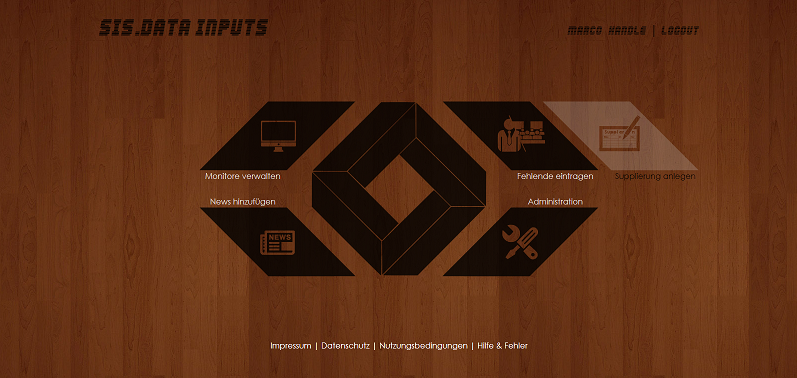
\includegraphics[keepaspectratio=true, width=17cm]{images/screenshots/data-inputs_substitudes.png}
\caption{Data-Input-Menü}
\label{fig:instr_substitudes_dataInput}
\end{figure}
\begin{figure}[H]
\centering
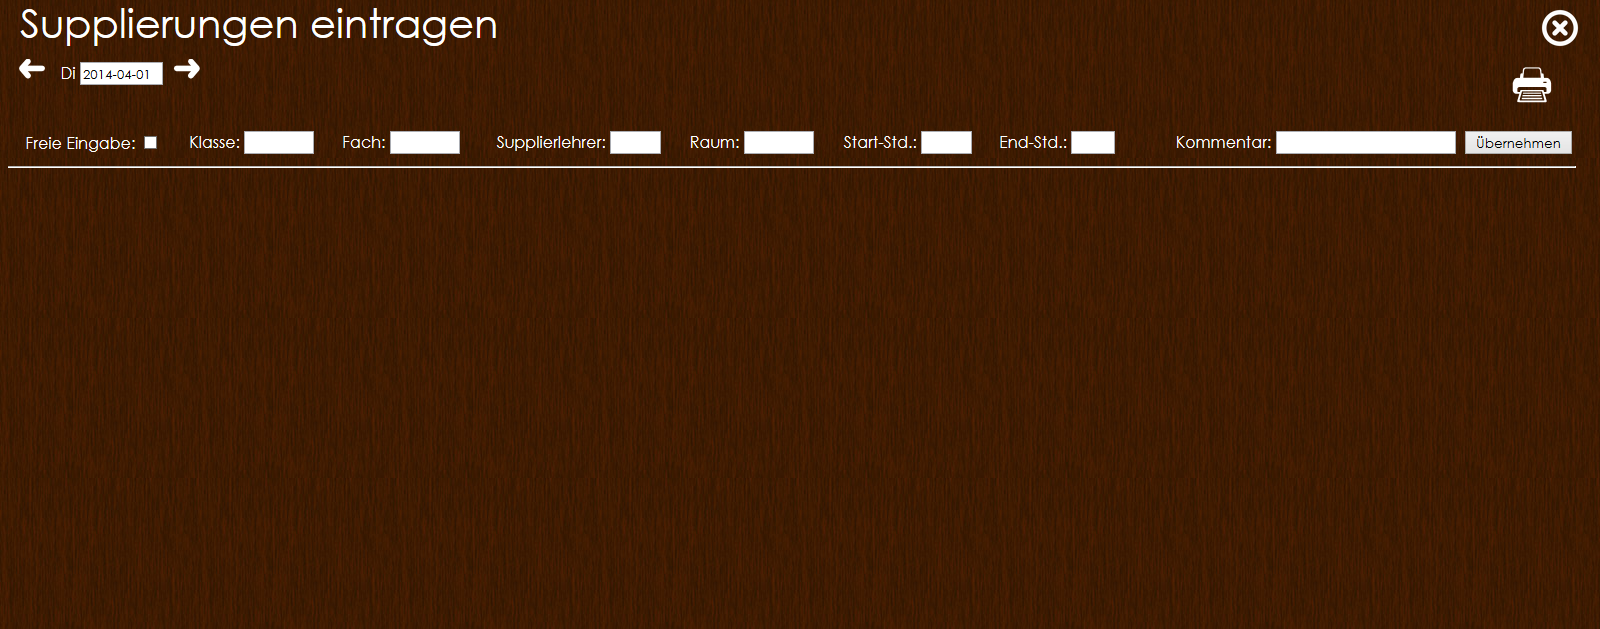
\includegraphics[keepaspectratio=true, width=17cm]{images/screenshots/substitudes_nofree.png}
\caption{Eingabemaske normal}
\label{fig:instr_substitudes_subNoFree}
\end{figure}
\begin{figure}[H]
\centering
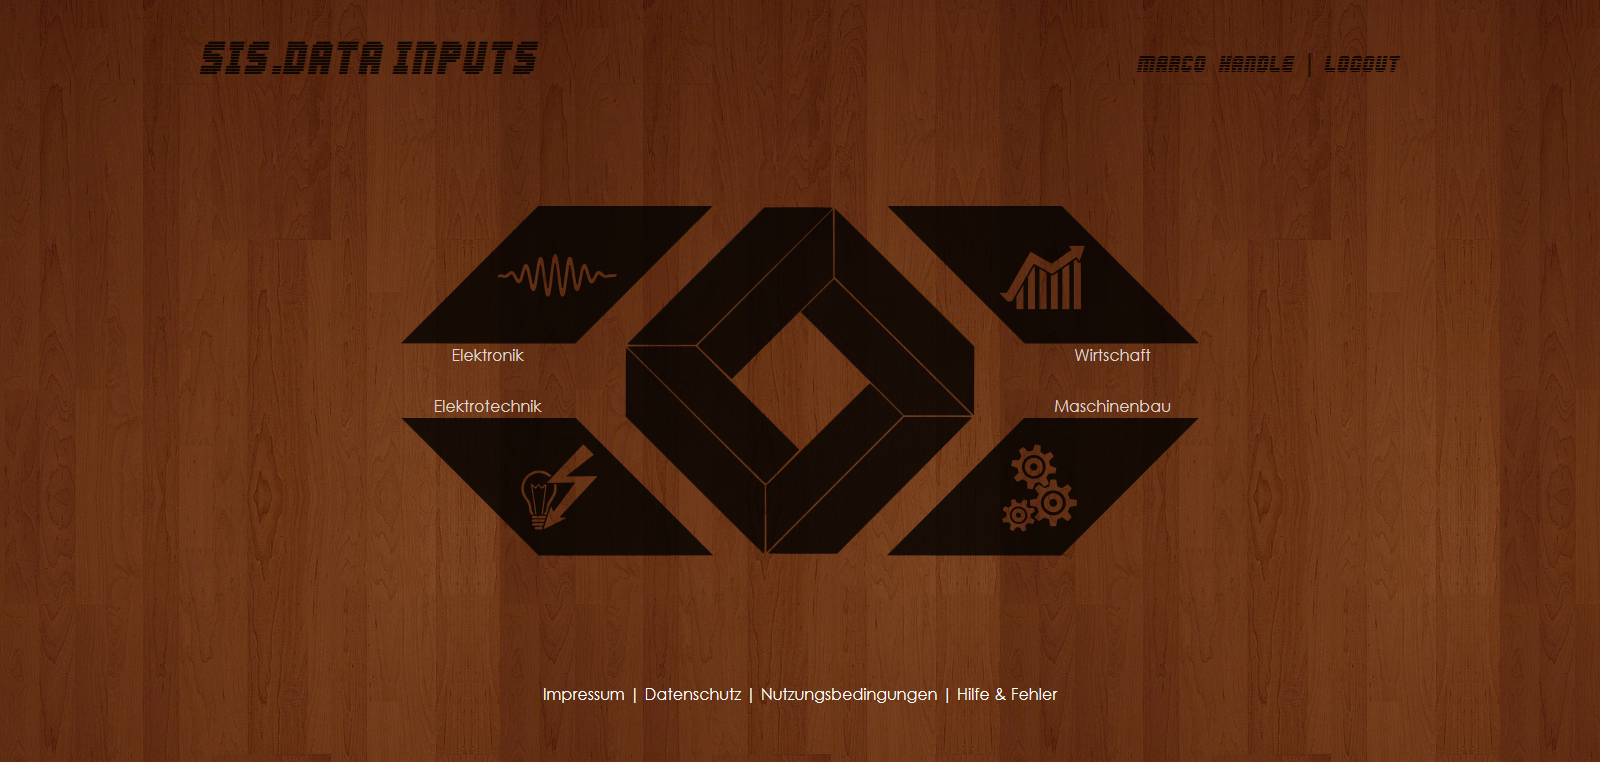
\includegraphics[keepaspectratio=true, width=17cm]{images/screenshots/substitudes_sections.png}
\caption{Super User Auswahl}
\label{fig:instr_substitudes_subSuUs}
\end{figure}
Es gibt 4 grundlegende Eingabevarianten:
\begin{itemize}
	\item Normale Eingabe\\
		siehe \autoref{sec:instr_admin_sub_noFree}
	\item Freie Eingabe\\
		siehe \autoref{sec:instr_admin_sub_Free}
		\begin{itemize}
			\item Stunde verschieben\\
				siehe \autoref{sec:instr_admin_sub_move}
			\item Stunde hinzufügen\\
				siehe \autoref{sec:instr_admin_sub_add}
			\item Stunde entfällt\\
				siehe \autoref{sec:instr_admin_sub_remove}
		\end{itemize}
\end{itemize}
\subsection{Normale Eingabe}\label{sec:instr_admin_sub_noFree}
Diese Eingabemethode (siehe \autoref{fig:instr_substitudes_subNoFree}) dient zur Erfassung von Supplierstunden von Klassen, deren Lehrer vorher als fehlend definiert wurde. Fehlen mehrere Lehrer in einer Klasse zur selben Zeit (Labor, FTKL, ...) ist die Freie Eingabe (siehe \autoref{sec:instr_admin_sub_Free}) zu verwenden.
\begin{table}[H]
\centering
\begin{tabular}{p{3 cm}p{6 cm}p{5 cm}}
   \toprule
   \textbf{Eingabefeld} & \textbf{Typ} & \textbf{Wertebereich} \\
   \midrule
          Freie Eingabe & Checkbox \newline nicht genutzt & \\
          \hline
          \textbf{Klasse} & Listenfeld - Pflichtfeld & Abteilungs-abhängig \\
          \hline
          Fach & Listenfeld - optional & \\
          \hline
          \textbf{Supplierlehrer} & Listenfeld - Pflichtfeld & \\
          \hline
          Raum & Listenfeld - optional & \\
          \hline
          \textbf{Start-Std.} & Erste Schulstunde der Supplierung  -Pflichtfeld & 1-16 \\
		  \hline
          \textbf{End-Std.} & Letzte Schulstunde der Supplierung  -Pflichtfeld & 1-16 \newline größer oder gleich Start-Std.\\
          \hline
          Kommentar & Textfeld - optional & \\
   \bottomrule
\end{tabular}
\caption{Eingabefelder normale Eingabe}
\end{table}
Mit der Schaltfläche Übernehmen wird eine Plausibilitätsüberprüfung vorgenommen und bei fehlerfreier Eingabe die Supplierstunde übernommen. Bei einer Fehleingabe wird der Fehler angezeigt und muss korrigiert werden. Nach der korrekten Übernahme wird die Checkbox Löschen in der erfassten Eingabezeile eingeblendet.
\subsection{Freie Eingabe} \label{sec:instr_admin_sub_Free}
Mit der Freien Eingabe können auch Supplierstunden erfasst werden, wenn der ursprüngliche Lehrer nicht fehlt. Um diese Methode auszuwählen muss in der Eingabemaske die Checkbox Freie Eingabe gesetzt werden. Es erscheinen zusätzliche Eingabefelder und drei Radio-Buttons zur Auswahl der Eingabemethode.\\
Standardmäßig ist der Radio-Button Verschiebung ausgewählt. Bei einer anderen Wahl ändern sich die Eingabefelder.
\subsubsection{Verschieben von Schulstunden} \label{sec:instr_admin_sub_move}
Diese Eingabemethode dient dazu:
\begin{itemize}
	\item Schulstunden einer Klasse innerhalb eines Tages zu verschieben
	\item Supplierstunden von 2 oder mehreren fehlenden Lehrern zu erfassen (Vertretung)
	\item Mehrstündige Fächer zu kürzen
\end{itemize}
Zur normalen Eingabemaske sind 3 zusätzliche Felder zu erfassen (siehe \autoref{fig:instr_substitudes_subMove}).
\begin{table}[H]
\centering
\begin{tabular}{p{3 cm}p{6 cm}p{5 cm}}
   \toprule
   \textbf{Eingabefeld} & \textbf{Typ} & \textbf{Wertebereich} \\
   \midrule
          \textbf{Freie Eingabe} & Checkbox \newline gesetzt & \\
          \hline
          \textbf{Klasse} & Listenfeld - Pflichtfeld & Abteilungs-abhängig \\
          \hline
          Fach & Listenfeld - optional & \\
          \hline
          Supplierlehrer & Listenfeld - Optional & \\
          \hline
          Raum & Listenfeld - optional & \\
          \hline
          \textbf{Start-Std.} & Erste Schulstunde der Supplierung  -Pflichtfeld & 1-16 \\
		  \hline
          \textbf{End-Std.} & Letzte Schulstunde der Supplierung  -Pflichtfeld & 1-16 \newline größer oder gleich Start-Std.\\
          \hline
          Kommentar & Wird automatisch mit \enquote{Verschiebung von} befüllt & \\
          \hline
          \textbf{Radio-Button} & \textbf{Verschiebung} - gesetzt\newline Hinzufügen - nicht gesetzt \newline Entfällt - nicht gesetzt & \\
          \hline
          \textbf{Urs. Start-Std.} & Erste ursprüngliche Schulstunde der Supplierung  -Pflichtfeld & 1-16 \\
          \hline
          \textbf{Urs. End-Std.} & Letzte ursprüngliche Schulstunde der Supplierung  -Pflichtfeld & 1-16 \newline größer oder gleich Urs. Start-Std.\\
          \hline
          Urs. Lehrer & Listenfeld - Optional \newline ursprünglicher Lehrer der Supplierung\\
   \bottomrule
\end{tabular}
\caption{Eingabefelder Verschiebung}
\end{table}
Einige der optionalen Informationen werden automatisch mit den Daten der ursprünglichen Stunde befüllt. Der ursprüngliche Lehrer kann/muss aber nicht angegeben werden. Wird er nicht angegeben, werden alle Stunden, die die Klasse zu der angegebenen Zeit hat, verschoben. Wenn die Klasse geteilt ist, alle Teilungen auch.\\
Mit der Schaltfläche Übernehmen wird eine Plausibilitätsüberprüfung durchgeführt und bei fehlerfreier Eingabe übernommen. Bei einer Fehleingabe wird der Fehler angezeigt und muss korrigiert werden. Nach der korrekten Übernahme wird die Checkbox Löschen in der erfassten Eingabezeile eingeblendet.
\begin{figure}[H]
\centering
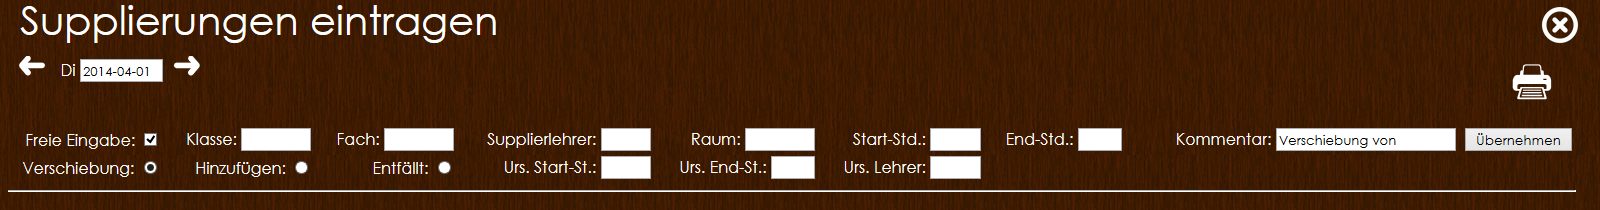
\includegraphics[keepaspectratio=true, width=17cm]{images/screenshots/substitudes_move.png}
\caption{Eingabemaske Verschiebung}
\label{fig:instr_substitudes_subMove}
\end{figure}
\subsubsection{Hinzufügen}\label{sec:instr_admin_sub_add}
Diese Eingabemethode dient dazu, zusätzliche Schulstunden an einem Tag einzufügen. Der neue Eintrag überschreibt den ursprünglichen Stundenplan der Klasse für diesen Tag.\\
Die Eingabemaske entspricht jener der Normalen Eingabe und enthält zusätzlich die Radio-Buttons (siehe \autoref{fig:instr_substitudes_subAdd}).
\begin{table}[H]
\centering
\begin{tabular}{p{3 cm}p{6 cm}p{5 cm}}
   \toprule
   \textbf{Eingabefeld} & \textbf{Typ} & \textbf{Wertebereich} \\
   \midrule
          \textbf{Freie Eingabe} & Checkbox \newline gesetzt & \\
          \hline
          \textbf{Klasse} & Listenfeld - Pflichtfeld & Abteilungs-abhängig \\
          \hline
          \textbf{Fach} & Listenfeld - optional & \\
          \hline
          \textbf{Supplierlehrer} & Listenfeld - Pflichtfeld & \\
          \hline
          Raum & Listenfeld - optional & \\
          \hline
          \textbf{Start-Std.} & Erste Schulstunde  -Pflichtfeld & 1-16 \\
		  \hline
          \textbf{End-Std.} & Letzte Schulstunde -Pflichtfeld & 1-16 \newline größer oder gleich Start-Std.\\
          \hline
          Kommentar & Textfeld - optional & \\
          \hline
          \textbf{Radio-Button} & Verschiebung - nicht gesetzt\newline 
          \textbf{Hinzufügen} - gesetzt \newline Entfällt - nicht gesetzt & \\
   \bottomrule
\end{tabular}
\caption{Eingabefelder Hinzufügen}
\end{table}
Mit der Schaltfläche Übernehmen wird eine Plausibilitätsüberprüfung durchgeführt und bei fehlerfreier Eingabe übernommen. Bei einer Fehleingabe wird der Fehler angezeigt und muss korrigiert werden. Nach der korrekten Übernahme wird die Checkbox Löschen in der erfassten Eingabezeile eingeblendet.
\begin{figure}[H]
\centering
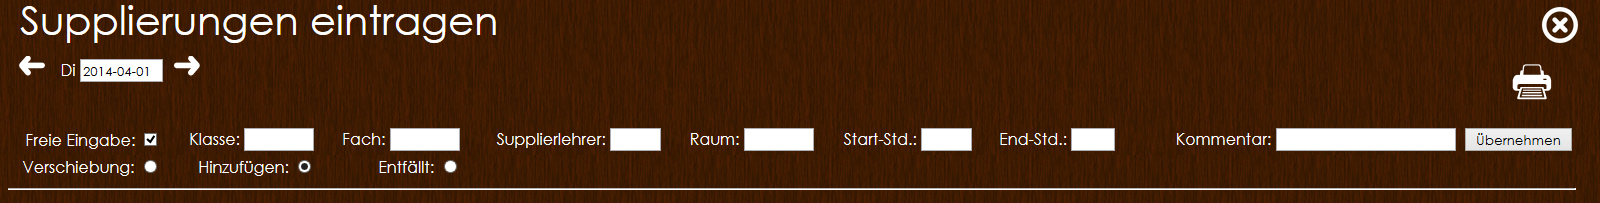
\includegraphics[keepaspectratio=true, width=17cm]{images/screenshots/substitudes_add.png}
\caption{Eingabemaske Hinzufügen}
\label{fig:instr_substitudes_subAdd}
\end{figure}
\subsubsection{Entfallen}\label{sec:instr_admin_sub_remove}
Entfällt eine Schulstunden ersatzlos, ist der Radio-Button Entfällt zu setzen. Die angegebene Stunde wird im Stundenplan der Schüler und Lehrer gelöscht.\\
Die Eingabemaske wird auf die unbedingt notwendigen Felder reduziert (siehe \autoref{fig:instr_substitudes_subRemove}).
\begin{table}[H]
\centering
\begin{tabular}{p{3 cm}p{6 cm}p{5 cm}}
   \toprule
   \textbf{Eingabefeld} & \textbf{Typ} & \textbf{Wertebereich} \\
   \midrule
          \textbf{Freie Eingabe} & Checkbox \newline gesetzt & \\
          \hline
          \textbf{Klasse} & Listenfeld - Pflichtfeld & Abteilungs-abhängig \\
          \hline
          Kommentar & Wird automatisch mit \enquote{entfällt} befüllt & \\
          \hline
          \textbf{Radio-Button} & Verschiebung - nicht gesetzt\newline Hinzufügen - nicht gesetzt \newline \textbf{Entfällt} - gesetzt & \\
          \hline
          \textbf{Urs. Start-Std.} & Erste ursprüngliche Schulstunde die Entfällt  -Pflichtfeld & 1-16 \\
          \hline
          \textbf{Urs. End-Std.} & Letzte ursprüngliche Schulstunde die Entfällt  -Pflichtfeld & 1-16 \newline größer oder gleich Urs. Start-Std.\\
          \hline
          \textbf{Urs. Lehrer} & Listenfeld - Pflichtfeld \newline ursprünglicher Lehrer der entfallenen Schulstunde\\
   \bottomrule
\end{tabular}
\caption{Eingabefelder Entfällt}
\end{table}
Mit der Schaltfläche Übernehmen wird eine Plausibilitätsüberprüfung durchgeführt und bei fehlerfreier Eingabe übernommen. Bei einer Fehleingabe wird der Fehler angezeigt und muss korrigiert werden. Nach der korrekten Übernahme wird die Checkbox Löschen in der erfassten Eingabezeile eingeblendet.
\begin{figure}[H]
\centering
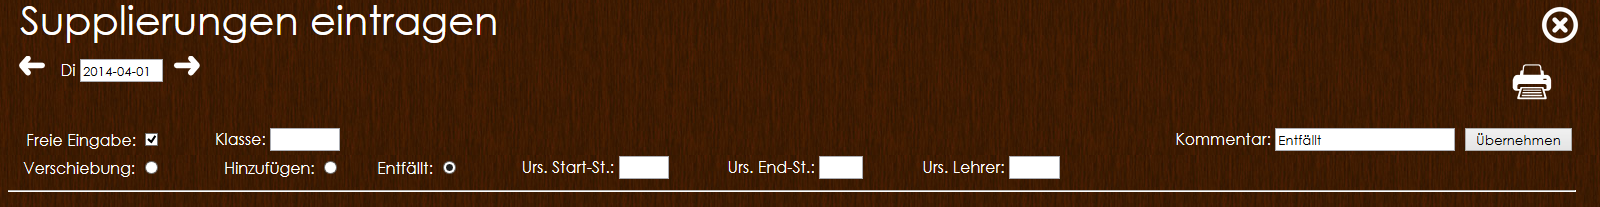
\includegraphics[keepaspectratio=true, width=17cm]{images/screenshots/substitudes_remove.png}
\caption{Eingabemaske Entfallen}
\label{fig:instr_substitudes_subRemove}
\end{figure}
\subsection{Fehler}
Wird in einem Eingabefeld ein Wert eingegeben, der nicht in der angezeigten Liste vorkommt oder nicht im Wertebereich liegt, wird ein Fehler zurückgegeben. In einem Pop-Up wird der Name des fehlerhaften Eingabefeldes angezeigt. Das Pop-Up ist mit der Schaltfläche Ok zu bestätigen. Anschließend muss die Eingabe erneut erfolgen.\\
Eine weitere Fehlerquelle kann darin liegen, dass bei der Normalen Eingabe (siehe \autoref{sec:instr_admin_sub_noFree}) zur Erfassung einer Supplierung ein ursprünglicher Lehrer gewählt wird, der nicht als fehlend erfasst wurde oder wenn die ursprüngliche Stunde nicht gefunden wird. Diese Fehler werden unter der Seitenüberschrift angezeigt und die Trennlinie unter der Eingabezeile wird rot (siehe \autoref{fig:instr_substitudes_fail}).
\begin{figure}[H]
\centering
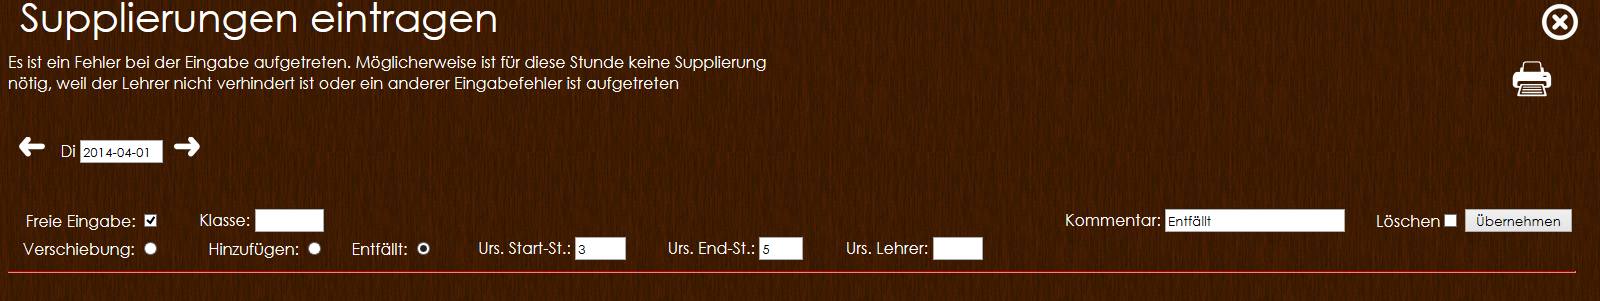
\includegraphics[keepaspectratio=true, width=17cm]{images/screenshots/substitudes_fail.png}
\caption{Fehleingabe}
\label{fig:instr_substitudes_fail}
\end{figure}
\subsection{Einträge ändern}
Bestehende Einträge können durch überschreiben geändert werden. Die Änderungen werden nach dem Drücken auf die Schaltfläche Übernehmen der Eingabezeile übernommen, sofern kein Fehler auftritt. Bei einer Fehlermeldung ist die Eingabe entsprechend zu korrigieren.
\subsection{Löschen}
Das Löschen eines Eintrages erfolgt über die Checkbox Löschen der entsprechenden Eingabezeile. Diese muss gesetzt und dann mit Übernehmen bestätigt werden. Es erfolgt keine weitere Sicherheitsabfrage und ist der Eintrag unwiderruflich gelöscht

\newpage
\section{Administrative Eingaben}

Alle im folgendem beschriebenen Eingaben (siehe \autoref{fig:instr_other_menu}) sind ausschließlich für den Super-User sichtbar. Der Einstieg erfolgt über den Punkt Administrator im Menü „Data-Input“.
\begin{figure}[H]
\centering
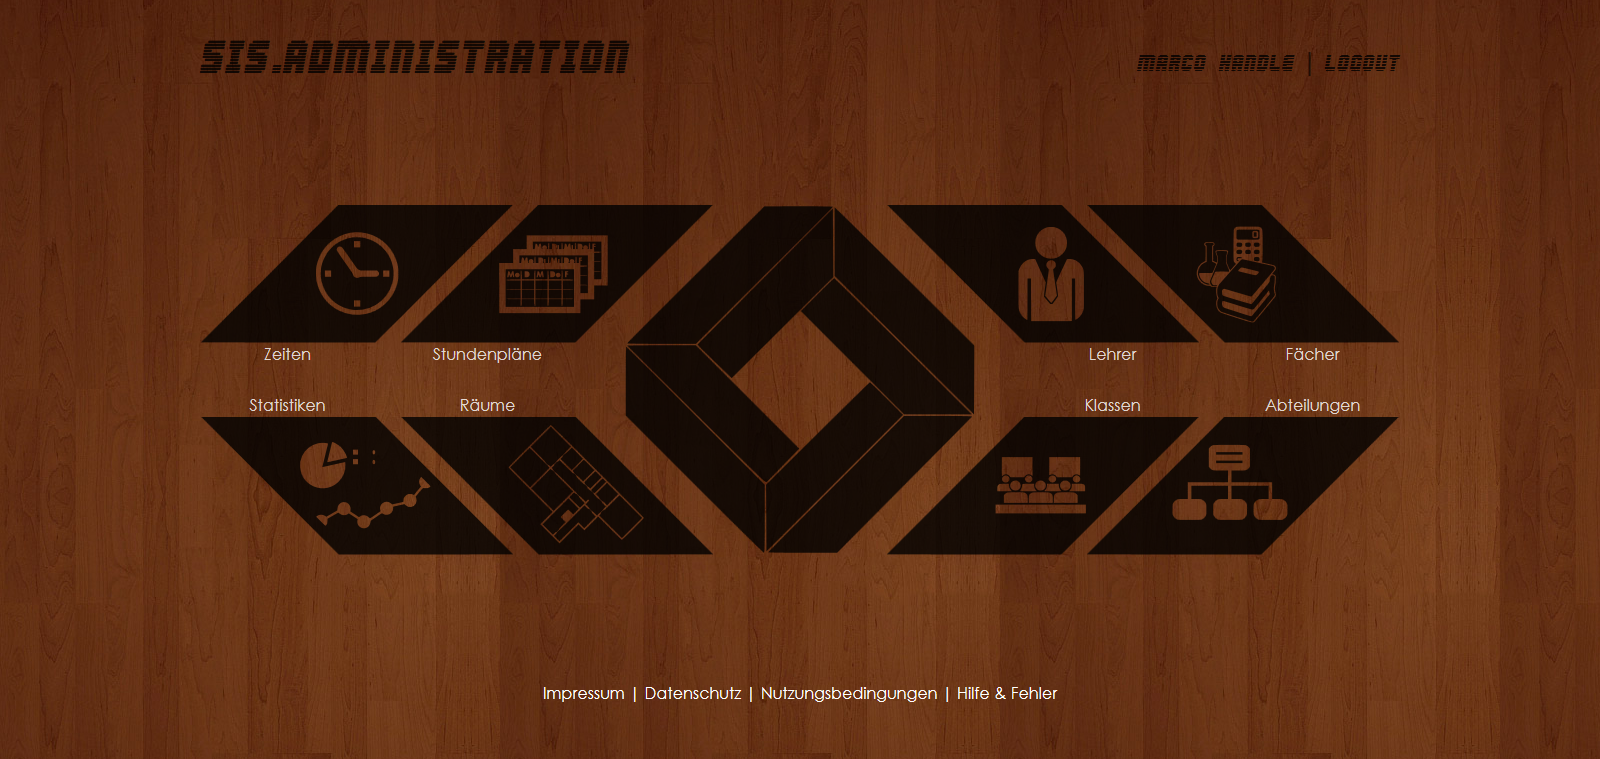
\includegraphics[keepaspectratio=true, width=17cm]{images/screenshots/admin_menu.png}
\caption{Administrationsmenü}
\label{fig:instr_other_menu}
\end{figure}
\subsection{Stunden}\label{sec:instr_other_hours}
Standardmäßig sind 16 Schulstunden mit der jeweiligen Start- und Endzeit für jeden Wochentag (Montag bis Freitag) angelegt (siehe \autoref{fig:instr_other_hours}). Über die Schaltfläche am linken bzw. rechten Seitenrand kann zwischen den Wochentagen gewechselt werden. Die Anzeige der Stunden wird entsprechend angepasst.\\
Die Änderungen können nun in den Eingabezeilen vorgenommen oder auch eine weitere Stunde angefügt werden. Alle Eingabefelder sind Pflichtfelder. Die Übernahme erfolgt mit der Schaltfläche Übernehmen in der jeweiligen Eingabezeile.\\
Aus Gründen der Datenkonsistenz der Stunden- und Supplierpläne ist das Löschen von Stunden nicht möglich.
\begin{figure}[H]
\centering
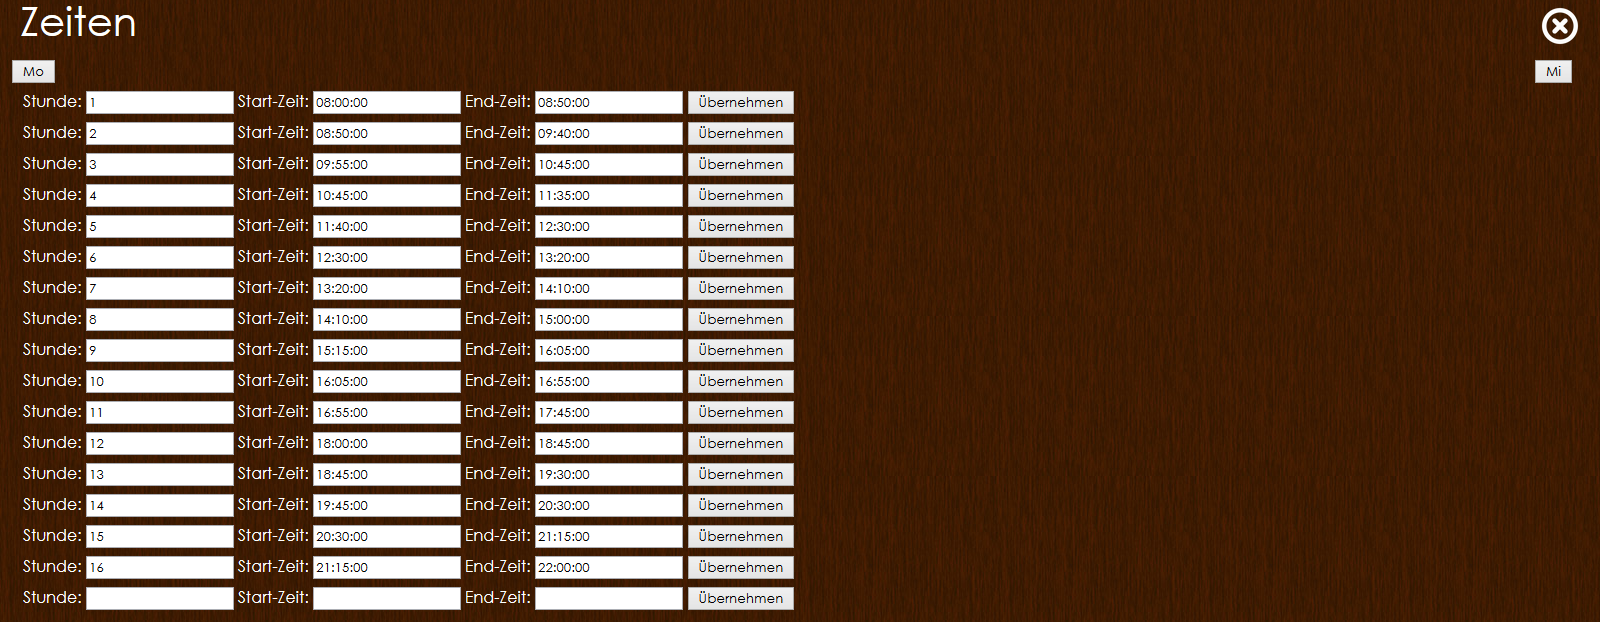
\includegraphics[keepaspectratio=true, width=17cm]{images/screenshots/hours_input.png}
\caption{Stunden bearbeiten}
\label{fig:instr_other_hours}
\end{figure}
\subsection{Stundenpläne}
Für die Erfassung eines Stundenplanes muss zuerst die Klasse (Listenfeld) und der Wochentag (Listenfeld) ausgewählt werden. Die Auswahl des Wochentages ist mit der Schaltfläche OK zu bestätigen (siehe \autoref{fig:instr_other_timetables_menu}). Ist bereits ein Stundenplan für den Tag vorhanden, wird dieser geladen (siehe \autoref{fig:instr_other_timetables_layout}). Über die Schaltfläche am linken bzw. rechten Seitenrand kann zwischen den Wochentagen gewechselt werden. Die Anzeige der Stunden wird entsprechend angepasst (siehe \autoref{fig:instr_other_timetables_day}).
Links oben werden die Klasse und der Wochentag angezeigt. Mit einem Klick auf die Klasse kehrt man ins Menü für die Auswahl der Klasse zurück (siehe \autoref{fig:instr_other_timetables_infos}).
\begin{figure}[H]
\centering

\includegraphics[keepaspectratio=true, width=17cm]{images/screenshots/timetables_input_menu.png}
\caption{Stundenplan auswählen}
\label{fig:instr_other_timetables_menu}
\end{figure}
\begin{figure}[H]
\centering

\includegraphics[keepaspectratio=true, width=6cm]{images/screenshots/timetables_input_infos.png}
\caption{Klasse und Tag}
\label{fig:instr_other_timetables_infos}
\end{figure}
\begin{figure}[H]
\centering

\includegraphics[keepaspectratio=true, width=17cm]{images/screenshots/timetables_input_day.png}
\caption{Tagauswahl}
\label{fig:instr_other_timetables_day}
\end{figure}
\begin{figure}[H]
\centering
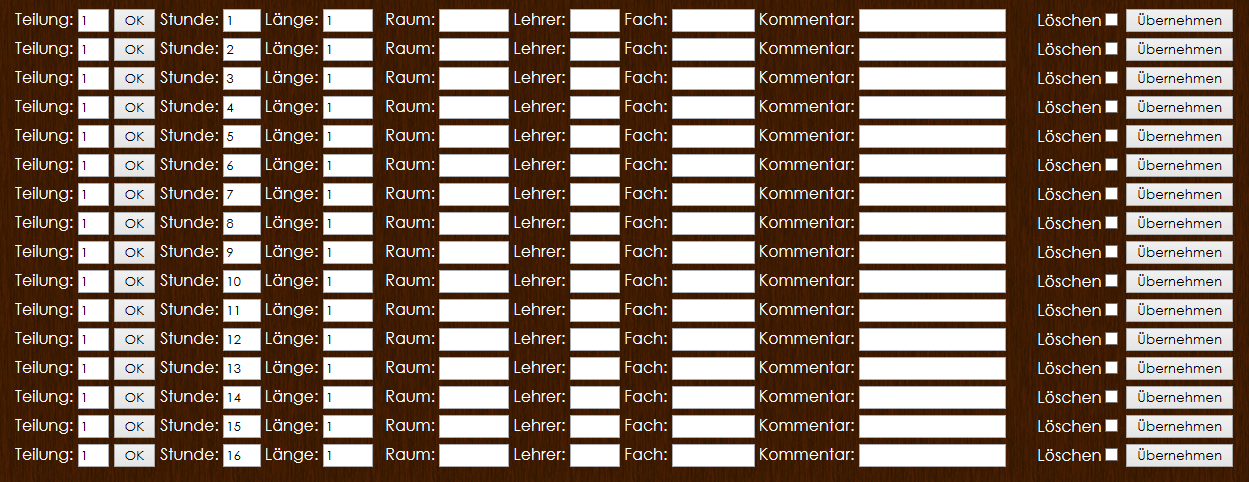
\includegraphics[keepaspectratio=true, width=17cm]{images/screenshots/timetables_input_layout.png}
\caption{Eingabemaske}
\label{fig:instr_other_timetables_layout}
\end{figure}
\subsubsection{Einstündiges Fach} \label{sec:instr_other_timetables_single}
Über die Standardeinstellung können Einzelstunden erfasst werden. In der entsprechenden Schulstunde sind der Lehrer und das Fach anzugeben.
\begin{table}[H]
\centering
\begin{tabular}{p{3 cm}p{10 cm}}
   \toprule
   \textbf{Eingabefeld} & \textbf{Typ} \\
   \midrule
          Teilung & \textbf{1} \newline nicht ändern \\
          \hline
          OK & Schaltfläche \\
          \hline
          Stunde & Schulstunde \newline Kann nicht geändert werden\\
          \hline
          Länge & \textbf{1} \newline Nicht ändern \\
          \hline
          Raum & Listenfeld - optional \\
          \hline
          \textbf{Lehrer} & Listenfeld - Pflichtfeld \\
		  \hline
          \textbf{Fach} & Listenfeld - Pflichtfeld.\\
          \hline
          Kommentar & Textfeld - optional \\
          \hline
          Löschen & Checkbox - \textbf{nicht gesetzt}\\
   \bottomrule
\end{tabular}
\caption{Eingabefelder Stundenplan}
\end{table}
Die Änderungen bzw. Ergänzungen sind mit der Schaltfläche Übernehmen in der jeweiligen Eingabezeile zu übernehmen (siehe \autoref{fig:instr_other_timetables_singleHour}).
\begin{figure}[H]
\centering

\includegraphics[keepaspectratio=true, width=17cm]{images/screenshots/timetables_input_singleHour.png}
\caption{Beispiel Einzelstunde}
\label{fig:instr_other_timetables_singleHour}
\end{figure}
\subsubsection{Mehrstündiges Fach}
Die Eingabe erfolgt analog zu jener im \autoref{sec:instr_other_timetables_single} beschriebenen. Es ist aber im Eingabefeld Länge die Anzahl der zusammenhängenden Schulstunden anzugeben. Wird nun in ein anderes Eingabefeld gewechselt, werden die nachfolgenden Eingabezeilen ausgeblendet, welche durch das mehrstündige Fach abgedeckt werden (siehe \autoref{fig:instr_other_timetables_multiHour}).\\
Wird zum Beispiel in der ersten Stunde ein Fach mit der Länge von 3 Stunden eingetragen, werden die Eingabezeilen der zweiten und dritte Stunde ausgeblendet.\\
Eingaben und Änderungen müssen jeweils durch das Drücken auf die Schaltfläche Übernehmen übernommen werden.
\begin{figure}[H]
\centering
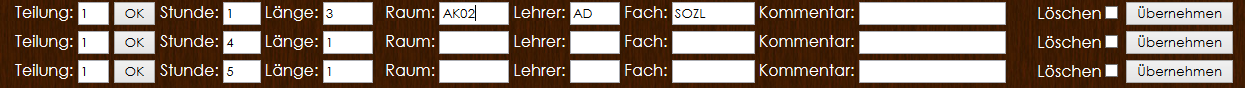
\includegraphics[keepaspectratio=true, width=17cm]{images/screenshots/timetables_input_multiHour.png}
\caption{Beispiel Mehrstündiger Unterricht}
\label{fig:instr_other_timetables_multiHour}
\end{figure}
\subsubsection{Teilung von Klassen}
Wird eine Klasse im Unterricht geteilt, ist dies über das Eingabefeld Teilung zu erfassen. Es ist zu beachten, dass die geteilten Fächer gleich lang sein müssen. Sind die geteilten Fächer ungleich lang, so ist der Rest der längeren Teilung als Einzelstunde zu erfassen. Eine Klasse kann maximal in 7 Teile geteilt werden.\\
Um eine Teilung erfassen zu können, ist im Eingabefeld Teilung die Anzahl der Teilungen einzugeben und mit der Schaltfläche OK zu bestätigen. Anschließend erscheinen weitere Eingabezeilen (siehe \autoref{fig:instr_other_timetables_divide7}).\\
Die Eingabe erfolgt sinngemäß wie die Erfassung eines mehrstündigen Fachs. Jede einzelne Eingabezeile der Teilung ist mit der Schaltfläche Übernehmen zu bestätigen.
\begin{figure}[H]
\centering
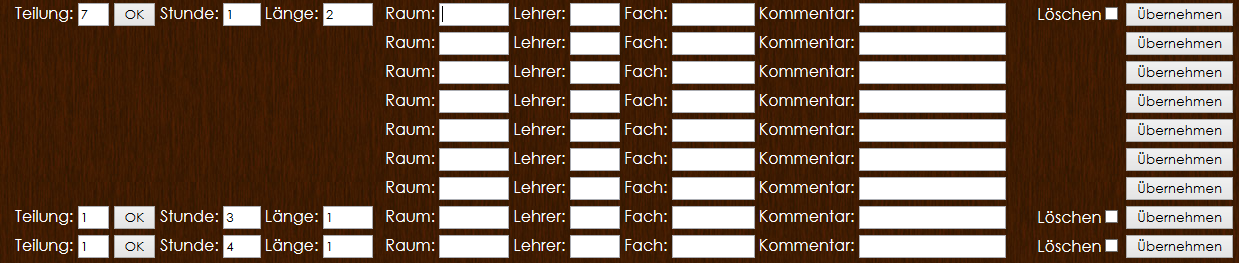
\includegraphics[keepaspectratio=true, width=17cm]{images/screenshots/timetables_input_divide7.png}
\caption{Beispiel Teilungen}
\label{fig:instr_other_timetables_divide7}
\end{figure}
Jede eigene Zeile muss mit Übernehmen bestätigt werden. Gelöscht kann jedoch nur ein ganzer Block werden. Dies muss mit einem Hacken bei Löschen und anschließendem Klicken auf Übernehmen erfolgen.
\subsubsection{Löschen von Unterrichtsstunden}
Das Löschen von Einträgen kann einzeln über die Checkbox Löschen vorgenommen werden. Der Stundenplan eines Tages kann über die Schaltfläche \enquote{Stundenplan löschen} \textbf{unwiderruflich} gelöscht werden (siehe \autoref{fig:instr_other_timetables_delete}).
\begin{figure}[H]
\centering

\includegraphics[keepaspectratio=true, width=5cm]{images/screenshots/timetables_input_delete.png}
\caption{Löschen}
\label{fig:instr_other_timetables_delete}
\end{figure}
\subsection{Lehrer}
Dieser Punkt ist dazu da, dass man Lehrer bearbeiten und hinzufügen kann. Auch hier ist es nicht möglich Lehrer zu löschen, da es wie bei Stunden zu großen Problemen kommen kann. (siehe \autoref{sec:instr_other_hidden})\\
Im Feld Name muss der vollständige Name des Lehrers eingegeben werden, im Feld Kürzel wird das Lehrer-Kürzel eingetragen, im Feld Kurzname muss ein verkürzter Name eingegeben werden, dieser wird zum Beispiel bei den Supplierungen am Display angezeigt. Im Feld Stammabteilung kann eine Abteilung eingegeben werden, dies ist jedoch optional, da nicht jeder Lehrer eine Stammabteilung hat. Wie schon erwähnt ist der Hacken für unsichtbar zum stilllegen eines Lehrers gut. (Eingabemaske siehe \autoref{fig:instr_other_teacher}) Sollen vorhandene Daten geändert werden, so kann man den vorhandenen Lehrer abändern und mit Übernehmen speichern.
\begin{figure}[H]
\centering

\includegraphics[keepaspectratio=true, width=17cm]{images/screenshots/teachers_input.png}
\caption{Eingabemaske Lehrer}
\label{fig:instr_other_teacher}
\end{figure}
\subsection{Fächer}
Über diese Eingabemaske werden Lehrereinträge bearbeitet und hinzugefügt (siehe \autoref{fig:instr_other_subjects}). Aus Gründen der Datenkonsistenz der Stunden- und Supplierpläne ist das Löschen von Lehrern nicht möglich.
\begin{table}[H]
\centering
\begin{tabular}{p{3 cm}p{10 cm}}
   \toprule
   \textbf{Eingabefeld} & \textbf{Typ} \\
   \midrule
          \textbf{Name} & Textfeld - Pflichtfeld \newline vollständiger Name \\
          \hline
          \textbf{Kürzel} & Textfeld - Pflichtfeld \newline Lehrer-Kürzel \\
          \hline
          \textbf{Kurzname} & Textfeld - Pflichtfeld \newline Kurzname für die Anzeige am Display \\
          \hline
          Stammabteilung & Textfeld - optional \\
          \hline
          Unsichtbar & Checkbox \\
   \bottomrule
\end{tabular}
\caption{Eingabefelder Fächer}
\end{table}
Wird die Checkbox Unsichtbar bei einem Lehrer gesetzt, wird dieser in den Listenfelder nicht mehr angezeigt. (siehe \autoref{sec:instr_other_hidden})\\
Änderungen und Ergänzungen sind über die Schaltfläche Übernehmen in den Eingabezeilen zu bestätigen.
\begin{figure}[H]
\centering
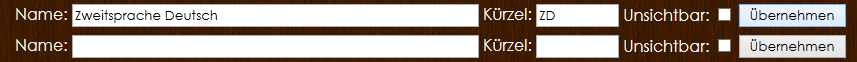
\includegraphics[keepaspectratio=true, width=17cm]{images/screenshots/subjects_input.png}
\caption{Eingabemaske Fächer}
\label{fig:instr_other_subjects}
\end{figure}
\subsection{Statistiken}
Um die Akzeptanz der Anwendung beurteilen zu können, wurde ein Statistikmodul implementiert, obwohl dies im vorgegebenen Pflichtenheft nicht vorgesehen ist. Es werden deshalb unter anderem anonymisiert die Zugriffe auf die verschiedenen Seiten, von welchen Endgeräten die Zugriffe erfolgen, welche Schulstufen, etc. registriert und in Grafiken ausgewertet.
\begin{figure}[H]
\centering

\includegraphics[keepaspectratio=true, width=17cm]{images/screenshots/statistics_header.png}
\caption{Statistiken Reload}
\label{fig:instr_other_statistics_header}
\end{figure}
\subsubsection{Browser PC}
In dieser Statistik sind die Browser der Geräte dargestellt, welche die PC Seiten aufrufen. (siehe \autoref{fig:instr_other_statistics_browser_PC})
\begin{figure}[H]
\centering
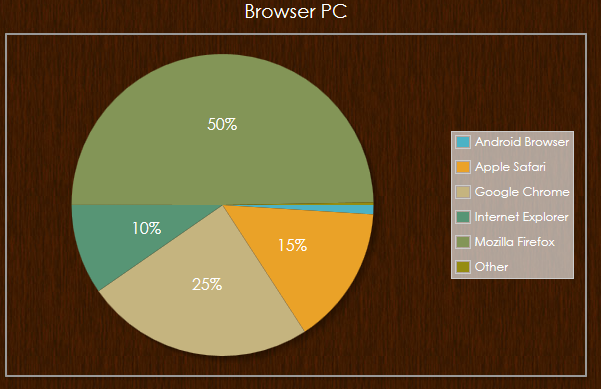
\includegraphics[keepaspectratio=true, width=8cm]{images/screenshots/statistics_browser_PC.png}
\caption{Browser PC}
\label{fig:instr_other_statistics_browser_PC}
\end{figure}
\subsubsection{Geräte PC}
In dieser Statistik sind die Geräte bzw. Betriebssysteme der Geräte dargestellt, welche die PC Seiten aufrufen. (siehe \autoref{fig:instr_other_statistics_os_PC})
\begin{figure}[H]
\centering
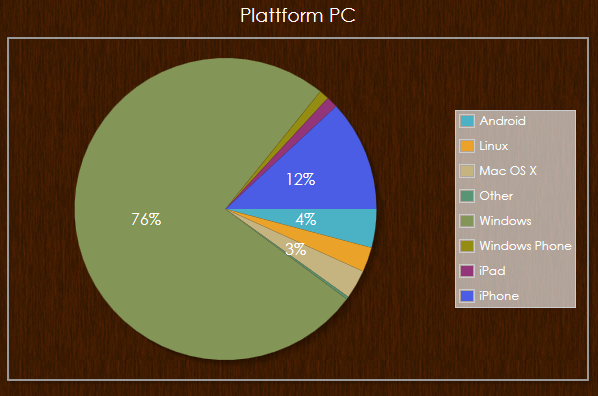
\includegraphics[keepaspectratio=true, width=8cm]{images/screenshots/statistics_os_PC.png}
\caption{Geräte PC}
\label{fig:instr_other_statistics_os_PC}
\end{figure}
\subsubsection{Browser Mobil}
In dieser Statistik sind die Browser der Geräte dargestellt, welche die App aufrufen. (siehe \autoref{fig:instr_other_statistics_browser_Mob})
\begin{figure}[H]
\centering
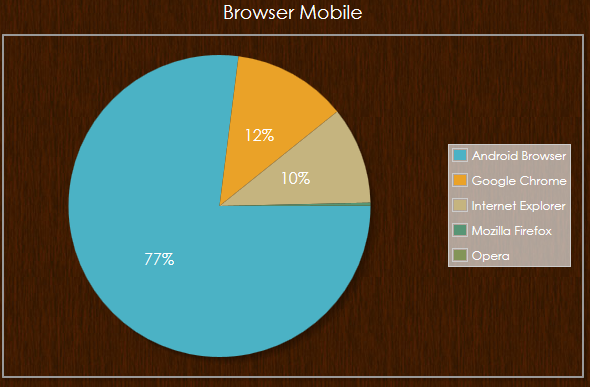
\includegraphics[keepaspectratio=true, width=8cm]{images/screenshots/statistics_browser_Mob.png}
\caption{Browser Mobil}
\label{fig:instr_other_statistics_browser_Mob}
\end{figure}
\subsubsection{Geräte Mobil}
In dieser Statistik sind die Geräte bzw. Betriebssysteme der Geräte dargestellt, welche die App Seiten aufrufen. (siehe \autoref{fig:instr_other_statistics_os_Mob})
\begin{figure}[H]
\centering
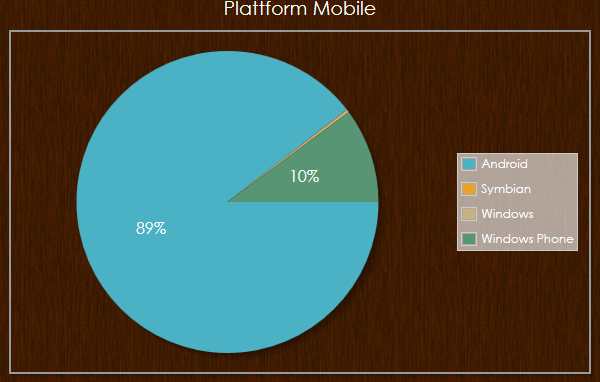
\includegraphics[keepaspectratio=true, width=8cm]{images/screenshots/statistics_os_Mob.png}
\caption{Browser PC}
\label{fig:instr_other_statistics_os_Mob}
\end{figure}
\subsubsection{Nutzer}
In dieser Statistik sind die Nutzer nach den Schulstufen und nach den Lehrern aufgeteilt. Hier kann herausgelesen werden welcher Jahrgang den Service am häufigsten nutzt. (siehe \autoref{fig:instr_other_statistics_user})
\begin{figure}[H]
\centering
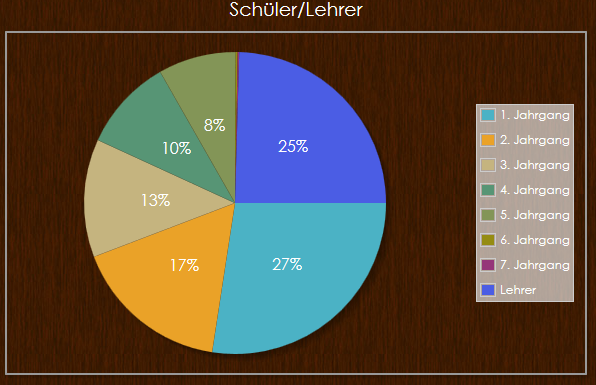
\includegraphics[keepaspectratio=true, width=8cm]{images/screenshots/statistics_user.png}
\caption{Nutzer}
\label{fig:instr_other_statistics_user}
\end{figure}
\subsubsection{Abteilungen}
In dieser Statistik werden die Nutzer nach ihrer Abteilung aufgeteilt, dabei werden nur die Schüler gezählt. Hier kann herausgelesen werden welche Abteilung den Service am häufigsten nutzt. (siehe \autoref{fig:instr_other_statistics_sections})
\begin{figure}[H]
\centering
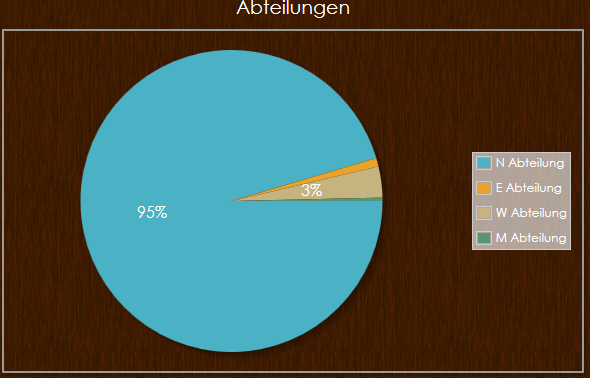
\includegraphics[keepaspectratio=true, width=8cm]{images/screenshots/statistics_sections.png}
\caption{Abteilungen}
\label{fig:instr_other_statistics_sections}
\end{figure}
\subsubsection{Supplierunen}
In dieser Statistik wird dargestellt welche Seite die User am häufigsten benützen, um die Supplierungen anzusehen. Dabei wird der Supplierplan im Web, Supplierplan in der App , der modifizierte Stundenplan in der App und der modifizierte Stundenplan im Web analysiert. (siehe \autoref{fig:instr_other_statistics_substitudes})
\begin{figure}[H]
\centering
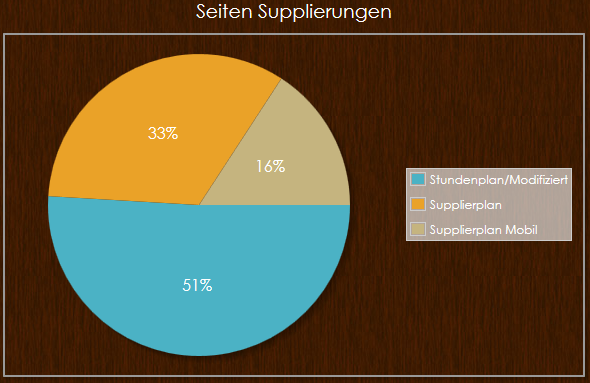
\includegraphics[keepaspectratio=true, width=8cm]{images/screenshots/statistics_substitudes.png}
\caption{Supplierungen}
\label{fig:instr_other_statistics_substitudes}
\end{figure}
\subsubsection{App/Web}
In dieser Statistik wird die App und die Webseite gegenübergestellt und man kann auslesen welcher Dienst öfters genutzt wird. (siehe \autoref{fig:instr_other_statistics_app_web})
\begin{figure}[H]
\centering
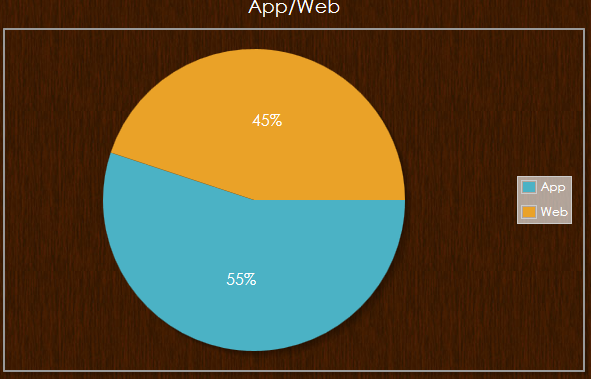
\includegraphics[keepaspectratio=true, width=8cm]{images/screenshots/statistics_app_web.png}
\caption{App/Web}
\label{fig:instr_other_statistics_app_web}
\end{figure}
\subsubsection{Seiten Web}
In dieser Statistik wird dargestellt welche Seiten die User auf der Webseite am häufigsten besuchen. (siehe \autoref{fig:instr_other_statistics_sites_web})
\begin{figure}[H]
\centering
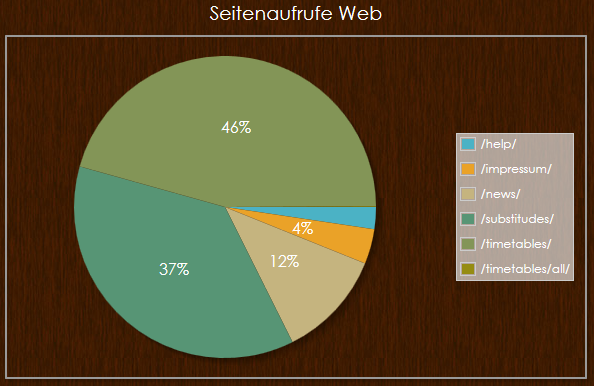
\includegraphics[keepaspectratio=true, width=8cm]{images/screenshots/statistics_sites_web.png}
\caption{Seiten Web}
\label{fig:instr_other_statistics_sites_web}
\end{figure}
\subsubsection{Seiten App}
In dieser Statistik wird dargestellt welche Seiten die User in der App am häufigsten besuchen. (siehe \autoref{fig:instr_other_statistics_sites_app})
\begin{figure}[H]
\centering
\includegraphics[keepaspectratio=true, width=8cm]{images/screenshots/statistics_sites_app.png}
\caption{Seiten App}
\label{fig:instr_other_statistics_sites_app}
\end{figure}
\subsubsection{Seitenaufrufe Stunden}
In dieser Statistik wird dargestellt, wie viele Seitenaufrufe im Durchschnitt in welcher Stunde am Tag auftreten. (siehe \autoref{fig:instr_other_statistics_view_day})
\begin{figure}[H]
\centering
\includegraphics[keepaspectratio=true, width=17cm]{images/screenshots/statistics_views_hour.png}
\caption{Seitenaufrufe Stunden}
\label{fig:instr_other_statistics_view_day}
\end{figure}
\subsubsection{Seitenaufrufe täglich}
In dieser Statistik wird dargestellt, wie viele Seitenaufrufe jeden Tag verursacht werden. (siehe \autoref{fig:instr_other_statistics_views_day}) Hier kann auch, um bei vielen Tagen sich einen Überblick zu beschaffen, hineingezoomt werden. Dies macht man in dem man mit der linken Maustaste ein gewünschtes Fenster aufzieht. Heraus zoomen kann mit einem doppelten rechts Klick gemacht werden. (siehe \autoref{fig:instr_other_statistics_views_day_zoom})
\begin{figure}[H]
\centering
\includegraphics[keepaspectratio=true, width=17cm]{images/screenshots/statistics_views_day.png}
\caption{Seitenaufrufe täglich}
\label{fig:instr_other_statistics_views_day}
\end{figure}
\begin{figure}[H]
\centering
\includegraphics[keepaspectratio=true, width=17cm]{images/screenshots/statistics_views_day_zoom.png}
\caption{Seitenaufrufe täglich zoomen}
\label{fig:instr_other_statistics_views_day_zoom}
\end{figure}
\subsection{Räume}
Über diese Eingabemaske werden Räume bearbeitet und hinzugefügt (siehe \autoref{fig:instr_other_room_input}). Aus Gründen der Datenkonsistenz der Stunden- und Supplierpläne ist das Löschen von Räumen nicht möglich.
\begin{table}[H]
\centering
\begin{tabular}{p{3 cm}p{10 cm}}
   \toprule
   \textbf{Eingabefeld} & \textbf{Typ} \\
   \midrule
          \textbf{Name} & Textfeld - Pflichtfeld \newline Name des Raumes \\
          \hline
          Zuständiger Lehrer & Listenfeld - optional \newline Verantwortlicher Lehrer für den Raum\\
   \bottomrule
\end{tabular}
\caption{Eingabefelder Räume}
\end{table}
Änderungen und Ergänzungen sind über die Schaltfläche Übernehmen in den Eingabezeilen zu bestätigen.
\begin{figure}[H]
\centering
\includegraphics[keepaspectratio=true, width=10cm]{images/screenshots/rooms_input.png}
\caption{Eingabemaske Räume}
\label{fig:instr_other_room_input}
\end{figure}
\subsection{Klassen}
Über diese Eingabemaske werden Klassen bearbeitet und hinzugefügt (siehe \autoref{fig:instr_other_classes_input}). Aus Gründen der Datenkonsistenz der Stunden- und Supplierpläne ist das Löschen von Klassen nicht möglich. Jedoch können Klassen als unsichtbar gekennzeichnet werden (siehe \autoref{sec:instr_other_hidden}).
\begin{table}[H]
\centering
\begin{tabular}{p{3 cm}p{10 cm}}
   \toprule
   \textbf{Eingabefeld} & \textbf{Typ} \\
   \midrule
          \textbf{Name} & Textfeld - Pflichtfeld \newline Name der Klasse \\
          \hline
          \textbf{Abteilung} & Listenfeld - Pflichtfeld \\
          \hline
          Klassenvorstand & Listenfeld - optional \\
          \hline
          Stammklasse & Textfeld - optional \newline Zugeordneter Klassenraum \\
          \hline
          Unsichtbar & Checkbox \\
   \bottomrule
\end{tabular}
\caption{Eingabe Klassen}
\end{table}
Wanderklassen kann der Raum WK als Scheinklassenraum zugewiesen werden. Wird die Checkbox Unsichtbar bei einer Klasse gesetzt, wird diese in den Listenfelder nicht mehr angezeigt.\\
Änderungen und Ergänzungen sind über die Schaltfläche Übernehmen in den Eingabezeilen zu bestätigen.
\begin{figure}[H]
\centering
\includegraphics[keepaspectratio=true, width=17cm]{images/screenshots/classes_input.png}
\caption{Eingabemaske Klassen}
\label{fig:instr_other_classes_input}
\end{figure}
\subsection{Abteilungen}
Über diese Eingabemaske werden Abteilungen bearbeitet und hinzugefügt (siehe \autoref{fig:instr_other_sections_input}). Aus Gründen der Datenkonsistenz der Stunden- und Supplierpläne ist das Löschen von Abteilungen nicht möglich.
\begin{table}[H]
\centering
\begin{tabular}{p{3 cm}p{10 cm}}
   \toprule
   \textbf{Eingabefeld} & \textbf{Typ} \\
   \midrule
          \textbf{Name} & Textfeld - Pflichtfeld \newline Vollständiger Bezeichnung der Abteilung \\
          \hline
          \textbf{Kürzel} & Listenfeld - Pflichtfeld \\
          \hline
          \textbf{Abteilungsleiter} & Listenfeld - Pflichtfeld \\
   \bottomrule
\end{tabular}
\caption{Eingabe Abteilungen}
\end{table}
\begin{figure}[H]
\centering
\includegraphics[keepaspectratio=true, width=17cm]{images/screenshots/sections_input.png}
\caption{Eingabemaske Abteilungen}
\label{fig:instr_other_sections_input}
\end{figure}
\subsection{Unsichtbar}\label{sec:instr_other_hidden}
Aus Sicherheitsgründen und Gründen der Datenkonsistenz dürfen manche Daten nicht gelöscht werden. Das Löschen ist nur dort möglich, wo explizit eine Checkbox Löschen vorhanden ist.\\
Um dennoch unnötige Einträge in den Listenfeldern zu vermeiden, können über die Checkbox Unsichtbar Einträge deaktiviert werden. Über die gleiche Funktion können diese Einträge dann wenn notwendig wieder aktiviert werden.
\subsection{DropDown-Menüs}
In zahlreichen Eingabefeldern sind Listen der zulässigen Eingaben hinterlegt, welche bei Beginn der Eingabe angezeigt werden. In Abhängigkeit der eingegebenen Zeichen wird die angezeigte Liste eingeschränkt. Ist die angezeigte Liste leer, so wurde kein übereinstimmender Eintrag gefunden und liegt wahrscheinlich eine Fehleingabe vor.

\chapter{Begleitendes FTKL-Projekt}
\label{sec:report}
\section{Aufgabenstellung}
Es sollte eine Möglichkeit geschaffen werden, die Monitore, welche an vielen Stellen in der Schule positioniert sind, zentral stromfrei zu schalten.

\section{Hardware}
\subsection{Überlegungen}
Für die Umsetzung wurden handelsübliche Funksteckdosen verwendet, da diese relativ günstig in den meisten Geschäften zu haben sind. Diese erfüllen jedoch Standardmäßig einen anderen Zweck, diese werden über eine Fernbedienung ein bzw. aus geschaltet. Da es uns nicht möglich ist, Steckdosen mit dem Raspberry über Funk zu steuern, musste eine andere Möglichkeit her.\\
Uns kam die Idee, dass in diesen Steckdosen eigentlich nur ein Relais vorhanden sein muss, welches die 230V schaltet. Diese Tatsache machten wir uns zu nutze und suchten auf der Platine nach diesem Schaltpunkt und entwickelten eine passende Schaltung, welche diese Relais schaltet.\\
Um widerrechtliches steuern der Steckdosen durch gefinkelte Schüler zu verhindern und da das Funkmodul nur auf die Platine aufgelötet war, bauten wir diese Platine aus. Somit ist es nicht mehr möglich die Steckdosen mit der passenden Fernbedienung zu steuern.\\\\
Die Schaltung der Steckdose ist in keinster Weise dokumentiert, auch die auf der Schaltung vorhandenen IC's sind kaum bis gar nicht dokumentiert, weshalb es uns nicht möglich war die Funktionsweise der einzelnen Teile fest zu stellen. Durch Analysen der Leiterbahnen konnten wir uns eine grobe Übersicht über die Schaltung verschaffen. Dieser Überblick reichte jedoch nicht aus, um den Schaltpunkt des Relais zu finden. Der eigentliche Schaltpin am Relais konnte identifiziert werden, jedoch schaltet dieses Relais erst bei 48V, welche nicht angelegt werden konnte, deshalb musste eine andere Möglichkeit gefunden werden.\\ 
Die Art des Suchens war nicht sehr professionell, da wir versuchten, durch Anlegen einer Steuerspannung an bestimmte Pins der ICs, den Pin zu finden, durch welchen das Relais geschaltet wird. Nach einigen Versuchen konnte der Punkt gefunden werden, dieser war doch nicht ideal, da dessen Innenwiderstand sehr klein war, was sich dahingehend zeigte, dass der Strom, der benötigt wurde, um die Steuerspannung zu halten, sehr hoch war. Wir fanden allerdings einen besseren Punkt, welcher wesentlich weniger Strom zog. Durch das Anlegen von 5V schaltete das Relais, dies entspricht der Versorgungsspannung des Funkmoduls. Es liegt nahe, diese zu verwenden.\\
Für eine leichtere Montage wurden die Vorhandenen Kontakte des Funkmoduls verwendet. Über die Kontakte wurde die Platine versorgt, diese Funktionsweise verwendeten auch wir, weshalb wir von dem gefundenen Punkt eine Drahtbrücke zum Kontakt machten. Die 5V waren sowieso schon auf einem der Kontakte vorhanden. Um die ursprüngliche Funktion des Kontaktes ab zu schalten trennten wir durch Entfernung eines Widerstandes die Leiterbahn auf. Nun musste nur mehr die Platine in die Kontaktlöcher gesteckt werden. Die nötigen Signale sind bei den Kontakten angelegt und werden über die Verbindung auf der Platine bereitgestellt.\\
Nun musste noch eine Lösung gefunden werden, wie mit dem Raspberry diese 2 Punkte verbunden werden konnten. Dies wurde mit einer Transistorschaltung realisiert. Wenn der Raspberry an einem der GPIO-Pins digital 1 (analog 3,3V DC) anlegt, so schaltet der Transistor und verbindet somit die zwei Punkte. \\
Dies war jedoch nicht genug, da noch eine Potentialtrennung zwischen Raspberry und Steckdose  notwendig war, wie ein Test ohne Potentialtrennung zeigt. (Siehe Punkt???). Diese lösten wir mit einem Optokoppler, welcher den Raspberry von der Steckdose trennen soll. Dies erfolgte mit der Schaltung ordnungsgemäß. Jedoch packten wir die Potentialtrennung auf den Header, welcher auf den Raspberry aufgesteckt wird, dies stellte sich als fataler Fehler heraus. (siehe Punkt ????)\\
Der finale Aufbau war dann wie folgt:\\
Auf die GPIO-Pins (siehe \autoref{fig:report_hardware_gpio1}) wird eine Platine(Header) gesteckt, welche die Transistorschaltung beinhaltet. Die Transistorschaltung schaltet die 5V Versorgung über einen Vorwiderstand den Optokoppler, welcher auf einer Platine in der Steckdose liegt. Die Verbindung wurde mit einem 2 poligen Draht, welcher auf beiden Seiten eine 3,5mm Mono Stecker montiert hat. Auf der Platine in der Steckdose ist nur der Optokoppler, der das Ein- bzw. Ausschalten der Steckdose vornimmt.\\
Für die Kommunikation mit dem Raspberry wird der GPIO Pin 4 (Header Pin 7) verwendet. Die 5V Spannung und die Masse für das Schalten des Optokopplers wird der Pin 2(5V) und der Pin 6(0V) des Raspberrys verwendet. Wichtig: Hier ist anzumerken, dass die Rasperrys Revision 1 und Revision 2 verschiedene Anordnung haben. Unsere Schaltung ist für Revision 2 entwickelt, es ist also nicht zu empfehlen, die Platine auf einem Revision 1 Raspberry zu verwenden, da er Schaden nehmen könnte.
\\
\begin{figure}[H]
\centering
\includegraphics[keepaspectratio=true, width=10cm]{images/rpi/picPins.png}
\caption[GPIO-Pins]{GPIO-Pins\\ \textbf{Quelle:} http://elinux.org/Rpi\_Low-level\_peripherals}
\label{fig:report_hardware_gpio1}
% source: http://elinux.org/Rpi_Low-level_peripherals#General_Purpose_Input.2FOutput_.28GPIO.29
\end{figure}
\begin{figure}[H]
\centering
\rule{1cm}{1cm}
\includegraphics[keepaspectratio=true, width=7cm]{images/rpi/gpio.png}
% source: http://elinux.org/Rpi_Low-level_peripherals#General_Purpose_Input.2FOutput_.28GPIO.29
\caption[GPIO-Pinbelegung]{GPIO-Pinbelegung\\ \textbf{Quelle:}
\label{fig:report_hardware_gpio2} http://elinux.org/Rpi\_Low-level\_peripherals}
\end{figure}

\subsection{Probleme}
Während einer Entwicklung treten üblicherweise auch einige Probleme auf, an die nicht gedacht wurde, so auch in unserem Fall.\\
\subparagraph{Potentialtrennung}\label{sec:report_hardware_pot}
Das erste Problem, das uns auffiel, war das Problem der Potentialtrennung. Aufgrund dieses Problem kam es zu einem Kurzschluss, welcher den Raspberry zerstörte. Deshalb musste eine Potentialtrennung zwischen der Steckdose und dem Raspberry gemacht werden, damit keine hohen Spannungen auf den Raspberry übertragen werden und dadurch ein hoher Strom resultiert. Dies hat die Folge, dass der Raspberry zerstört wird. Die Lösung dieses Problem ist die Trennung mit Hilfe eines Optokopplers. Die Ausführung siehe \autoref{sec:report_hardware_th} \\
\subparagraph{Spannung auf berührbaren Teilen}\label{sec:report_hardware_spannung}
Dieses Problem hat eigentlich wieder mit der Potentialtrennung zu tun. Wir lösten die Potentialtrennung auf dem Raspberry Header, das heißt das nicht Potential getrennte Signal ist von der Steckdose über das Verbindungskabel zum Raspberry geführt worden. Dies ist jedoch nicht so dramatisch. Jedoch erzeugt die Steckdose ihr Potential für die Gleichspannungsversorgung immer fix. Das heißt die Steckdose nimmt immer, egal wie die Steckdose in der Steckdose steckt, zum Beispiel den rechten Pin der Steckdose.\\
Zu besseren Erklärung wird dies am folgendem Beispiel geschildert:\\
\begin{itemize}
	\item Nehmen wir an die Steckdose steckt mit der Position A in der Steckdose, somit hat die Schaltung als Masse den Neutralleiter, was dann, bezogen auf die Erdung, ergibt, dass die Masse gleich Erdung und die  5V gleich 5V+Erdungspotential ist. Somit ist alles in Ordnung.
	\item Nun nehmen wir an, dass die Steckdose mit Position B in der Steckdose steckt, was soviel wie eine Drehung um 180° bedeutet. Nun erzeugt die Schaltung wieder auf dem selben Prinzip die Versorgungsspannung. Nur mit dem Unterschied, dass wo zuvor der Neutralleiter war nun die Phase ist und umgekehrt. Dies hat zur Folge, dass die Schaltung die Versorgungsspannung auf Basis der Phase macht, also Masse gleich Phase gleich 230V und 5V gleich Phase+5V DC.
\end{itemize}
Somit lässt sich nun sagen, dass wir in unserem Fall, wenn die Steckdose "falsch in der Steckdose gesteckt ist", 5V+230V über das Verbindungskabel auf den Respberry Header übertragen haben und somit bei Berührung des Headers einen 230V Stromschlag bekommen haben.\\
Die Lösung dafür war, dass wir die Potentialtrennung in die Steckdose verlegten und somit nur ein Potentialfreies Signal über die Verbindungsleitung übertragen haben.

\newpage
\section{Software}
\subsection{Überlegungen}
Die GPIO-Pins lassen sich über virtuelle Dateien des Linux-Kernels ansteuern. Somit liegt hier kein Problem vor.\\
\\
Das größere Problem ist das Verteilen der Befehle auf alle Raspberry Pis. Da das Benutzerinterface sowieso in SIS integriert werden soll, liegt der Gedanke nahe, auch die Verteilung der Befehle über SIS zu managen.

\subsection{Lösung}
\subsubsection{Überlegungen}

Die Software zum regelmäßigen Anfragen am Server muss bereits beim Systemstart mitgestartet werden. Es bietet sich an, die Scripts über die Datei /etc/rc.local zu starten, da diese Datei relativ unkompliziert verwendet werden kann (\autoref{siehe lst:report_attachment_rc-local}, Seite \pageref{lst:report_attachment_rc-local}).\\

\subsubsection{Darstellung}

Damit kein Tool für den automatischen Login installiert werden muss, wird der Default-Runlevel auf % TOTO % 
gesetzt (Dies kann durch Modifikation des Schlüssels \enquote{initdefault} in der Datei /etc/inittab erreicht werden. Siehe \autoref{lst:report_attachment_inittab}, Seite \pageref{lst:report_attachment_inittab}.) und der X-Server manuell gestartet.\\
Das Starten des X-Servers wird durch das Script /usr/bin/sis-x initialisiert.

\lstinputlisting[style=custom, language=sh, caption={/usr/bin/sis-x}, label={lst:report_software_sis-x}]{sources/raspberry/sis-x.x}

Wie in \autoref{lst:report_software_sis-x} ersichtlich ist, wird überprüft, ob das Script als root gestartet wurde. Wenn dies der Fall sein sollte, dann startet das Script sich selbst mit Benutzerkennung \enquote{pi} neu, wechselt in das Heimverzeichnis des Benutzers (statisch eingetragen als /home/pi) und initialisiert mit dem Befehl \enquote{startx} einen neuen X-Server.\\
\\
X11 führt beim Starten die Datei .xinitrc im Heimverzeichnis des Benutzers (also /home/pi/.xinitrc) aus. Siehe dazu \autoref{lst:report_attachment_xinitrc}, Seite \pageref{lst:report_attachment_xinitrc}.\\
In dieser passiert folgendes:
\begin{itemize}
	\item Es wird verhindert, dass der Bildschirm abgedunkelt wird.
	\item Es wird ein Hintergrundbild gesetzt.
	\item Das Programm unclutter wird gestartet, welches den Mauszeiger automatisch ausblendet.
	\item Der Name des Monitors wird aus der Datei /etc/sis.conf ausgelesen.
	\item Nun wird die Session des Webbrowsers initialisiert (Chromium im App-Modus mit der Startseite http://sis.clients.htlinn.ac.at/monitors/?[Inhalt der /etc/sis.conf]).
	\item Eine Session des Display-Managers \enquote{blackbox} wird gestartet.
	\item Nach einer Verzögerungszeit von einer Sekunde wird das Hintergrundbild von Blackbox gesetzt.
	\item Nach weiteren 19 Sekunden wird mit dem Tool \enquote{xdotool} ein Tastendruck auf F11 simuliert, wodurch der Webbrowser in den Vollbild-Modus geschaltet wird.
\end{itemize}
\subsubsection{GPIO}
Für die Ansteuerung der GPIO Pins werden zwei Shell-Scripts verwendet.

\lstinputlisting[style=custom, language=sh, caption={/usr/bin/monitorOn}, label={lst:report_software_monitorsOn}]{sources/raspberry/monitorOn.x}

\lstinputlisting[style=custom, language=sh, caption={/usr/bin/monitorOff}, label={lst:report_software_monitorsOff}]{sources/raspberry/monitorOff.x}

Zuerst wird geprüft, ob derausführende Benutzer root ist. Dies hat den Grund, dass nur root auf das GPIO-System schreiben darf.\\
Danach wird mit der Zeile 8 der GPIO-Pin 4 aktiviert. Der Pipe-Operator \enquote{2>\&1} dient dazu, dass etwaige Fehlermeldungen nicht ausgegeben werden (diese entstehen, wenn der Pin bereits als GPIO-Pin verwendet wird).\\
Nun (Zeile 9) wird der GPIO-Pin als Ausgang konfiguriert.\\
Also letztes wird nur noch der jeweilige Wert auf die Datei \enquote{value} geschrieben. Hierbei symbolisiert 1 das logische \textit{true}, und damit das Verhandensein der Steuerspannung (3.3 V) am Pin, und 0 das logische \textit{false}, also 0 V.

\subsubsection{Verteilung}

Für die Verteilung der Befehle wird ein Script erstellt, das beim Systemstart mitgestartet wird (über /etc/rc.local) und danach regelmäßig Anfragen an den Server schickt.
Dieses Script wird unter /usr/bin/sis-monitors gespeichert.\\
Für den Inhalt siehe \autoref{lst:report_attachment_sis-monitors}, Seite \pageref{lst:report_attachment_sis-monitors}.\\
\\
\begin{figure}[H]
\centering
\fdot[scale=0.6]{images/flowcharts/sis-monitors}
\caption{Programm-Ablauf sis-monitors}
\end{figure}

% TODO

\subsection{Probleme}
Bei den Überlegungen und bei der Implementierung der Software kam es nur zu einem nenneswerten Problem.\\
\\
Durch die Zeitumstellung am 30. März 2014 fiel auf, dass die Sommerzeit nicht berücksichtigt wurde. Die Lösung ist zu sehen in \autoref{lst:report_attachment_display} auf Zeile 27: Der Befehl \texttt{date("'I"')} gibt bei Daylight-Saving-Time den numerischen Wert 1 und sonst 0 zurück. Durch Multiplikation mit der Anzahl der Sekunden pro Stunde und dem Addieren zum aktuellen GMT-Timestamp kann die Sommerzeit miteinbezogen werden.

\section{Fazit}
\input{report/conclusion}

\section{Anhänge}
\subsection{Codes}

\lstinputlisting[style=custom, caption={/etc/inittab}, label={lst:report_attachment_inittab}]{sources/raspberry/inittab.x}

\lstinputlisting[style=custom, caption={/etc/rc.local}, label={lst:report_attachment_rclocal}]{sources/raspberry/rc.local.x}

\lstinputlisting[style=custom, language=sh, caption={/home/pi/.xinitrc}, label={lst:report_attachment_xinitrc}]{sources/raspberry/xinitrc.x}

\lstinputlisting[style=custom, language=sh, caption={/usr/bin/sis-monitors}, label={lst:report_attachment_sis-monitors}]{sources/raspberry/sis-monitors.x}

\lstinputlisting[style=custom, language=php, caption={/monitors/api/display.php}, label={lst:report_attachment_display}]{sources/raspberry/display.php}

\lstinputlisting[style=custom, language=php, caption={/monitors/api/restart.php}, label={lst:report_attachment_restart}]{sources/raspberry/restart.php}


\chapter[Buchberger]{Vertiefende Aufgabenstellung:\\Buchberger Florian}

\section{Zusammenfassung}
Zu meinen Aufgaben gehörte das Design der Datenbank, der Entwurf und die Implementierung des Basissystems, die Anbindung des Systems an das LDAP-Cluster der Schule, der Entwurf des Monitor-Systems und dessen teilweise Programmierung. Auch noch andere Kleinigkeiten, wie etwa der Schutz gegen XSRF, oder das Session-Management waren Teil meines Aufgabengebietes. Die Routinen zum Mitschreiben der Seitenaufrufe sind ebenfalls von mir entworfen worden. Das von Philipp Machac entworfene Design wurde von mir implementiert.\\
Außerdem übernahm ich die Basiskonfiguration der Raspberry Pis, sowie die Implementierung der jeweils notwendigen Software sowohl für SIS, als auch für das dazugehörige FTKL-Projekt.\\
Im Zuge der Projektplanung und Verwaltung wurde von mir Github als Versionsverwaltung und \LaTeX  als Dokumentations-Sprache vorgeschlagen.\\
\\
Die einzigen Probleme traten beim Design auf, da dieses unmittelbar mit dem Benutzer in Kontakt steht.
\section{Projekterfahrung}
Die wohl wichtigste Erfahrung dieses Projekts war die Zusammenarbeit mit weiteren Mitarbeitern. Auch konnte ich Wichtigkeit von Projektplanung und -management fühlen und werde wohl in Zukunft mehr wert darauf legen.\\
Teilweise war es auch anstrengend. Auch wenn ich nicht direkt daran beteiligt war, ist wohl das beste Beispiel das Hinzufügen der App zu den App-Stores.


\chapter[Handle]{Vertiefende Aufgabenstellung: Handle W. Marco}

\section{Zusammenfassung}

\section{Projekterfahrung}
\chapter[Klotz]{Vertiefende Aufgabenstellung: \\Klotz Matthias}

\section{Zusammenfassung}
Meine Aufgabe bei diesem Projekt bestand darin, eine Smartphone-App für SIS zu entwickeln. Dabei müssen wie bei der Webseite auch, der Stundenplan, der Supplierplan, ein angepasster Stundenplan und die News angezeigt werden. Die App soll für Android iOS und WindowsPhone erstellt werden. Deshalb wird die App zuerst mit Webtechnologien erstellt und dann mit einem Framework für alle drei Systeme kompiliert.\\
Des Weiteren musste ich alle drei Apps in die jeweiligen App Stores laden. Dabei musste ich mit einigen Lehrern zusammenarbeiten, damit diese die App auch in den nächsten Jahren noch updaten können und damit die Bezahlung der Developer-Accounts von der Schule übernommen wird.\\
Bei dem zugehörigen FTKL-Projekt, machten Marco Handle und ich die Arbeiten an der Hardware und installierten diese auch bei den Monitoren im Schulgebäude.\\
Als große Schwierigkeit stellte sich das Veröffentlichen der App in den App-Stores heraus. Bei den ersten Versuchen wurden oft Fehlermeldungen zurückgesendet, welche nach mehreren Versuchen behoben werden konnten. \\

\section{Projekterfahrung}
Bei diesem Projekt arbeitete ich das erste Mal mit drei anderen Schülern an einem Projekt dieser Größe. Dabei erlernte ich den Umgang mit der Versionsverwaltungssoftware GitHub, welche den Austausch des Programmcodes enorm erleichterte.\\
Ich erkannte während des Projektes auch, dass man oft länger an einem Problem hängen bleibt und teilweise sehr kreativ werden muss, um gewisse Probleme zu lösen, da man die Lösung nicht einfach in einem Buch oder im Internet nachschlagen kann.\\
Eine andere Erfahrung bei diesem Projekt, war das Veröffentlichen der App in den verschiedenen App-Stores. Es war erstaunlich wie viele Angaben man zu der App machen muss, um die Applikation veröffentlichen zu dürfen.\\
Dabei waren vor allem die Unterschiede bei den verschiedenen Stores erstaunlich, da bei manchen Stores sehr viele Angaben zur App gemacht werden mussten und die Veröffentlichung dann auch sehr lange dauerte, wohingegen bei einem anderen Store die Veröffentlichung der App innerhalb weniger Stunden abgehandelt war.\\

\chapter[Weiland]{Vertiefende Aufgabenstellung: Weiland Mathias}

\section{Zusammenfassung}

\section{Projekterfahrung}

\section{Verfahrensanweisung}

\chapter[Anhang: Projektplanung]{Projektplanung}

\section{Terminplanung}

\section{Personalplanung}

\subsection{Kostenplanung}

\subsection{Arbeitsnachweis}

\paragraph{Buchberger Florian}

\paragraph{Handle W. Marco}

\paragraph{Klotz Matthias}

\paragraph{Weiland Mathias}

\listoffigures
\lstlistoflistings
\listoftables

\backmatter 
\end{document}
